\documentclass[12pt,]{article}
\usepackage{lmodern}
\usepackage{amssymb,amsmath}
\usepackage{ifxetex,ifluatex}
\usepackage{fixltx2e} % provides \textsubscript
\ifnum 0\ifxetex 1\fi\ifluatex 1\fi=0 % if pdftex
  \usepackage[T1]{fontenc}
  \usepackage[utf8]{inputenc}
\else % if luatex or xelatex
  \ifxetex
    \usepackage{mathspec}
  \else
    \usepackage{fontspec}
  \fi
  \defaultfontfeatures{Ligatures=TeX,Scale=MatchLowercase}
\fi
% use upquote if available, for straight quotes in verbatim environments
\IfFileExists{upquote.sty}{\usepackage{upquote}}{}
% use microtype if available
\IfFileExists{microtype.sty}{%
\usepackage{microtype}
\UseMicrotypeSet[protrusion]{basicmath} % disable protrusion for tt fonts
}{}
\usepackage[left=4cm,right=2.5cm,top=2.5cm,bottom=2.5cm]{geometry}
\usepackage{hyperref}
\hypersetup{unicode=true,
            pdfborder={0 0 0},
            breaklinks=true}
\urlstyle{same}  % don't use monospace font for urls
\usepackage{color}
\usepackage{fancyvrb}
\newcommand{\VerbBar}{|}
\newcommand{\VERB}{\Verb[commandchars=\\\{\}]}
\DefineVerbatimEnvironment{Highlighting}{Verbatim}{commandchars=\\\{\}}
% Add ',fontsize=\small' for more characters per line
\usepackage{framed}
\definecolor{shadecolor}{RGB}{248,248,248}
\newenvironment{Shaded}{\begin{snugshade}}{\end{snugshade}}
\newcommand{\KeywordTok}[1]{\textcolor[rgb]{0.13,0.29,0.53}{\textbf{#1}}}
\newcommand{\DataTypeTok}[1]{\textcolor[rgb]{0.13,0.29,0.53}{#1}}
\newcommand{\DecValTok}[1]{\textcolor[rgb]{0.00,0.00,0.81}{#1}}
\newcommand{\BaseNTok}[1]{\textcolor[rgb]{0.00,0.00,0.81}{#1}}
\newcommand{\FloatTok}[1]{\textcolor[rgb]{0.00,0.00,0.81}{#1}}
\newcommand{\ConstantTok}[1]{\textcolor[rgb]{0.00,0.00,0.00}{#1}}
\newcommand{\CharTok}[1]{\textcolor[rgb]{0.31,0.60,0.02}{#1}}
\newcommand{\SpecialCharTok}[1]{\textcolor[rgb]{0.00,0.00,0.00}{#1}}
\newcommand{\StringTok}[1]{\textcolor[rgb]{0.31,0.60,0.02}{#1}}
\newcommand{\VerbatimStringTok}[1]{\textcolor[rgb]{0.31,0.60,0.02}{#1}}
\newcommand{\SpecialStringTok}[1]{\textcolor[rgb]{0.31,0.60,0.02}{#1}}
\newcommand{\ImportTok}[1]{#1}
\newcommand{\CommentTok}[1]{\textcolor[rgb]{0.56,0.35,0.01}{\textit{#1}}}
\newcommand{\DocumentationTok}[1]{\textcolor[rgb]{0.56,0.35,0.01}{\textbf{\textit{#1}}}}
\newcommand{\AnnotationTok}[1]{\textcolor[rgb]{0.56,0.35,0.01}{\textbf{\textit{#1}}}}
\newcommand{\CommentVarTok}[1]{\textcolor[rgb]{0.56,0.35,0.01}{\textbf{\textit{#1}}}}
\newcommand{\OtherTok}[1]{\textcolor[rgb]{0.56,0.35,0.01}{#1}}
\newcommand{\FunctionTok}[1]{\textcolor[rgb]{0.00,0.00,0.00}{#1}}
\newcommand{\VariableTok}[1]{\textcolor[rgb]{0.00,0.00,0.00}{#1}}
\newcommand{\ControlFlowTok}[1]{\textcolor[rgb]{0.13,0.29,0.53}{\textbf{#1}}}
\newcommand{\OperatorTok}[1]{\textcolor[rgb]{0.81,0.36,0.00}{\textbf{#1}}}
\newcommand{\BuiltInTok}[1]{#1}
\newcommand{\ExtensionTok}[1]{#1}
\newcommand{\PreprocessorTok}[1]{\textcolor[rgb]{0.56,0.35,0.01}{\textit{#1}}}
\newcommand{\AttributeTok}[1]{\textcolor[rgb]{0.77,0.63,0.00}{#1}}
\newcommand{\RegionMarkerTok}[1]{#1}
\newcommand{\InformationTok}[1]{\textcolor[rgb]{0.56,0.35,0.01}{\textbf{\textit{#1}}}}
\newcommand{\WarningTok}[1]{\textcolor[rgb]{0.56,0.35,0.01}{\textbf{\textit{#1}}}}
\newcommand{\AlertTok}[1]{\textcolor[rgb]{0.94,0.16,0.16}{#1}}
\newcommand{\ErrorTok}[1]{\textcolor[rgb]{0.64,0.00,0.00}{\textbf{#1}}}
\newcommand{\NormalTok}[1]{#1}
\usepackage{graphicx,grffile}
\makeatletter
\def\maxwidth{\ifdim\Gin@nat@width>\linewidth\linewidth\else\Gin@nat@width\fi}
\def\maxheight{\ifdim\Gin@nat@height>\textheight\textheight\else\Gin@nat@height\fi}
\makeatother
% Scale images if necessary, so that they will not overflow the page
% margins by default, and it is still possible to overwrite the defaults
% using explicit options in \includegraphics[width, height, ...]{}
\setkeys{Gin}{width=\maxwidth,height=\maxheight,keepaspectratio}
\IfFileExists{parskip.sty}{%
\usepackage{parskip}
}{% else
\setlength{\parindent}{0pt}
\setlength{\parskip}{6pt plus 2pt minus 1pt}
}
\setlength{\emergencystretch}{3em}  % prevent overfull lines
\providecommand{\tightlist}{%
  \setlength{\itemsep}{0pt}\setlength{\parskip}{0pt}}
\setcounter{secnumdepth}{0}
% Redefines (sub)paragraphs to behave more like sections
\ifx\paragraph\undefined\else
\let\oldparagraph\paragraph
\renewcommand{\paragraph}[1]{\oldparagraph{#1}\mbox{}}
\fi
\ifx\subparagraph\undefined\else
\let\oldsubparagraph\subparagraph
\renewcommand{\subparagraph}[1]{\oldsubparagraph{#1}\mbox{}}
\fi

%%% Use protect on footnotes to avoid problems with footnotes in titles
\let\rmarkdownfootnote\footnote%
\def\footnote{\protect\rmarkdownfootnote}

%%% Change title format to be more compact
\usepackage{titling}

% Create subtitle command for use in maketitle
\newcommand{\subtitle}[1]{
  \posttitle{
    \begin{center}\large#1\end{center}
    }
}

\setlength{\droptitle}{-2em}
  \title{}
  \pretitle{\vspace{\droptitle}}
  \posttitle{}
  \author{}
  \preauthor{}\postauthor{}
  \date{}
  \predate{}\postdate{}

\usepackage[czech]{babel} \usepackage{docmute} \usepackage{float}
\usepackage{pdfpages} \usepackage{bm} \setcounter{tocdepth}{4}
\usepackage{graphicx} \usepackage{array} \usepackage{wrapfig}
\usepackage{subcaption} \usepackage{siunitx} \usepackage{csquotes}
\MakeOuterQuote{"} \usepackage{natbib} \usepackage{hyperref}

\begin{document}

\documentclass[12pt,a4paper]{report}
\setlength\textwidth{145mm}
\setlength\textheight{247mm}
\setlength\oddsidemargin{15mm}
\setlength\evensidemargin{15mm}
\setlength\topmargin{0mm}
\setlength\headsep{0mm}
\setlength\headheight{0mm}
\setlength{\parindent}{4em}

\let\openright=\clearpage


\usepackage[czech]{babel}

\usepackage[utf8]{inputenc}

\usepackage{indentfirst}
\usepackage{graphicx}
\usepackage{color}
\usepackage{pdfpages}

\usepackage{amsthm}
\usepackage{setspace}

\usepackage[unicode]{hyperref}  
\hypersetup{pdftitle=Název práce}
\hypersetup{pdfauthor=Jméno Příjmení}


\makeatletter
\def\@makechapterhead#1{
  {\parindent \z@ \raggedright \normalfont
   \Huge\bfseries \thechapter. #1
   \par\nobreak
   \vskip 20\p@
}}
\def\@makeschapterhead#1{
  {\parindent \z@ \raggedright \normalfont
   \Huge\bfseries #1
   \par\nobreak
   \vskip 20\p@
}}
\makeatother


\def\chapwithtoc#1{
\chapter*{#1}
\addcontentsline{toc}{chapter}{#1}
}

\begin{document}


\lefthyphenmin=2
\righthyphenmin=2


\pagestyle{empty}
\begin{center}

\large

{ \bf ČESKÁ ZEMĚDĚLSKÁ UNIVERZITA V PRAZE}

\medskip

FAKULTA ŽIVOTNÍHO PROSTŘEDÍ

\medskip

{\sc \Large katedra vodního hospodářství a~environmentálního modelování}

\vfill

\vfill

{\LARGE Vizualizace enviromentálních dat}

\vspace{2mm}

{\bf \Large BAKALÁŘSKÁ PRÁCE}

\vspace{15mm}

\vfill

\vfill

\begin{tabular}{rl}

\noalign{\vspace{2mm}}
Vedoucí práce: & \bf doc. Ing. Martin Hanel, Ph.D. \\
\noalign{\vspace{2mm}}
Bakalant: & \bf Irina Georgievová \\
\end{tabular}

\vfill

2018

\end{center}
\newpage
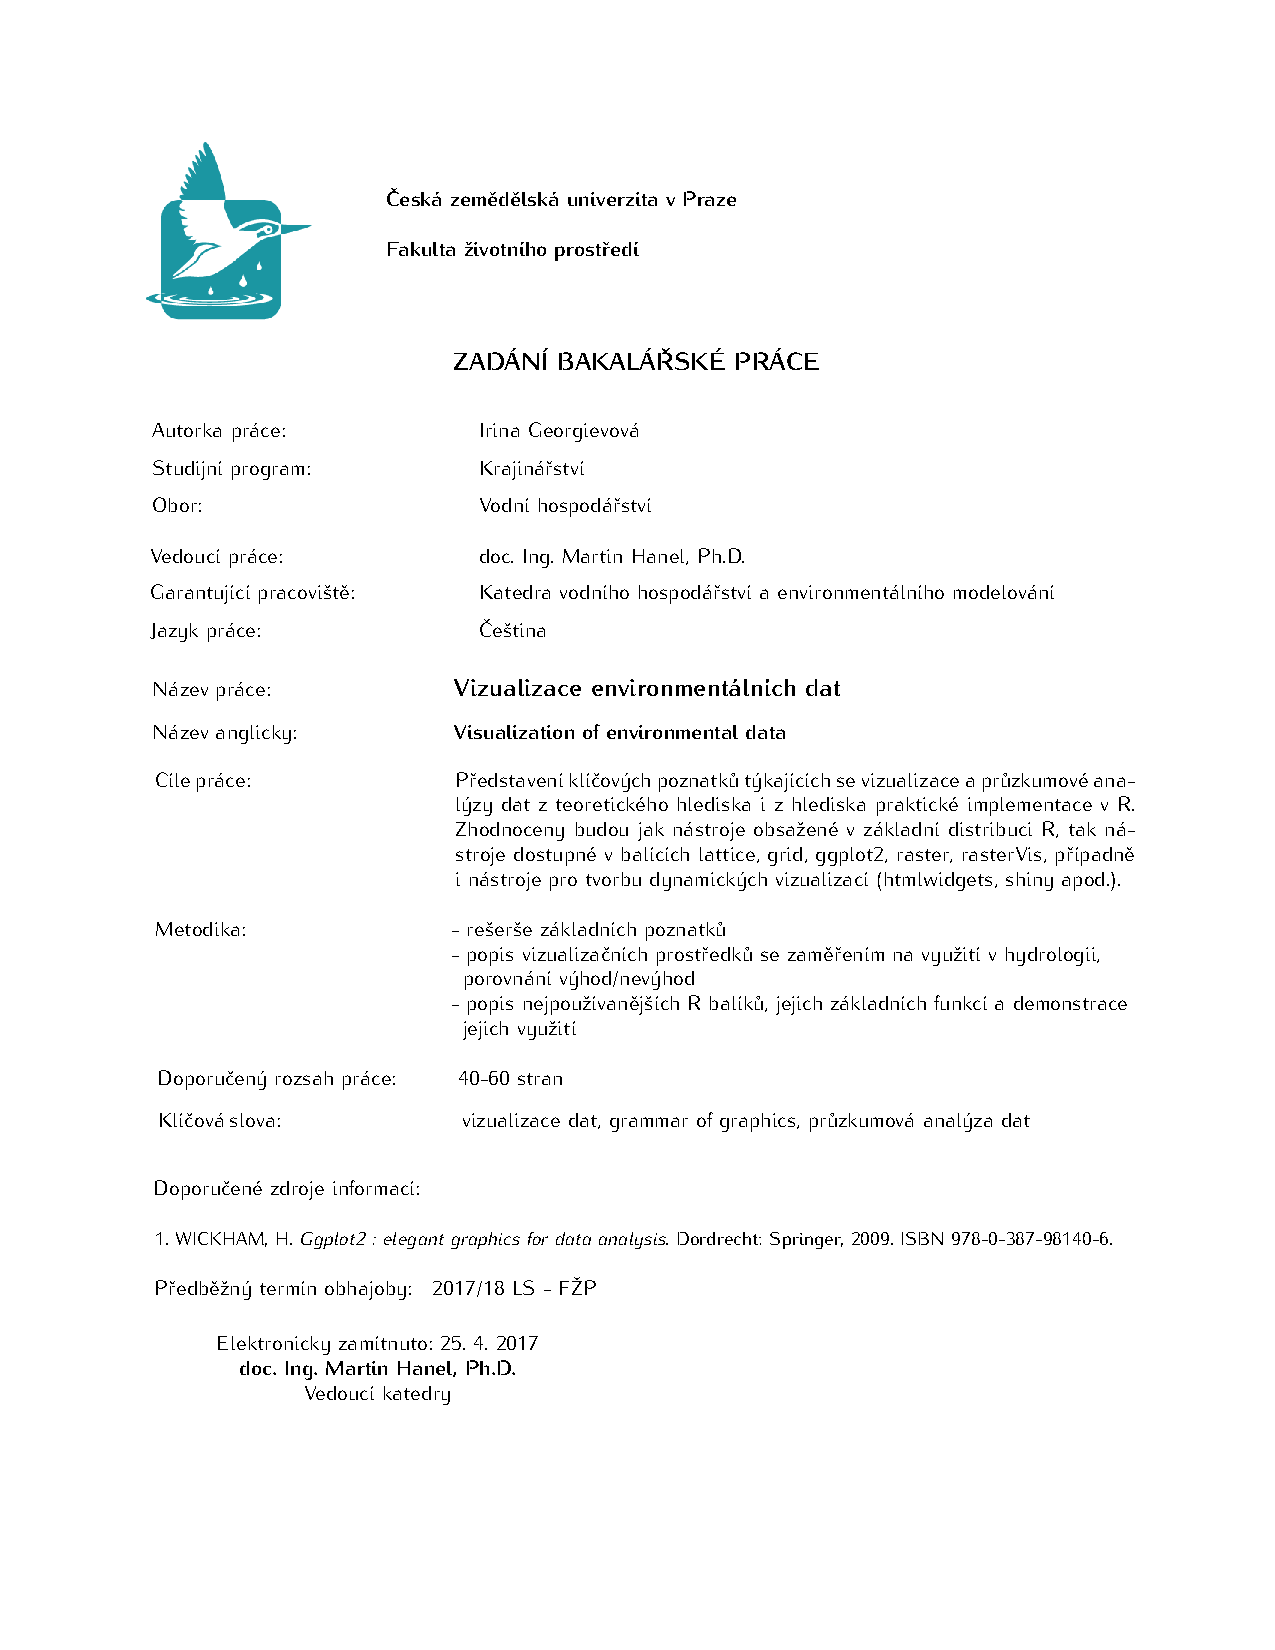
\includepdf[pages={1,2},pagecommand={}, scale = 0.75]{zadani.pdf}
\newpage


\vglue 0pt plus 1fill

\noindent
{\bfseries Prohlášení:} \\
Prohlašuji, že jsem bakalářskou práci \emph{Vizualizace enviromentálních dat} zpracovala samostatně. Veškerou literaturu a další podkladové materiály uvádím v~ seznamu na straně ~\pageref{literatura}.

\vspace{10mm}

\hbox{\hbox to 0.5\hsize{%
V Praze dne ..................
\hss}\hbox to 0.5\hsize{%
\hspace{100pt}...........................
\hss}}

\vspace{1mm}
\hbox{\hbox to 0.5\hsize{%

\hss}\hbox to 0.5\hsize{%
\hspace{100pt}Irina Georgievová
\hss}}

\vspace{20mm}

\newpage

\vglue 0pt plus 1fill
\noindent
{\bfseries Poděkování:} \\

\newpage

\newpage


\vbox to 0.5\vsize{
\setlength\parindent{0mm}
\setlength\parskip{5mm}

{\LARGE\bfseries Abstrakt} 

Práce shrnuje důležité poznatky o vizualizaci dat. Probírá historii jejího vývoje vizualizace a položení vědeckých základů Williamem S. Clevelandem, Edwardem Tuftem a Lelandem Wilkinsonem.  Vizualizace dat je klíčovým nástrojem pro průzkumovou analýzu dat, který je využíván pro jejich lepší pochopení, odhalení neočekávaného chování dat či při rozhodnutí o dalším směru analýzy. Práce dále popisuje nástroje současné  vizualizace dat v programovacím jazyku R a probírá jak základní možnosti softwaru, tak i pokročilé balíčky (\texttt{grid}, \texttt{lattice}, \texttt{ggplot2}, \texttt{raster} a další). Hlavním přínosem práce je tvorba webové aplikace pomocí nástrojů pro dynamickou vizualizací (\texttt{htmlwidgets}, \texttt{Shiny} a \texttt{flexdashboard}).  Aplikace se soustředí na analýzu hydrologické bilance a předpověď sucha v útvarech povrchových vod České republiky a demonstruje veškeré výhody moderní vizualizace dat. 

{\bfseries Klíčová slova: } vizualizace dat, grammar of graphics, průzkumová analýza dat, R, Shiny
\vss}\nobreak\vbox to 0.49\vsize{
\setlength\parindent{0mm}
\setlength\parskip{5mm}
{\LARGE\bfseries Abstract} 



{\bfseries Keywords:  } Data visualization, grammar of graphics, exploratory data analysis, R, Shiny
\vss}

\end{document}


\tableofcontents

\newpage

\listoffigures
\listoftables

\newpage

\section{Úvod}\label{uvod}

\pagestyle{plain} \setcounter{page}{1}

\qquad Vizualizace dat vždy hrála významnou roli v datové analýze. Je to
jeden z~nejlepších, nejjednodušších způsobů pro pochopení a prezentaci
dat. Vizualizace poskytuje jasnou představu o složení dat, odhaluje
skryté struktury v datech a~shrnuje informace. Proces vizualizace je
nedílnou součásti mnoha analýz a téměř všechna odvětví využívají
grafického zobrazení dat k sumarizaci a komunikaci svých výsledků.

\qquad Data z těchto odvětví, která jsou sbírána a analyzována po dobu
mnoha let se čím dat častěji převádějí do grafické formy. Masivní příliv
dat a jejich dostupnost vedly k novým metodám a novým přístupům.
Kombinace programovacích dovedností, matematických a statistických
znalostí a jiných odborných znalostí týkajících se obsahu přijala název
\enquote{\emph{Data Science}} (Rahlf 2017).

\qquad Hlavní výhodou vizualizace je její relativní jednoduchost na
zpracování a dostupnost různých nástrojů k její tvorbě. Avšak nesprávné
či nevhodné použití těchto nástrojů vede k tvorbě grafů, které lze
považovat za nepřehledné, postrádající smysl až zavádějící. Z tohoto
důvodů je vhodné respektovat obecné zásady vizualizace dat a informací.

\qquad Táto bakalářská práce se zabývá shrnutím klíčových poznatků o
vizualizaci a~průzkumové analýze dat, a to jak z teoretického hlediska,
tak i z hlediska praktické implementace v programovacím jazyku R. Jsou
popsány zásady vizualizace, její zařazení do datové analýzy, moderní
způsoby vizualizace a pokročilé R baličky. Součásti práce je také webová
aplikace pro vizualizaci a analýzu hydrologické bilance a předpověď
sucha v útvarech povrchových vod ČR.

\newpage

\section{Cíle práce}\label{cile-prace}

\qquad Práce má dva hlavní cíle. Prvním cílem se zabývá teoretická část,
která shrnuje klíčové poznatky týkajících se zásad vizualizace,
průzkumové analýzy dat a vizualizace v statistickém programovacím jazyku
R. Nejdříve je popsána krátká historie vizualizace, výsledkem které bylo
stanovení jejích zásad. Vývoj vizualizace je těsně propojen s vývojem
statistiky a výpočetní techniky, což se projevilo na vývoji analýzy dat.
Postupně se vizualizace stala jedním z klíčových nástrojů průzkumové
analýzy, která využívá statistické grafy a modelování k lepšímu
pochopení dat. Dále teoretická část obsahuje informace o nástrojích
moderní vizualizace dat v jazyku R, který je v~současnosti jeden z
nejpopulárnějších nástrojů analýzy dat (Developer Survey Results 2017).
Popsány jsou jak základní možností, tak i nejčastěji používané balíčky.
Další cíl této bakalářské práce staví na teoretické částí a využívá
informace v ní obsažené k~vytvoření webové aplikace s interaktivními
prvky pro demonstraci možností moderní vizualizace environmentálních
dat.

\newpage

\section*{Teoretická část}\label{teoreticka-cast}
\addcontentsline{toc}{section}{Teoretická část}

\subsection{1 Vizualizace dat}\label{vizualizace-dat}

\subsubsection{1.1 Historie vizualizace
dat}\label{historie-vizualizace-dat}

\qquad Do 17. století jediné, co by se dalo nazvat jako vizualizace dat
byly mapy pro navigaci a průzkum, ale také diagramy, geometrická
schémata a tabulky pozic hvězd a jiných nebeských těles. Postupný vývoj
statistické teorie a růst zájmu o data na konci 18. století vedly k
inovacím a expanzi nových grafických forem. Kartografové se pokoušeli
zaznamenat více, než pouhou geografickou polohu na mapě a objevily se
první pokusy o tematické mapování geologických, ekonomických a
medicínských dat.

\qquad Wiliam Playfair (1759-1823) je obecně znám jako průkopník v
oblasti vizualizace dat a je považován za vynálezce několika typů grafů.
Například liniový a sloupcový graf či grafy časových řad byly popsány v
jeho atlasu z roku 1786 \textit{"Commercial and Political Atlas"}
(Playfair 1786). Později popsal i koláčový graf ve svém breviáři
\textit{"Statistical Breviary"} z roku 1801 (Playfair 1801). Obrázek
\ref{fig:ch1.0} ukazuje příklad jeho kreativní kombinace různých
vizualizačních technik (kruhy, koláče, linie), pomocí kterých se snažil
porovnat daňovou zátěž mezi Británii a dalšími zeměmi. Na tomto grafu
také ukázal možnost použití více měřítek pro různé ukazatele (graficky
vyjádřena populace a výše daní).

\begin{figure}[H]

{\centering \includegraphics[width=1\linewidth]{fig/Playfair_taxes_population} 

}

\caption{\label{fig:ch1.0} Kombinace různých vizuálních techník, (Playfair 1801)}\label{fig:playfair}
\end{figure}

\newpage

\begin{wrapfigure}[16]{R}{0.45\textwidth}
    \centering
    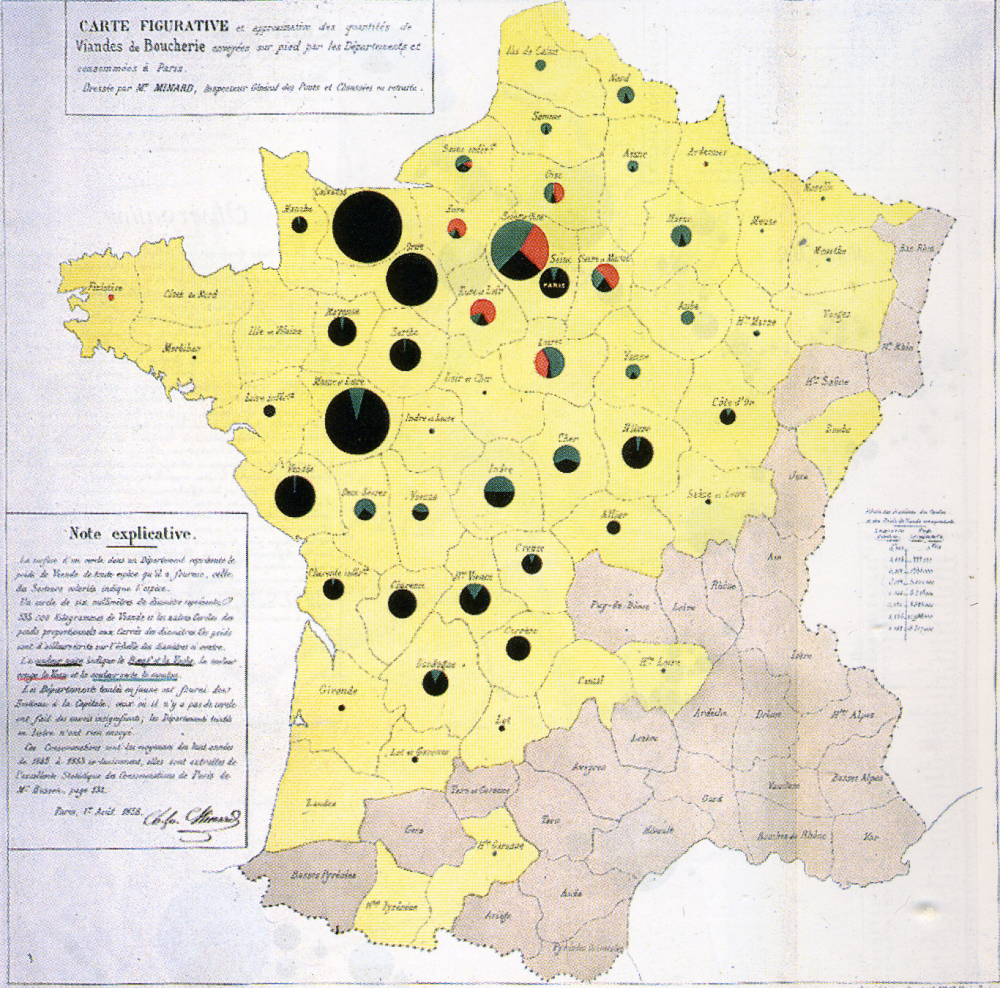
\includegraphics[width=0.42\textwidth]{fig/Minard_1858}
    \vspace{-5pt}
    \caption{Dobytek odeslaný z celé Francie ke spotřebě v Paříži, Minard (1858), převzato z (Palsky 1996)}
    \label{fig:ch1.1}
\end{wrapfigure}

\qquad V polovině 19. století byly vytvořeny všechny podmínky pro rychlý
vývoj vizualizace. V důsledku rostoucí významnosti číselných informací
pro sociální plánovaní, industrializaci, obchod a dopravu byly zřízeny
oficiální statistické úřady po celé Evropě. Rozvoj statistické teorie,
iniciovaný Johannem Carlem Friedrichem Gaussem a Pierrem Simonem de
Laplacem, měl odezvu ve společností a poskytl prostředky ke zpracování
velkého množství dat. Pro vizualizaci dat se stalo období
\mbox{1850-1900} \enquote{zlatým věkem}, s velkým množstvím inovací. S
těmito inovacemi je hlavně spojeno jméno Charlese Josepha Minarda
{[}1781-1870{]}. Minardem bylo například zavedeno použití koláčových
grafů s výsečemi na mapách (obrázek \ref{fig:ch1.1}), kde velikost
koláčového grafu ukazuje sumu sledované proměnné pro každou oblast na
mapě a výseče reprezentují dílčí součty za jednotlivé kategorie. Dále se
také zabýval znázorněním geografických pohybů úměrně jejich velikostí
jako je přeprava lidí, zboží, import či export. Tento typ vizualizace se
nazývá \textit{"flow maps"}, viz obrázek \ref{fig:ch1.2}. Jednou z jeho
nejslavnějších prací je zobrazení postupných ztrát francouzské armády
během Napoleonského tažení na Moskvu v~letech 1812-1813 (obrázek
\ref{fig:ch1.3}), která je považována za nejlepší informativní
vizualizaci vůbec. I~přestože v~tomto grafu je celkem 6 proměnných
(množství, lokace ve dvou rozměrech, postup armády, teplota, datum
a~skupiny), podařilo vše zobrazit tak, aniž by graf byl přeplněný
a~\mbox{matoucí.}

\begin{wrapfigure}[12]{L}{0.51\textwidth}
    \centering
    \vspace*{-20pt}
    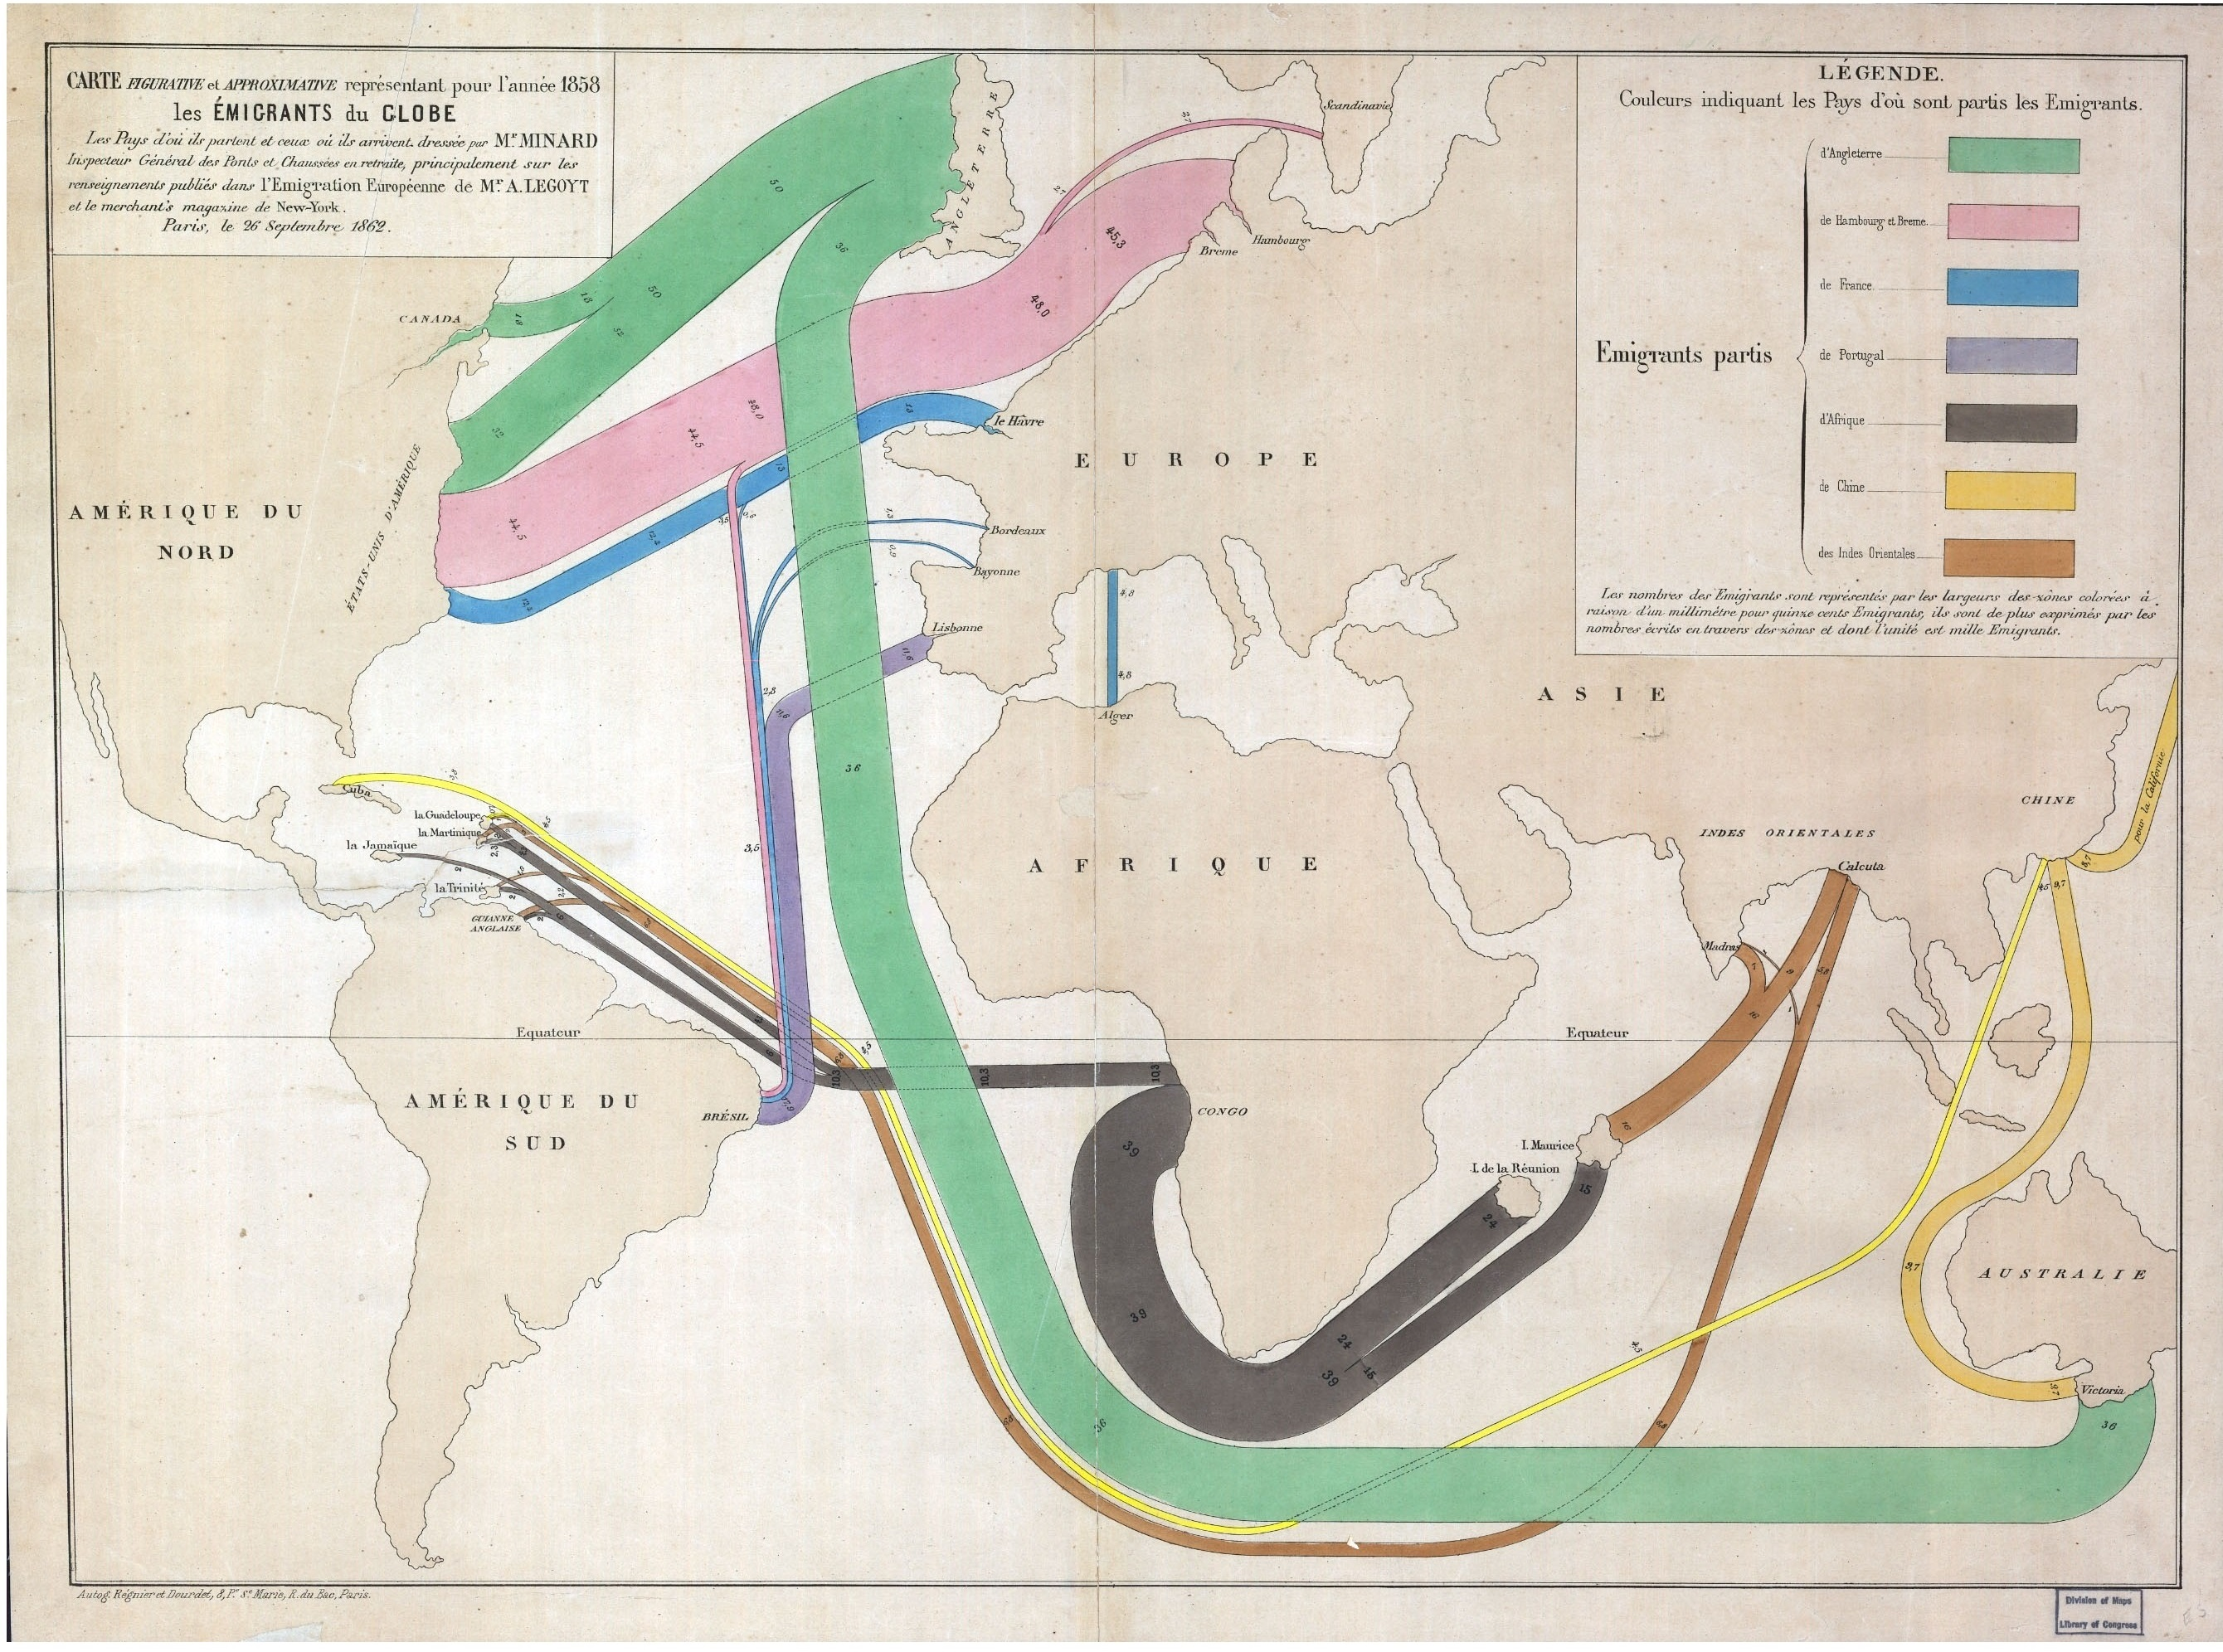
\includegraphics[width=0.5\textwidth]{fig/minard_flow_map.jpg}
    \vspace{-5pt}
    \caption{Mapa světové migrace, (Minard 1858)}
    \label{fig:ch1.2}
\end{wrapfigure}

\vspace{2.5pt} \qquad Začátek 20. století je občas nazýván
\enquote{moderním temným věkem} vizualizace. V letech 1900-1950 bylo jen
málo inovací. Nadšení pro vizualizací, které charakterizovalo 19.
století bylo nahrazeno formálními (z velké části statistickými) grafy a
modely z oblasti sociologie. Hlavní zájem byl o přesná čísla, odhady
parametrů a směrodatné odchylky. Vizualizace byla považována za pouhé
hezké obrázky bez schopnosti podat přesná data. (Friendly 2006)

\begin{figure}[H]
\centering
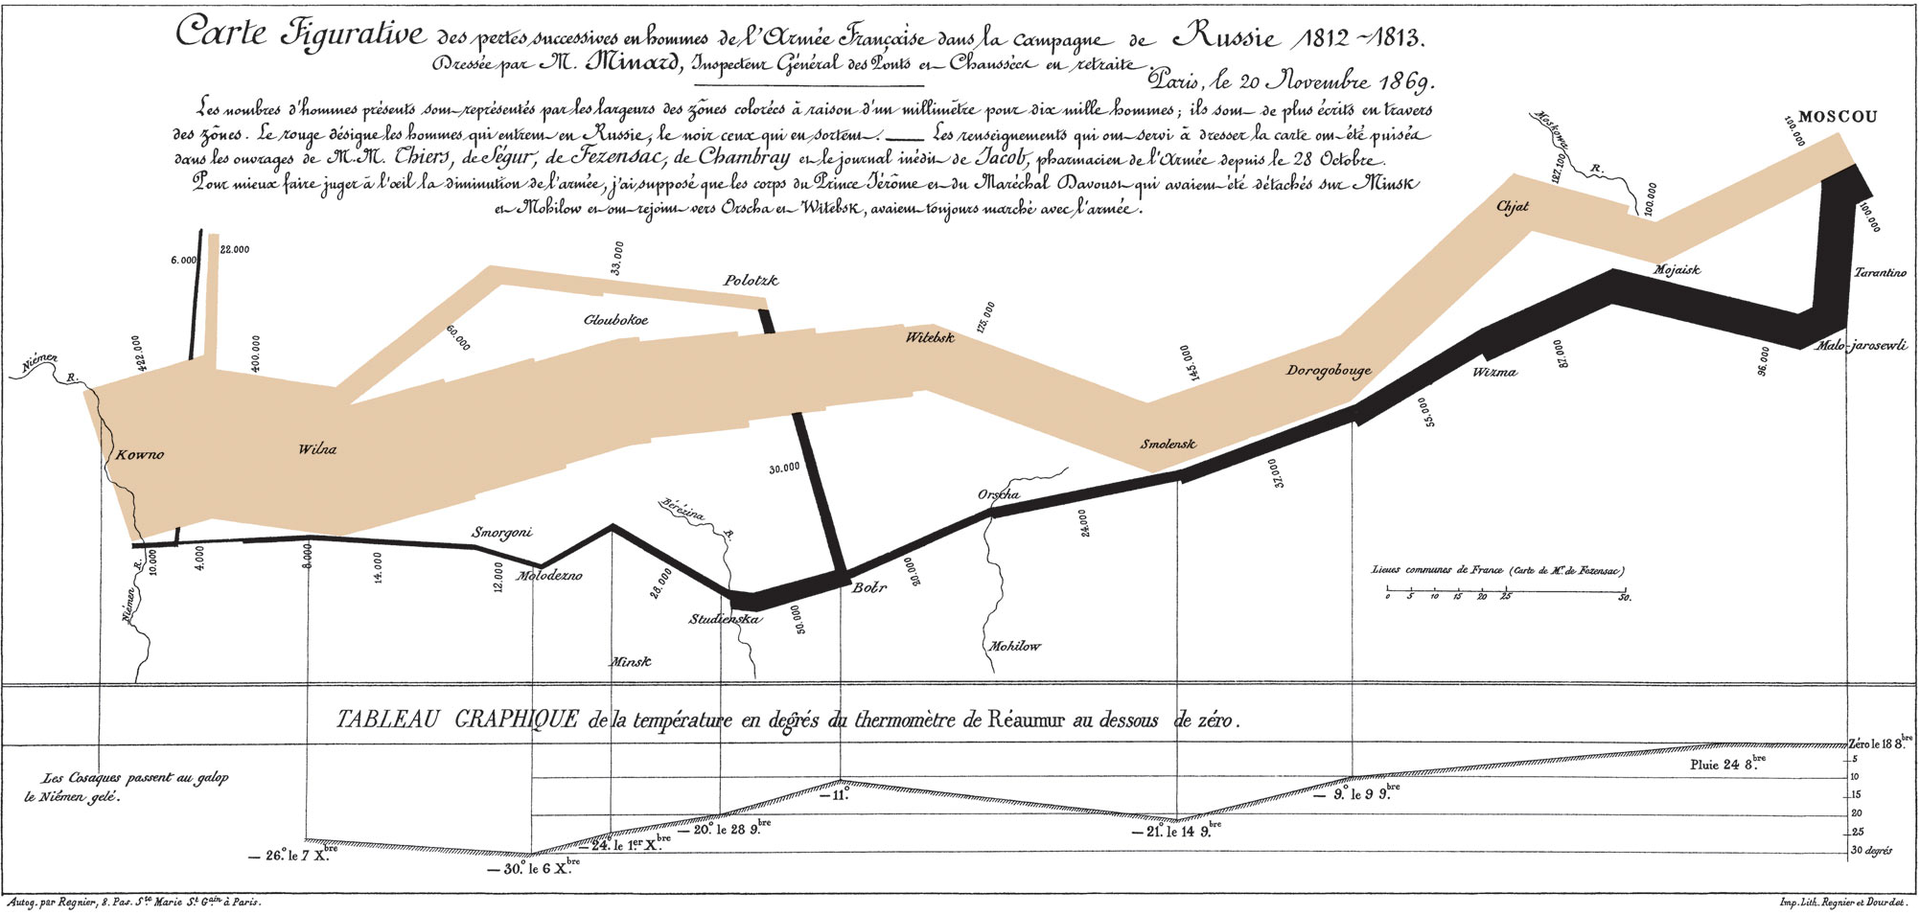
\includegraphics[width = \textwidth]{fig/Minard_1869}
\caption{Postup Napoleonských vojsk v letech 1812-13, Minard (1869)}
\label{fig:ch1.3}
\end{figure}

\qquad Ve své knize \textit{"Graphic Methods for Presenting Facts"} z
roku 1919, Willord C. Brinton {[}1880-1957{]} kritizoval a vysvětloval
chyby takovýchto grafů. Například koláčový graf rozdělení rodinných
příjmů (od 900\$ do 1000\$) na obrázku \ref{fig:ch1.4}. Tento graf je
příkladem nepovedené vizualizace: oko preferenčně soudí dle velikostí
obrázků a ne dle uhlů výsečí. Obrázek uprostřed znázorňuje výdaje za
různé komodity: je to zábavný způsob vizualizace, avšak nelze přesně
určit velikost brašen, ani je porovnat mezi sebou. Další obrázek by měl
čtenáři sdělit informaci, že prodej praček za poslední tří roky vzrostl
sedmkrát. Z obrázku není patrný poměr sedmi ku jedné ani přesné roky kdy
bylo provedeno porovnání údajů. Dále Brinton ve své práci upozorňoval,
že neúspěšná prezentace dat může vést k chybným závěrům a také zmiňoval
potřebu jakéhosi standardu, souhrnu \enquote{gramatických pravidel pro
grafický jazyk} (Brinton 1919).

\begin{figure}[H]

{\centering 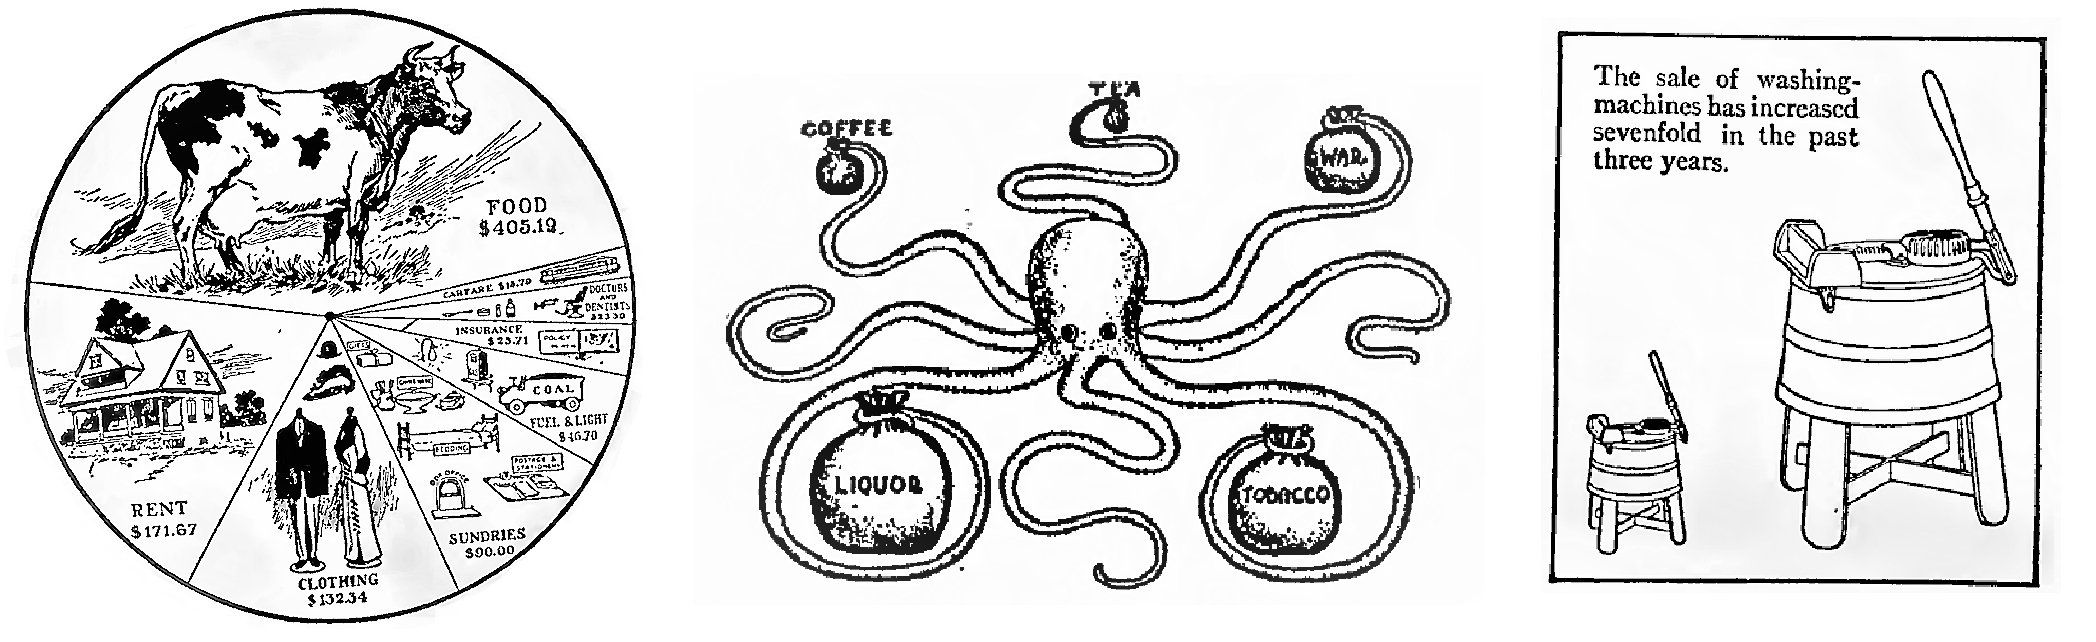
\includegraphics[width=1\linewidth]{fig/brinton} 

}

\caption{\label{fig:ch1.4} Ukázky vizualizací ze začátku 20. století, Brinton 1919}\label{fig:brinton}
\end{figure}

\newpage

\qquad Ke \enquote{znovuzrození} vizualizace došlo v polovině šedesátých
let 20. století po zveřejnění článku Johna W. Tukeyho {[}1915-2000{]}
\textit{"The Future of Data Analysis"}, ve kterém vyzývá společnost k
uznání analýzy dat jako samostatného oboru statistiky odlišného od
statistiky matematické (Tukey 1962). Brzy poté začal Tukey s vývojem
široké řady nových a efektivních grafů pod společným názvem
\enquote{průzkumová analýza dat} (popsáno v jeho knize
\textit{"Explanatory Data Analysis"} z roku 1977, více o tématu viz
kapitola~\protect\hyperlink{EDA}{3})~(Tukey 1977). Mezi těmito novými
grafy je například číslicový histogram (popsaný v~kapitole
\protect\hyperlink{stem-and-leaf}{2.4.3}), boxplot neboli krabicový graf
(popsaný v kapitole \protect\hyperlink{boxplot}{2.3.2}) a~další. Mnoho z
nich je aktivně používáno ve statistické praxi a implementováno do
většiny softwarů~(Friendly 2006).

\subsubsection{1.2 Zásady vizualizace dat}\label{zasady-vizualizace-dat}

\qquad Od roku 1975 se vyvíjí statistické výpočetní systémy a s nimi i
nové metody analýzy a vizualizace dat. V tomto období vizualizace začala
být vnímána jako vlastní odvětví a to především díky Williamu S.
Clevelandovi a Edwardu Tuftemu, kteří položili vědecké základy tohoto
odvětví. Tufte vyvinul a popularizoval terminologii a~základní principy
grafické integrity. Cleveland se zabýval studiemi grafického vnímání,
kognitivních procesů, které lidé používají k pochopení grafů, a rozvíjel
teorii o~správném provedení vizualizace. Výsledek jejich práce se
promítá i do současné doby v podobě kvalitních, interaktivních a
dynamických vizualizací (Friendly 2006).

\hypertarget{tufte}{\paragraph{1.2.1 Edward Tufte}\label{tufte}}

\qquad Za revoluční průlom se považuje kniha Edwarda Tufteho \emph{The
Visual Display of Quantitative Information} z roku 1983, v kombinaci se
dvěma posléze publikovanými knihami \emph{Envisioning Information} a
\emph{Visual Explanations} z roku 1990, resp. 1997, patří mezi
nejznámější publikace na téma vizualizace dat. Právě v těchto
publikacích Tufte originálním způsobem definuje \enquote{standard}
vizualizace (Rahlf 2017). Ideální vizualizace dle Tufteho je stručná,
elegantní a informativní. Příkladem ideálního grafu je pro Tufteho graf
postupu Napoleonských vojsk v letech 1812-13, vytvořený Minardem (viz
obrázek \ref{fig:ch1.3}). Tufte říká, že grafická elegance se často
nachází v jednoduchosti návrhu a komplexnosti dat (Tufte 1990). Tufte
formuluje základní principy vizualizace jako grafickou dokonalost a
grafickou integritu.

\begin{itemize}
\tightlist
\item
  \textbf{Grafická dokonalost} - grafika by měla:

  \begin{itemize}
  \tightlist
  \item
    být o datech a během jejich reprezentace by nemělo dojít ke
    zkreslení
  \item
    vyvolávat otázky o datech, ne o metodologii a technikách vizualizace
  \item
    ukazovat velké množství dat na malém prostoru
  \item
    prezentovat velké datasety souvisle a logicky
  \item
    sloužit rozumnému a jasnému cíli (popisu, průzkumu, \(\dots\))
  \item
    být jednotná se statistickým nebo slovním popisem datasetu
  \end{itemize}
\end{itemize}

\newpage

\begin{itemize}
\tightlist
\item
  Pravidla pro \textbf{grafickou integritu} neboli grafickou celistvost
  a jednoznačnost:

  \begin{itemize}
  \tightlist
  \item
    reprezentace čísel zobrazených v grafu by měla být přímo úměrná
    číselným veličinám datasetu
  \item
    jasná, detailní a svědomitá označení v grafech pro potlačení
    zkreslení, nejasností a dvojznačností
  \item
    popisky jsou důležité
  \item
    v případě časových řad, představujících peníze, používat obecně
    známé jednotky
  \item
    počet rozměrů představených v grafu by neměl přesahovat počet
    proměnných datasetu
  \item
    reprezentace by neměla zahrnovat zavádějící kontext
  \end{itemize}
\end{itemize}

\begin{minipage}[H]{0.475\textwidth}
 \begin{figure}[H]
\centering
    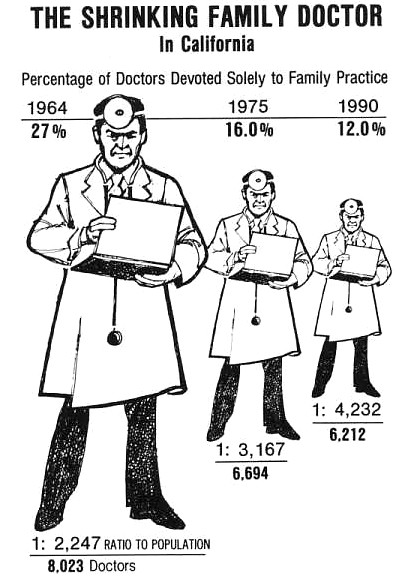
\includegraphics[height = 10.5cm]{fig/tufte_shrinking_doctor}
    \caption{Snižující se procento rodinných lékařů, Los Angeles Times, 1979}
    \label{fig:ch1.5}
 \end{figure}
\end{minipage}\begin{minipage}[H]{0.05\textwidth}
 
\includegraphics[height = 9cm]{fig/blank_v}
\end{minipage}\begin{minipage}[H]{0.475\textwidth}
 \begin{figure}[H]
\centering
    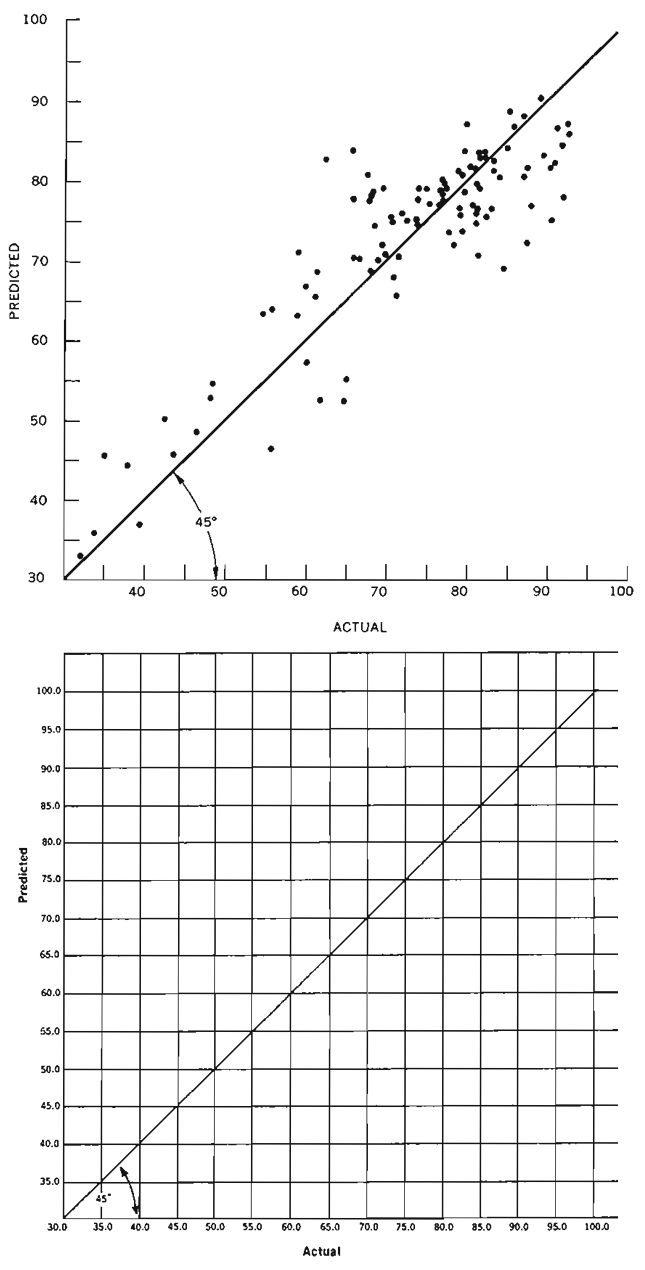
\includegraphics[height = 10.5cm]{fig/data_ink}
    \caption{Vztah skutečné míry volební registrace k předpovídaným hodnotám, převzato E. Tuftem, 1983}
    \label{fig:ch1.6}
 \end{figure}
\end{minipage}

Ve spojení s těmito principy byly zavedeny Edwardem Tuftem následující
termíny:

\begin{itemize}
\item
  \textbf{Lie factor} je definován jako poměr velikosti efektu
  zobrazeného v grafu oproti velikosti efektu v datech. Pokud se rovná
  jedné, považují se reprezentované hodnoty za přesné. Pokud je faktor
  větší než 1.05 či menší než 0.95, indikuje podstatné zkreslení,
  přesahující míru drobných nepřesností vyskytujících se při
  vykreslování grafu. Tufte ve své práci uvádí jako jeden z příkladů
  graf na obrázku \ref{fig:ch1.5}. Tento graf zobrazující snižující se
  procento lékařů věnujících se výhradně rodinné praxi má \emph{lie
  factor} odpovídající hodnotě 2.8, tedy skutečný pokles je značně
  nadhodnocen.
\item
  \textbf{Data ink ratio} - poměr, který vyhodnocuje hustotu grafu a
  obsah informací. Dal by se vyjádřit vzorcem
  \[\textit{Data ink ratio} = \cfrac{\textit{data-ink}}{\textit{celkový inkoust použitý v datech}},\]
  kde \(\textit{data-ink}\) je nezbytné jádro grafu a smazání jakékoliv
  jeho části znamená ztrátu informací. Tento vztah také odpovídá podílu
  grafického inkoustu požitého k vykreslení nepodstatných informací.
  Dalo by se to také vyjádřit jako jedna mínus
  \textit{podíl grafiky, která může být vymazána bez ztráty informací}.
  Tufte doporučuje tento faktor maximalizovat v rozumných mezích,
  nejlépe se vyhnout těžkým mřížkovým liniím na pozadí (dokonce i
  horizontálním referenčním liniím). V příkladu na obrázku
  \ref{fig:ch1.6} jsou zobrazeny dvě verze stejného grafu. Horní má
  hodnotu \emph{data ink ratio} kolem 0.7, dolní graf však, protože
  neobsahuje informaci o datech, pouze nápomocné čáry, má \emph{data ink
  ratio} roven nule.
\item
  \textbf{Chartjunk} - se vztahuje ke všem vizuálním elementům, které
  neslouží ke komunikaci informací zobrazených v grafu nebo odvádějí
  pozornost od těchto informací (Tufte 1983).
\end{itemize}

\hypertarget{cleveland}{\paragraph{1.2.2 Wiliam S.
Cleveland}\label{cleveland}}

\qquad Kromě práce Edwarda Tufteho měly velký vliv i publikace Wiliama
S. Clevelanda. Cleveland se svým kolegou Robertem McGillem publikovali v
roce 1984 článek o~grafickém vnímání (Cleveland a McGill 1984).
Prováděli studie zabývající se rozdílem ve vnímání sloupcových grafů
(pozice a obecné měřítko), koláčových grafů (úhel), skládaných
sloupcových grafů (plocha), barevných a stínovaných map (saturace barev
a stínování) a dalších. Ve svých knihách \emph{Visualizing data} z roku
1993 a \emph{The Elements of Graphing Data} z roku 1994 se Cleveland
zabýval principy vizualizace, grafickými metodami a technikami či
vykreslením tří a více proměnných (rozměrů). Některé z~jeho principů se
shodují s principy vymezenými Tuftem, avšak výzkum Clevelanda v~této
oblasti přesahoval práci Tufteho. Zásady a principy dle Clevelanda by se
daly shrnout do čtyř hlavních kategorií: jasná vize, srozumitelnost,
měřítka a obecné postupy (Cleveland 1994).

\begin{itemize}
\tightlist
\item
  \textbf{Jasná vize}

  \begin{itemize}
  \tightlist
  \item
    Data by měla být středem vizualizace, bez vykreslení nadbytečných
    prvků (neboli \emph{chartjunk} dle Tufteho)
  \item
    K zobrazení dat by se měly používat výrazné grafické prvky.
  \item
    Pro každou proměnnou by měla být použita dvojice os, prostor v takto
    vytvořeném obdélníku je určen k vykreslení grafu, značky na osách by
    měly směrovat mimo oblast grafu.
  \item
    Prostor grafu by neměl být přeplněný (legenda mimo oblast grafu
    atd.).
  \item
    Počet značek na osách by měl být přiměřený.
  \item
    Pokud je to vhodné, referenční linie mohou být použity, avšak
    nesmějí zasahovat do dat.
  \item
    Popisky by neměly zasahovat do kvantitativních dat a nesmějí
    znepřehledňovat graf.
  \item
    Značky a klíče by se měly vyskytovat mimo oblast grafu (případně
    v~legendě), totéž se týká poznámek a nadpisů, které mohou být také
    umístěny do textu.
  \item
    Překrývající se datasety či symboly musí být vizuálně snadně
    rozpoznatelné.
  \item
    Jasnost obrazu musí být zachována při reprodukci i při snížení
    kvality a~zmenšení rozlišení.
  \end{itemize}
\end{itemize}

Cleveland jako příklad špatně zpracované vizualizace vybral graf
\ref{fig:ch1.7a}, na kterém je zobrazeno množství izotopu xenonu
\({}^{133}\mbox{Xe}\) ve vzduchu (\(pCi.m^{-3}\)) po havárii elektrárny
Three Mile Island v Albany, ve státě New York koncem března a začátkem
dubna roku 1979. Vše, včetně popisků os, klíčů a popisků dat bylo
umístěno do oblasti grafu, není dodržena žádná ze zásad Clevelanda.
Výsledkem je matoucí graf, který je obtížně čitelný. Stejná data byla
vizualizována Clevelandem na grafu \ref{fig:ch1.7b} s dodržením
veškerých zásad: odstranění zbytečných objektů a detailů z oblasti
grafu, datasety se zobrazují ve vlastních panelech, oprava popisků
popisujících měření.

\begin{figure}[H]
  \begin{subfigure}{0.57\textwidth}
  \centering
    \vspace*{0.65cm}
      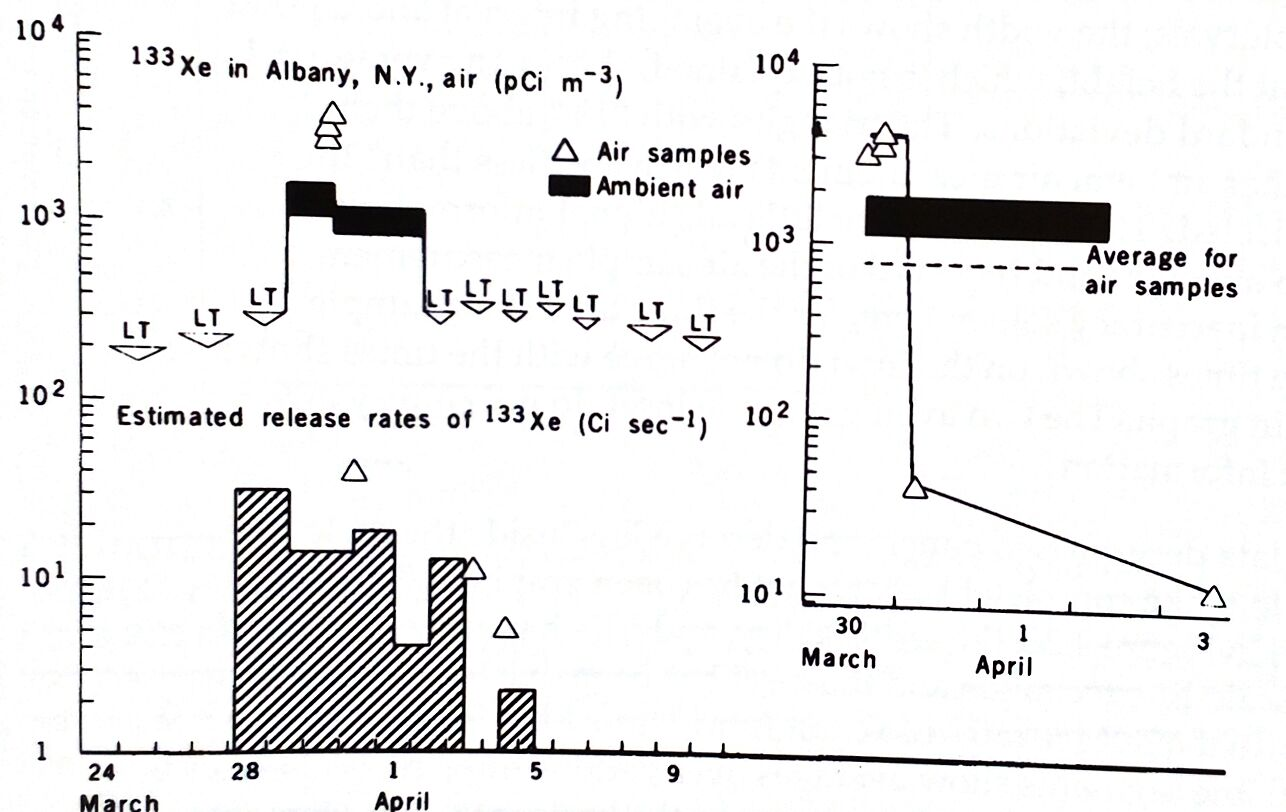
\includegraphics[width=\textwidth]{fig/cleveland_xenon_133}
      \vspace*{0.2cm}
      \caption{}
      \label{fig:ch1.7a}
  \end{subfigure}%
  \begin{subfigure}[H]{0.43\textwidth}
  \centering
      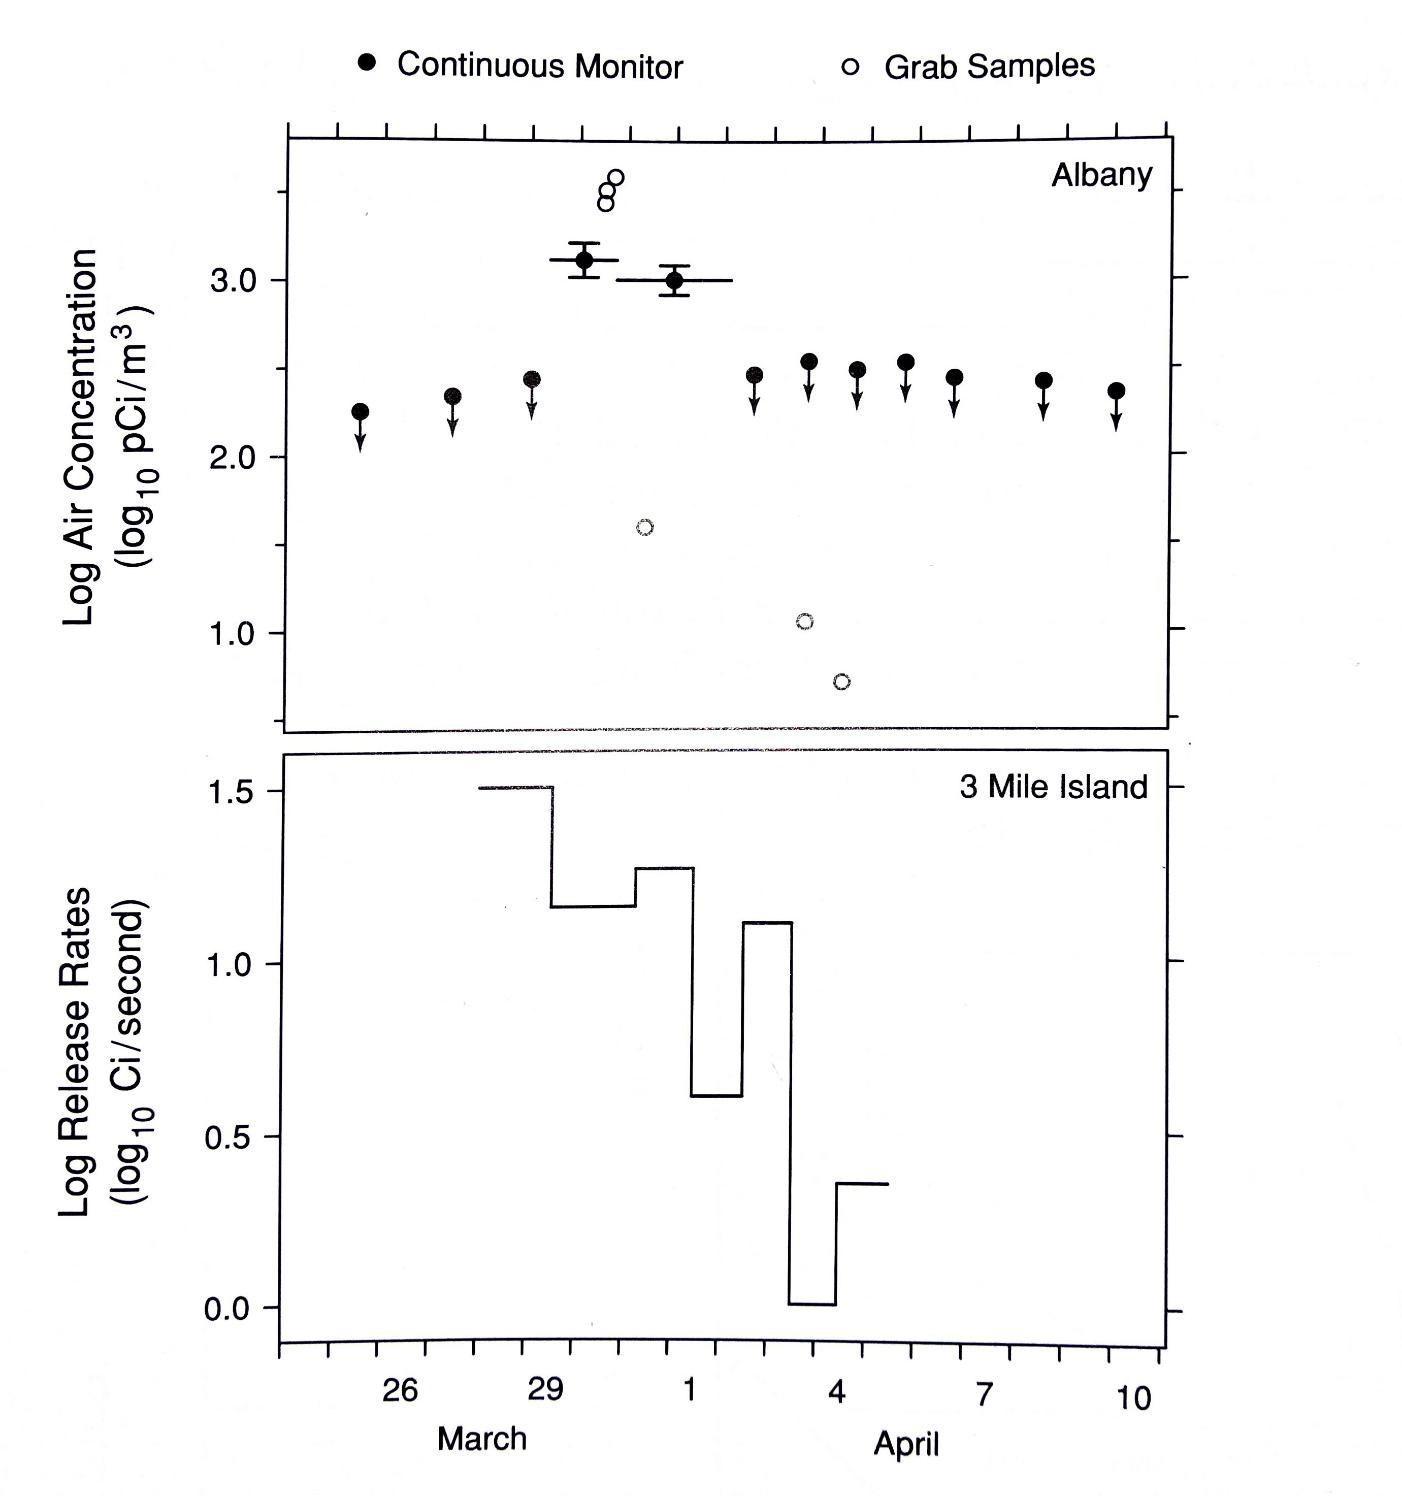
\includegraphics[width=\textwidth]{fig/cleveland_xenon_opr}
      \vspace*{-0.8cm}
      \caption{}
      \label{fig:ch1.7b}
  \end{subfigure}
\vspace*{-0.25cm}
\caption{Radioaktivní oblak při havárii elektrárny Three Mile Island: ${}^{133}\mbox{Xe}$ ve vzduchu ve vzdálenosti \SI{375}{\kilo\meter} (a) a stejný graf přepracovaný Clevelandem (b), 1994} 
\label{fig:ch1.7}
\end{figure}

\begin{itemize}
\tightlist
\item
  \textbf{Jasná srozumitelnost}

  \begin{itemize}
  \tightlist
  \item
    Hlavní závěry by měly být obsaženy v grafické formě. Legenda a
    nadpisy by měly být srozumitelné a vyčerpávající.
  \item
    Grafy by měly být zkontrolovány.
  \item
    Mělo by se usilovat o přehlednost (viz \enquote{jasná víze}).
  \end{itemize}
\end{itemize}

\newpage

\begin{itemize}
\tightlist
\item
  \textbf{Měřítka}

  \begin{itemize}
  \tightlist
  \item
    Volit rozsah os tak, aby obsahoval, případně téměř obsahoval, rozsah
    dat.
  \item
    Volit takové měřítko, aby data vyplňovala co největší prostor.
  \item
    Občas je užitečné mít pro proměnnou dvě osy pro rozdílná měřítka.
  \item
    Volit vhodné měřítko pokud data jsou porovnávány na více panelech.
  \item
    Osy grafu nemusejí vždy nutně zahrnovat nulu pro ukázku rozsahu.
  \item
    Použít logaritmická měřítka, když je důležité pochopit procentní
    změny nebo multiplikativní faktory.
  \item
    Použít přerušené měřítko pouze v případě potřeby. Alternativou může
    být logaritmizace měřítka.
  \end{itemize}
\item
  \textbf{Obecné postupy}

  \begin{itemize}
  \tightlist
  \item
    Velké množství kvantitativní informace může být vměstnáno do
    relativně malých oblastí.
  \item
    Tvorba grafů by měla být opakující se, iterativní a experimentální
    činností.
  \item
    Data by měla být vykreslena tolikrát, kolikrát je třeba.
  \item
    Užitečné grafy vyžadují pečlivou a detailní práci.
  \end{itemize}
\end{itemize}

\qquad Cleveland se mimo jiné podílel na tvorbě řady technik pro
prohlížení komplexních datových sad s více proměnnými, kterým se říká
\textit{Trellis Graphics} nebo \textit{Trellis Plots}. Technika obdržela
svůj název \textit{trellis} kvůli obvyklému výsledku řady obdélníkových
grafů, připomínajících zahradní mříž. Na obrázku \ref{fig:ch1.8} je
ukázka \emph{trellis} grafu, zobrazující údaje o emisích motoru (Becker
et al. 1996).

\begin{figure}[H]
\centering
    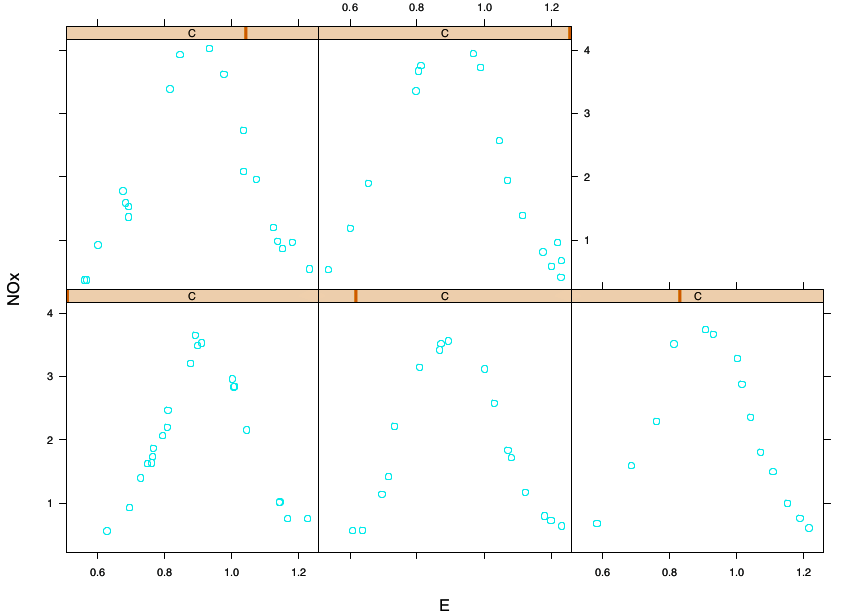
\includegraphics[height = 0.4\textheight]{fig/trellis}
    \caption{\textit{Trellis} graf, zobrazující údaje o emisích motoru, Becker et al., 1996}
    \label{fig:ch1.8}
 \end{figure}

\newpage

\hypertarget{gg}{\subsubsection{1.3 Grammar of graphics}\label{gg}}

\vspace*{-0.35cm} \qquad \textit{The Grammar of Graphics} publikována
Lelandem Wilkinsonem v roce 2005 (Wilkinson 2005) detailně popisuje
prvky, které tvoří základ všech statistických grafů a odpovídá na
základní otázku: co je statistická grafika? (Wickham 2010b) Tato
publikace měla extrémně velký vliv na myšlení o grafech. Hadley Wickham
na základě Wilkinsonovy gramatiky publikoval v roce 2009 článek \emph{A
Layered Grammar of Graphics} (Wickham 2010a), který se zaměřuje primárně
na vrstvy vizualizační grafiky a jejich zapojení do jazyka R. Následně
také pro něj posloužila jako inspirace pro tvorbu balíčku
\texttt{ggplot} (viz kapitola \protect\hyperlink{ggplot}{4.1.3}).

\qquad \textit{The Grammar of Graphics} říká, že statistická grafika je
mapováním dat k~estetickým atributům (barva, tvar, velikost)
geometrických objektů (body, linie, sloupce). Graf také může obsahovat
statistickou transformaci dat a být vykreslen ve specifickém
souřadnicovém systému. \emph{Faceting} může být použit k vygenerování
stejného grafu pro různé podmnožiny datasetu. Kombinace těchto
nezávislých komponent tvoří grafiku. Jednotlivé komponenty tvořící graf,
dle Wilkinsonovy syntaxe, lze zapsat následovně:

\begin{itemize}
\tightlist
\item
  Vizualizovaná \textbf{data} a soubor estetických mapování
  (\textbf{mapping}s) popisujících jak jsou proměnné z dat mapovány na
  vnímané estetické atributy.
\item
  Geometrické objekty (\textbf{geom}s) reprezentují to, co je doopravdy
  na grafu: body, linie, polygony atd.
\item
  Statistické transformace (\textbf{stat}s) sumarizují data mnoha
  užitečnými způsoby. Jako příklad by se daly použít výpočty intervalů a
  počty pozorování při tvorbě histogramu (kapitola
  \protect\hyperlink{hist}{2.4.1}) nebo tvorba lineárního modelu.
  Statistické transformace patří k nepovinným, ale velmi užitečným
  komponentům.
\item
  Měřítka (\textbf{scale}s) reprezentují hodnoty v datovém prostoru
  převedené na hodnoty v estetickém prostoru, ať už se jedná o barvu,
  velikost či tvar. Na měřítku závisí legenda a osy, tvořené inverzním
  mapováním umožňující číst z grafu původní hodnoty datasetu.
\item
  Souřadnicový systém (\textbf{coord}) popisuje, jak jsou souřadnice dat
  mapovány do roviny grafiky. Rovněž poskytuje osy a mřížky, umožňující
  čtení grafů. Běžně se používá kartézský souřadnicový systém, ale je k
  dispozici i řada dalších systémů včetně polárních souřadnic a mapových
  projekcí.
\item
  Specifikace \textbf{facet}ingu popisuje, jaké proměnné by měli být
  použity k rozdělení dat na podmnožiny a jak by tyto podmnožiny měly
  být uspořádány. Jedná se o mocný nástroj pro zkoumání toho, zda jsou
  statistické modely stejné nebo odlišné v různých podmínkách.
\end{itemize}

\qquad Je také důležité zmínit, o čem Wilkinsova gramatika není.
Nenaznačuje jaký typ grafů by se měl použít k zodpovězení otázek o
datech, jak to dělali Cleveland (Cleveland 1993) nebo Tukey (Tukey
1977), zaměřuje se konkrétně na jejich tvorbu. Ironií je, že
\textit{The Grammar of Graphics} neurčuje, jak by měla vypadat grafika,
nespecifikuje velikost písma ani barvu pozadí (Wickham 2010b). Otázkou
vzhledu grafů se zabývali Tufte a Cleveland (kapitoly
\protect\hyperlink{tufte}{1.2.1} a
\protect\hyperlink{cleveland}{1.2.2}). Dále Wilkinsova gramatika
nepopisuje interaktivní ani dynamické vizualizace, obsahuje pouze
statické grafy. Při tvorbě dynamických či interaktivních grafů je třeba
se obrátit na jiný zdroj, například \emph{Interactive Data Visualization
for the Web} od Scottea Murrayho (Murray 2013) nebo \emph{Interactive
Visualization} od Billa Ferstera~(Ferster 2012).

\hypertarget{base}{\subsection{2 Základní grafy v R}\label{base}}

\qquad Pro vytváření základních grafů v R používáme vestavěný balíček
\texttt{graphics}, který obsahuje mnoho užitečných funkcí pro tvorbu
grafických prvků (R-Documentation {[}vid. 22.4.2017{]}). Tato kapitola
se soustředí na tento balíček, zatímco v kapitole
\protect\hyperlink{pokrocila}{4} jsou popsány funkce dalších široce
používaných balíčků (například \texttt{lattice}
\protect\hyperlink{lattice}{4.1.2} či \texttt{ggplot2}
\protect\hyperlink{ggplot}{4.1.3}), které nabízí podobné funkce, avšak s
různým rozsahem nastavení (Teetor 2011).

\qquad V následujících příkladech nejsou grafy doplněny o barvy, popisky
os, legendy ani názvy a to především proto, že záměrem této kapitoly je
popsat základní grafy a funkce pro jejich tvorbu v prostředí R. Všechny
tyto prvky mohou být přidány do grafu, ale tím by příklady obsahovali
irelevantní parametry vzhledem k zaměření této kapitoly. Základní funkce
\texttt{plot(x)} jejímž voláním se obdrží pole s grafickou reprezentaci
proměnné \enquote{x}, by při doplnění kódu o veškeré parametry vypadala
následovaně (Teetor 2011):

\begin{Shaded}
\begin{Highlighting}[]
\KeywordTok{plot}\NormalTok{(x, }\DataTypeTok{main =} \StringTok{"Název grafu"}\NormalTok{, }\DataTypeTok{xlab =} \StringTok{"popis osy x"}\NormalTok{, }
\OperatorTok{+}\StringTok{    }\DataTypeTok{ylab =} \StringTok{"popis osy y"}\NormalTok{, }\DataTypeTok{col =} \KeywordTok{c}\NormalTok{(}\StringTok{"red"}\NormalTok{, }\StringTok{"black"}\NormalTok{, }\StringTok{"green"}\NormalTok{)) }
\end{Highlighting}
\end{Shaded}

Záměrem je tedy používání příkazů s pouze relevantními parametry.

\hypertarget{scatterplot}{\subsubsection{2.1 Bodový
graf}\label{scatterplot}}

\qquad Bodový graf je rychlým způsobem, jak znázornit vztahy a
souvislosti mezi proměnnými datasetu, případně k zjištění jejich
neexistence. Data jsou zobrazena v~kartézském souřadném systému a mají
pro každou hodnotu proměnné dané místo na vodorovné a svislé ose. V
případě existence závislostí mezi proměnnými lze tuto závislost
interpolovat přímkou, křivkou či dalším vhodným vyobrazením této
závislosti.

\qquad Pro vytvoření bodového grafu v základním prostředí R (pomocí
\texttt{graphics}) použijeme funkci \texttt{plot()}, která má tento typ
grafu předdefinovaný jako výchozí pro numerické hodnoty. Viz obrázek
\ref{fig:ch2.1} (a). Nečíselná data vytvoří jiný typ grafu.

\begin{Shaded}
\begin{Highlighting}[]
\KeywordTok{plot}\NormalTok{(cars)}
\end{Highlighting}
\end{Shaded}

\subsubsection{2.2 Liniový graf}\label{liniovy-graf}

\qquad Jediný rozdíl mezi bodovým a liniovým grafem je, že jeden
zobrazuje body a~druhý je spojuje (Teetor 2011) (viz obrázek
\ref{fig:ch2.1} (a), (b)). Pro vykreslení liniového grafu se používá již
několikrát zmíněná funkce \texttt{plot()}, kterou doplníme o požadovaný
typ vykreslení:

\begin{Shaded}
\begin{Highlighting}[]
\KeywordTok{plot}\NormalTok{(x, }\DataTypeTok{type=}\StringTok{"l"}\NormalTok{)}
\end{Highlighting}
\end{Shaded}

V tabulce \ref{tab1} jsou uvedené některé základní atributy parametru
\texttt{type}, které mohou být použity (R-Documentation {[}vid.
11.5.2017{]}):

\begin{table}[H]
\centering
\begin{tabular}{|c|c|c|}
\hline
  & anglický popis & český popis    \\ \hline
p & points         & bodový         \\ \hline
l & lines          & liniový        \\ \hline
b & both           & složený        \\ \hline
h & histogram      & tyčkový        \\ \hline
n & no plotting    & bez vykreslení \\ \hline
\end{tabular}
\caption{Základní atributy parametru `type`}
\label{tab1}
\end{table}

\begin{figure}[H]

{\centering 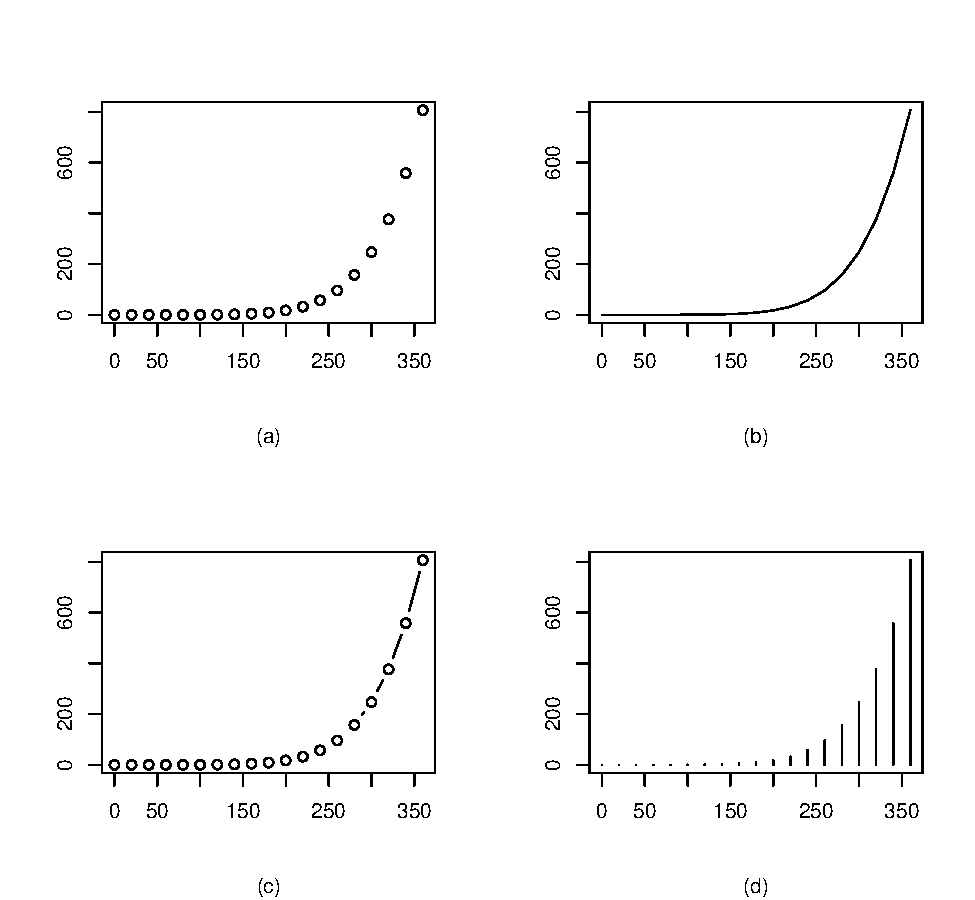
\includegraphics[width=0.8\linewidth]{BP_files/figure-latex/graf_typy-1} 

}

\caption{\label{fig:ch2.1} Porovnání základních typů grafů: (a) - bodový, (b) - liniový, (c) - složený, (d) - histogram}\label{fig:graf_typy}
\end{figure}

Popis a všechny atributy dalších parametrů funkce \texttt{plot()} lze
nalézt v nápovědě zadáním příkazu \texttt{?plot()}.

\hypertarget{distribution}{\subsubsection{2.3 Vykreslení rozdělení v
R}\label{distribution}}

\qquad Teorie pravděpodobnosti je základem statistiky a R má hodně
nástrojů pro práci s pravděpodobností, rozdělením pravděpodobnosti a
náhodnými proměnnými. R má zkrácený název pro každé rozdělení
pravděpodobnosti (Teetor 2011). Tyto názvy slouží k~identifikaci funkcí
spojených s rozděleními. Například zkrácený název \enquote{norm} pro
normální rozdělení, \enquote{exp} pro exponenciální rozdělení a další.
Funkce pak mají formu:

\begin{table}[H]
\centering
\begin{tabular}{|l|l|}
\hline
funkce & \multicolumn{1}{c|}{účel}                    \\ \hline
dxxxx  & hustota pravděpodobnosti                     \\ \hline
pxxxx  & distribuční funkce                           \\ \hline
qxxxx  & kvantilová funkce                            \\ \hline
rxxxx  & generátor náhodných čísel z daného rozdělení \\ \hline
\end{tabular}
\caption{Funkce pro práci s rozděleními}
\label{tab2}
\end{table}

Funkce v R lze vykreslovat pomocí funkce \texttt{curve()} z balíčku
\texttt{graphics}. Lze vykreslit jak standardní funkce, tak i funkce
definované uživatelem. Například hustotu pravděpodobnosti normálního
rozdělení a její distribuční funkci můžeme vykreslit tímto způsobem
(Obrázek \ref{fig:ch2.2}):

\begin{Shaded}
\begin{Highlighting}[]
\KeywordTok{curve}\NormalTok{(}\KeywordTok{dnorm}\NormalTok{(x))}
\KeywordTok{curve}\NormalTok{(}\KeywordTok{pnorm}\NormalTok{(x))}
\end{Highlighting}
\end{Shaded}

\begin{figure}[H]

{\centering 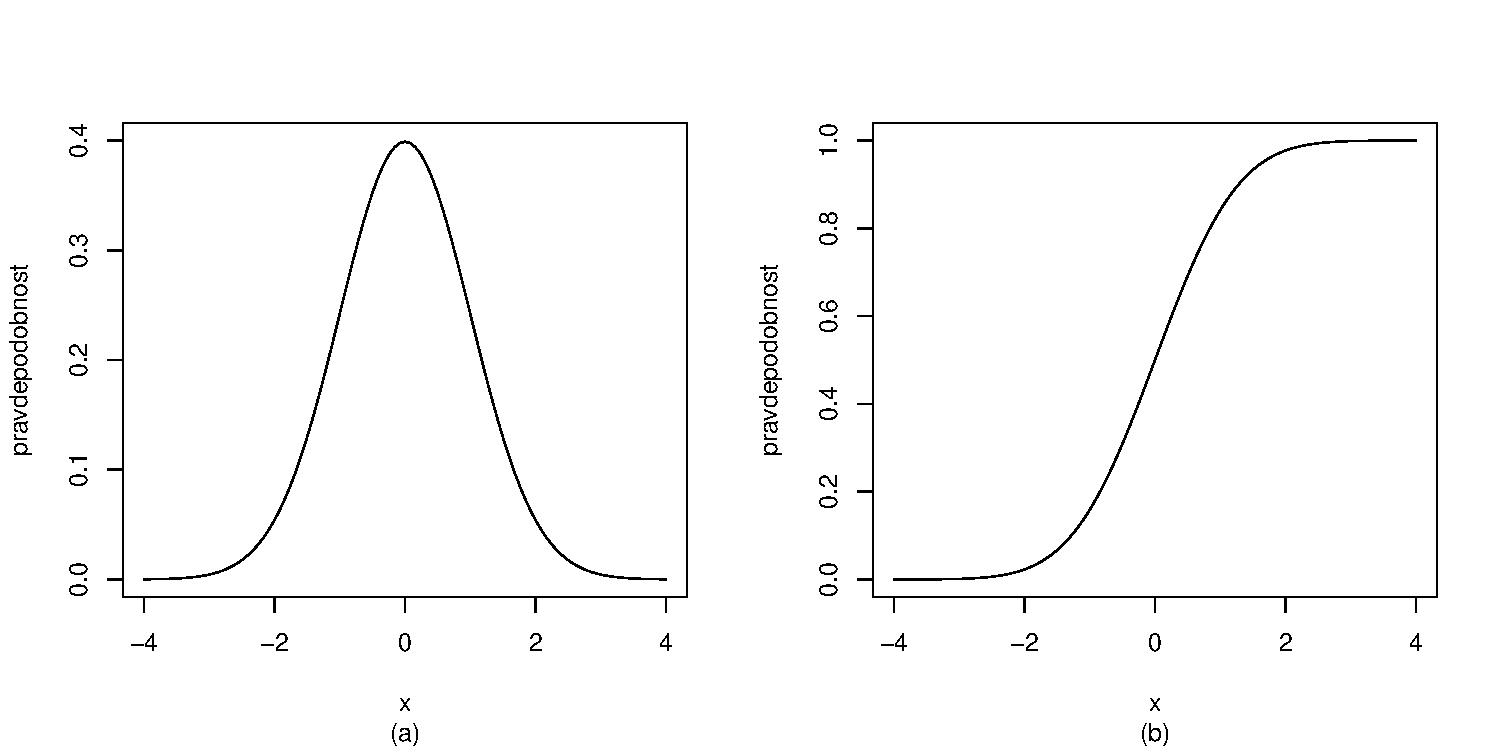
\includegraphics{BP_files/figure-latex/normal-1} 

}

\caption{\label{fig:ch2.2} Hustota pravděpodobnosti normálního rozdělení (a) a její distribuční funkce (b)}\label{fig:normal}
\end{figure}

\newpage

\hypertarget{qqpp}{\paragraph{2.3.1 Q-Q graf a P-P graf}\label{qqpp}}

\qquad Q-Q (\emph{quantile-quantile}) graf a P-P
(\emph{probability--probability} nebo \emph{percent--percent}) graf
(Obrázek \ref{fig:ch2.3}) se používají hlavně k testování normality při
průzkumové analýze dat \protect\hyperlink{normtests}{3.4}. Další způsob,
jak zjistit zda-li data mají normální rozdělení je sestrojení histogramu
(viz. sekce \protect\hyperlink{hist}{2.4.1}), avšak použití Q-Q grafu je
přesnější.

\qquad Princip Q-Q grafu spočívá v porovnání dvou rozdělení
pravděpodobnosti pomocí vykreslení jejich kvantilů proti sobě. Na jedné
ose se nacházejí teoretické kvantily normálního rozdělení (nebo jiného
vybraného rozdělení) a na druhé ose kvantily naměřené (pozorované).
Pokud data mají přesně požadované rozdělení, všechny body grafu leží na
přímce pod úhlem 45°. Vztah hustoty rozdělení a Q-Q grafu je znázorněn
na obrázku \ref{fig:ch3.4}. (Teetor 2011) (Cleveland 1994)

\qquad Princip P-P grafu je obdobný jako u Q-Q grafu: vykreslují se dvě
distribuční funkce proti sobě (jedná teoretická a jedná pozorovaná) a
pokud všechny body grafu leží přibližně na přímce, jedná se
pravděpodobně o požadované rozdělení. \mbox{P-P}~graf se často používá k
vyhodnocení koeficientu šikmosti rozdělení (Gibbons a Chakraborti 2003).

V R se Q-Q graf vykreslí takto:

\begin{Shaded}
\begin{Highlighting}[]
\KeywordTok{qqnorm}\NormalTok{(x)}
\KeywordTok{qqline}\NormalTok{(x)}
\end{Highlighting}
\end{Shaded}

P-P graf v R lze vykreslit například následovně:

\begin{Shaded}
\begin{Highlighting}[]
\KeywordTok{plot}\NormalTok{(}\KeywordTok{ppoints}\NormalTok{(}\KeywordTok{length}\NormalTok{(x)), }\KeywordTok{sort}\NormalTok{(}\KeywordTok{pnorm}\NormalTok{(x)))}
\KeywordTok{abline}\NormalTok{(}\DecValTok{0}\NormalTok{,}\DecValTok{1}\NormalTok{)}
\end{Highlighting}
\end{Shaded}

\begin{figure}[H]

{\centering 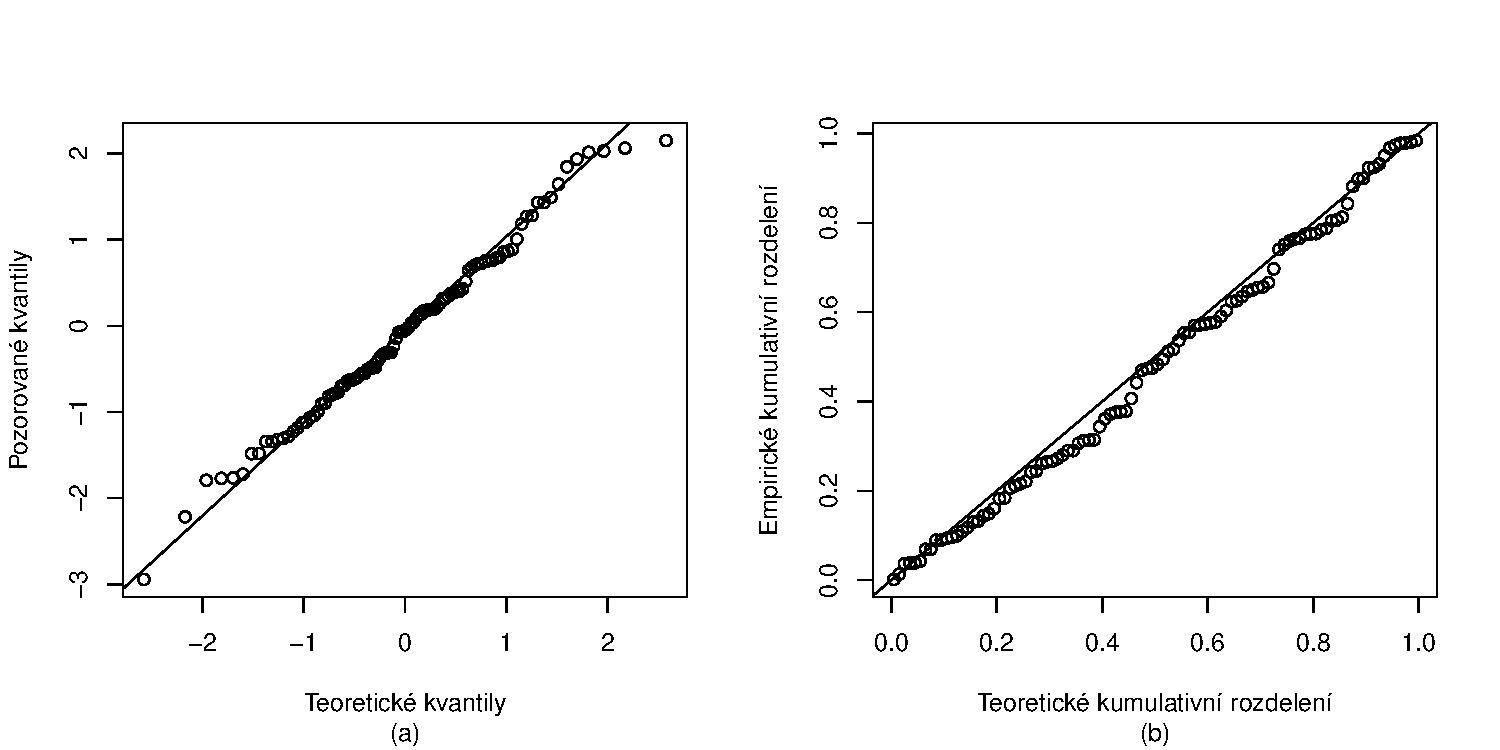
\includegraphics{BP_files/figure-latex/pp-qq plots-1} 

}

\caption{\label{fig:ch2.3} Q-Q Graf (a) a P-P Graf (b)}\label{fig:pp-qq plots}
\end{figure}

\newpage

\hypertarget{boxplot}{\paragraph{2.3.2 Krabicový graf}\label{boxplot}}

\qquad Krabicový graf poskytuje rychlé a jednoduché vizuální shrnutí
datasetu. V~základním prostředí R se vykreslí pomocí funkce
\texttt{boxplot()} z balíčku \texttt{graphics}. Obrázek \ref{fig:ch2.4}
znázorňuje typický krabicový graf, kde silná čára je medián, krabice
kolem ní určuje polohu prvního a třetího kvartilu (dolní
Q\textsubscript{1} kvantil 25\% a horní Q\textsubscript{3} kvantil
75\%). ''Vousy`` (\emph{whiskers}) nad a pod krabicí znázorňují rozpětí
dat bez odlehlých hodnot. Odlehlé hodnoty jsou definovaný jako hodnoty
ležící ve větší vzdálenosti od krabice než 1,5 \(\times\) IQR, kde IQR
je mezikvartilové rozpětí (\emph{interquartile range}) neboli
\(Q_3 - Q_1\).

\begin{Shaded}
\begin{Highlighting}[]
\KeywordTok{boxplot}\NormalTok{(x)}
\end{Highlighting}
\end{Shaded}

\begin{figure}[H]

{\centering 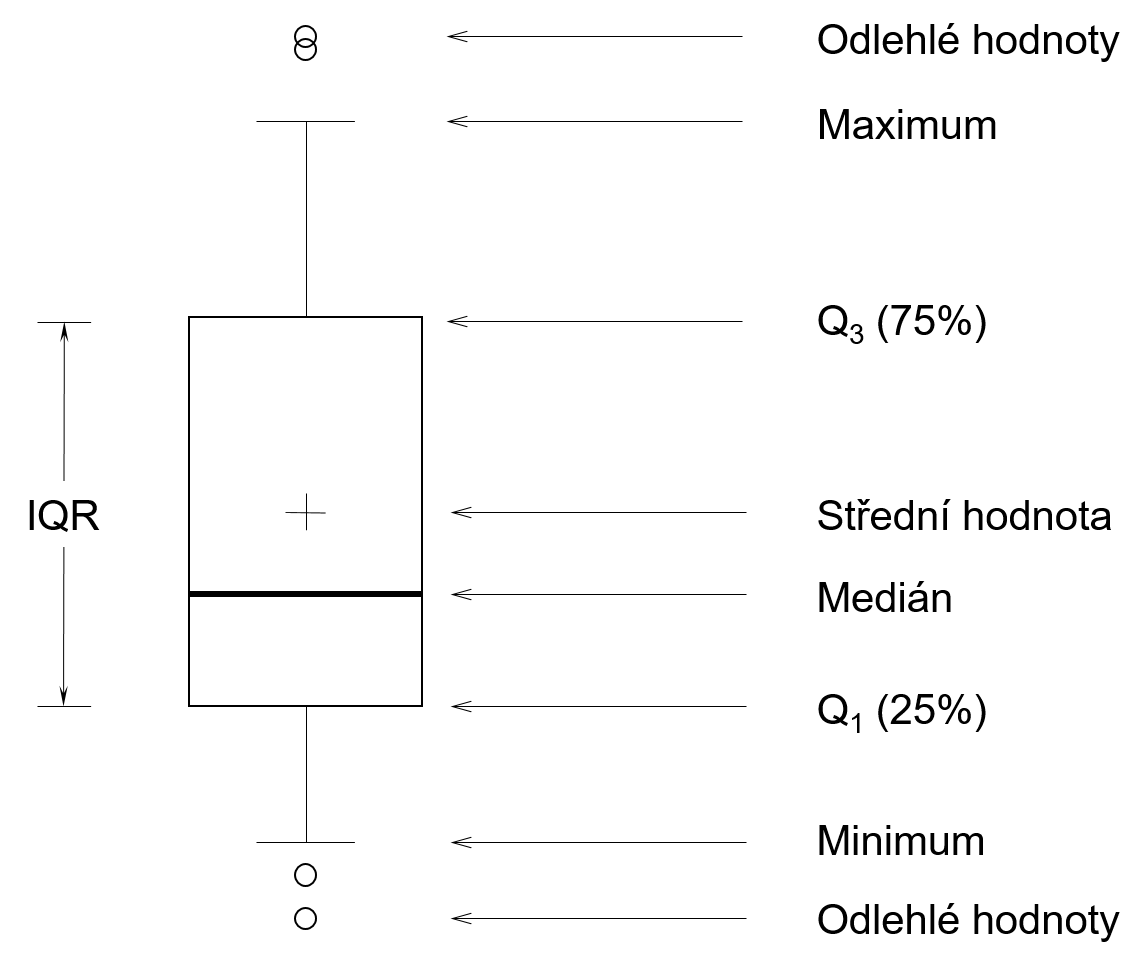
\includegraphics[width=0.65\linewidth]{fig/boxplot} 

}

\caption{\label{fig:ch2.4} Boxplot}\label{fig:boxplot_img}
\end{figure}

\newpage

\subsubsection{2.4 Sloupcový graf}\label{sloupcovy-graf}

\qquad Sloupcový graf je jedním z nejvíce používaných způsobů
vizualizace dat. Obvykle se používá pro zobrazení kvantitativních hodnot
na ose y a kvalitativních na ose x. Výška sloupců může reprezentovat jak
četnosti výskytu hodnot, tak i samotné hodnoty.(Chang 2012)

\qquad V R lze tento typ grafu vykreslit pomocí funkce
\texttt{barplot()}. V příkladu (Obrázek \ref{fig:ch2.5}) je použit data
set \texttt{mtcars}, konkretně atribut \texttt{cyl} - počet válců v
motoru.

\begin{Shaded}
\begin{Highlighting}[]
\KeywordTok{table}\NormalTok{(mtcars}\OperatorTok{$}\NormalTok{cyl)}
\end{Highlighting}
\end{Shaded}

\begin{verbatim}
## 
##  4  6  8 
## 11  7 14
\end{verbatim}

\begin{Shaded}
\begin{Highlighting}[]
\KeywordTok{barplot}\NormalTok{(}\KeywordTok{table}\NormalTok{(mtcars}\OperatorTok{$}\NormalTok{cyl))}
\end{Highlighting}
\end{Shaded}

\begin{figure}[H]

{\centering 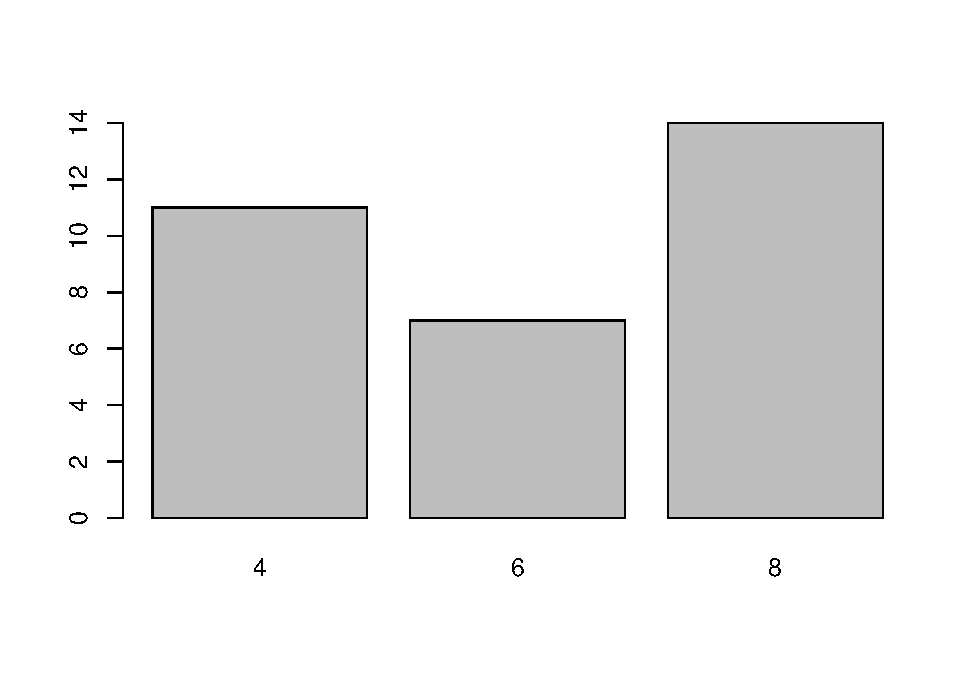
\includegraphics[width=0.55\linewidth]{BP_files/figure-latex/barplot-1} 

}

\caption{\label{fig:ch2.5} Ukázka jednoduchého sloupcového grafu}\label{fig:barplot}
\end{figure}

\hypertarget{hist}{\subsubsection{2.4.1 Histogram}\label{hist}}

\qquad Sloupcový graf s četnostmi na souvislé ose je také známý jako
histogram (Chang 2012). Četnosti mohou být absolutní či relativní.
Absolutní četnost zobrazuje počet statistických jednotek s hodnotou
znaku, který patří do určitého intervalu. Podíl příslušné četnosti a
rozsahu datového souboru se nazývá relativní četnost (Novovičová 2006).
Šířka sloupce reprezentuje jednotlivé intervaly, které mají stejnou
délku. Pro výpočet optimální délky intervalu existují různé metody.
Základní histogram se vytváří pomocí funkci \texttt{hist()} a její
atribut \texttt{breaks} udává buď hranice intervalů, jejich preferovaný
počet nebo metodu výpočtu intervalu. V R jsou vestavěny tři metody
výpočtu:

\newpage

\begin{enumerate}
\def\labelenumi{\arabic{enumi}.}
\tightlist
\item
  Sturges (Maciejewski 2011)
\end{enumerate}

\begin{Shaded}
\begin{Highlighting}[]
\KeywordTok{hist}\NormalTok{(x, }\DataTypeTok{breaks =} \StringTok{"Sturges"}\NormalTok{)}
\end{Highlighting}
\end{Shaded}

\[k=[log_2(n)]+1\] Kde \(k\) je počet intervalů a \(n\) je počet prvků
neboli počet pozorování výběru \(x\). Tato metoda je výchozí pro funkci
\texttt{hist()}.

\begin{enumerate}
\def\labelenumi{\arabic{enumi}.}
\setcounter{enumi}{1}
\tightlist
\item
  Scott (Maciejewski 2011)
\end{enumerate}

\begin{Shaded}
\begin{Highlighting}[]
\KeywordTok{hist}\NormalTok{(x, }\DataTypeTok{breaks =} \StringTok{"Scott"}\NormalTok{)}
\end{Highlighting}
\end{Shaded}

Scotovo pravidlo je následující:
\[h=\frac{3.5 \sigma}{n^{\frac{1}{3}}}\] kde \(\sigma\) je směrodatná
odchylka a \(h\) je předpokládaná šířka intervalu.

Počet intervalů může být vypočítán pomocí vztahu:
\[k=\Big[\frac{max(x)-min(x)}{h}\Big]\]

Případně oba vztahy lze shrnout do jednoho:
\[k = \Big[n^{\frac{1}{3}}{\frac{max(x)-min(x)}{3.5 \sigma}}\Big]\]

\begin{enumerate}
\def\labelenumi{\arabic{enumi}.}
\setcounter{enumi}{2}
\tightlist
\item
  Freedman--Diaconis
\end{enumerate}

\begin{Shaded}
\begin{Highlighting}[]
\KeywordTok{hist}\NormalTok{(x, }\DataTypeTok{breaks =} \StringTok{"FD"}\NormalTok{)}
\end{Highlighting}
\end{Shaded}

Freedman--Diaconisovo pravidlo pro stanovení předpokládané šířky
intervalu je:

\[h=2\frac{IQR(x)}{n^{\frac{1}{3}}}\] Po dosazení:
\[k = \Big[n^{\frac{1}{3}}{\frac{max(x)-min(x)}{2IQR(x)}}\Big]\]

kde \(IQR\) je mezikvartilové rozpětí, které definujeme jako rozdíl
třetího a prvního kvartilů.

Histogram je jedním ze standardních způsobů, používaných k odhadu tvaru
rozdělení, přesto se ale tento způsob považuje za nepřesný, vzhledem k
ovlivnění tvaru počtem použitých intervalů. Při normálním rozdělení by
měl histogram mít zvoncovitý tvar schodný s Gaussovou křivkou (Obrázek
\ref{fig:ch2.6}).

\begin{figure}[H]

{\centering 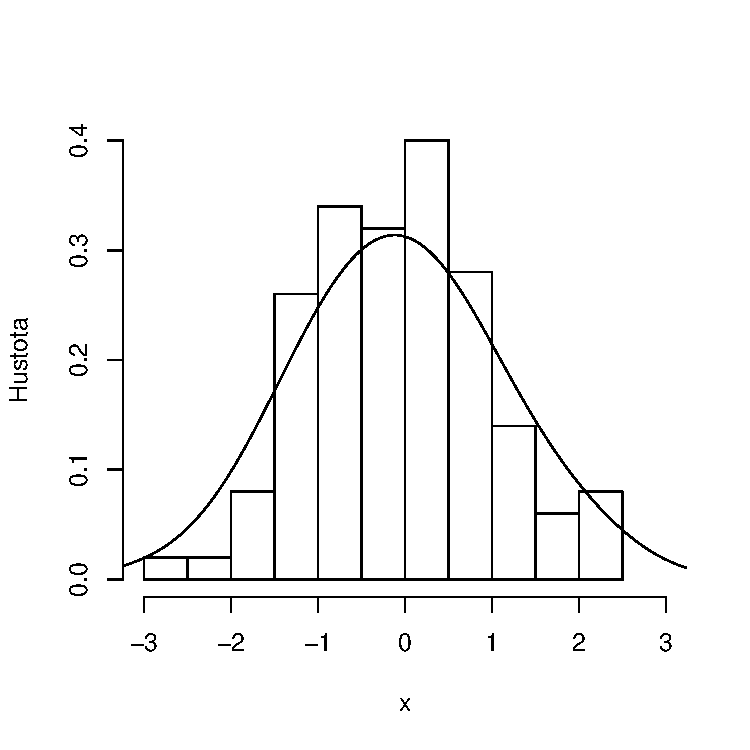
\includegraphics[width=0.6\linewidth]{BP_files/figure-latex/hist_example-1} 

}

\caption{\label{fig:ch2.6} Histogram s odhadem hustoty pravděpodobnosti}\label{fig:hist_example}
\end{figure}

\paragraph{2.4.2 Koláčový graf}\label{kolacovy-graf}

\qquad Koláčový graf představuje plný kruh (360°), který je rozdělen na
jednotlivé výseče pro znázornění číselných proporci mezi proměnnými.
Koláčový graf je tvořen transformaci skládaného sloupcového grafu do
polárního souřadnicového systému (Obrázek \ref{fig:ch2.7}) (Wilkinson
2005).

\begin{figure}[H]

{\centering 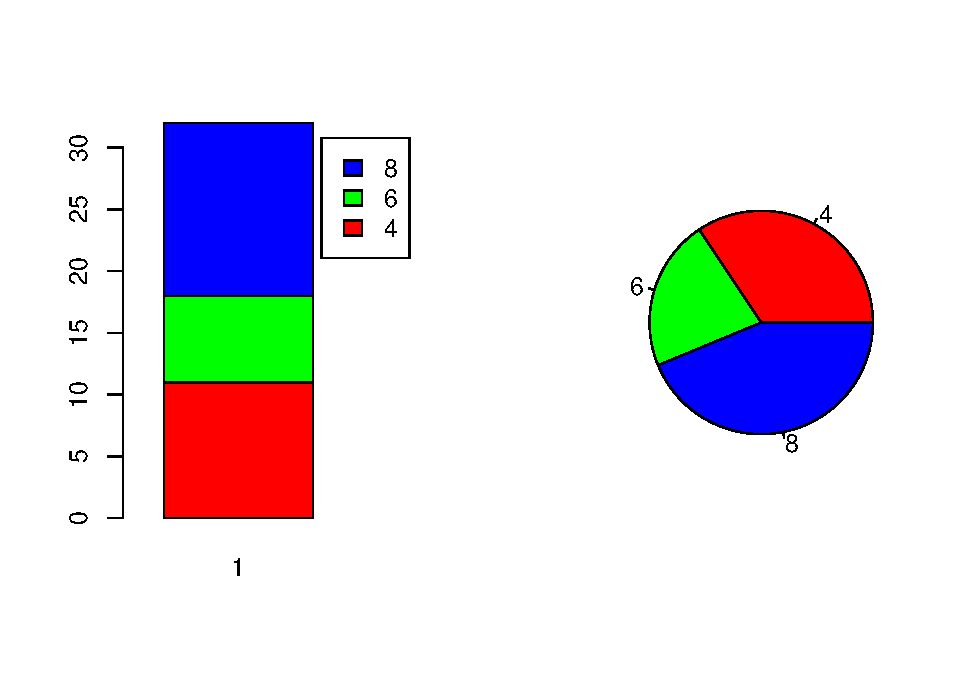
\includegraphics[width=0.65\linewidth]{BP_files/figure-latex/barplot_to_pie-1} 

}

\caption{\label{fig:ch2.7} Skládaný sloupcový graf transformovaný do polárního souřadnicového systému}\label{fig:barplot_to_pie}
\end{figure}

\qquad Jednoduché koláčové grafy se vykreslují pomoci funkci
\texttt{pie()} (Obrázek \ref{fig:ch2.8}).

\begin{figure}[H]

{\centering 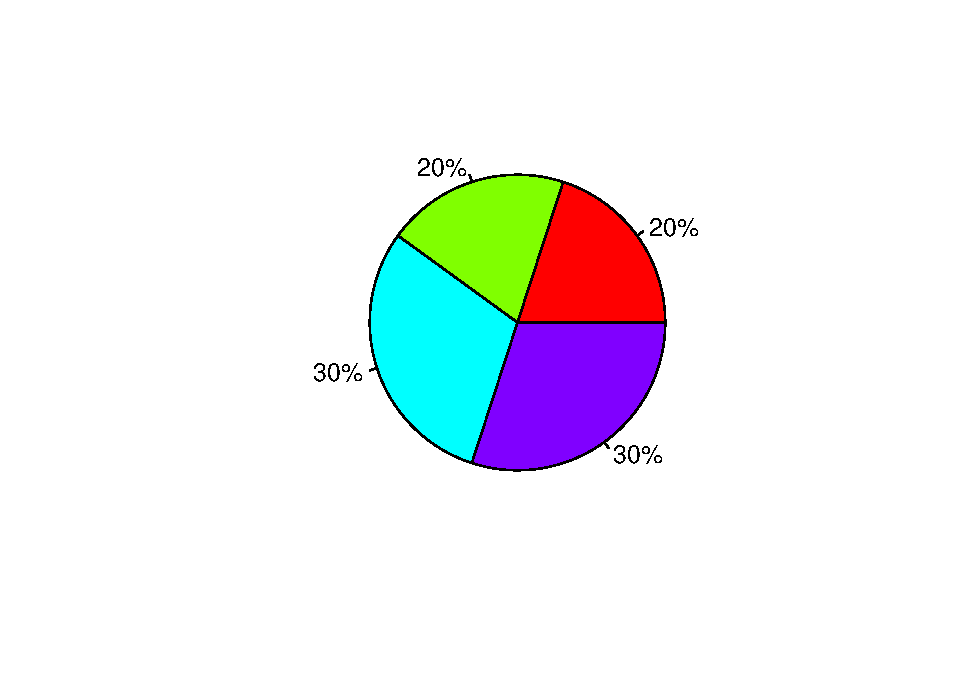
\includegraphics[width=0.65\linewidth]{BP_files/figure-latex/pie_example-1} 

}

\caption{\label{fig:ch2.8} Ukázka jednoduchého koláčového grafu}\label{fig:pie_example}
\end{figure}

\hypertarget{stem-and-leaf}{\paragraph{\texorpdfstring{2.4.3 Číslicový
histogram
(\emph{stem-and-leaf})}{2.4.3 Číslicový histogram (stem-and-leaf)}}\label{stem-and-leaf}}

\qquad Číslicový histogram, jinak známy jako \emph{stem-and-leaf plot},
podobně jako histogram pomáhá vizualizovat tvar rozdělení. Jedná se
spíše o historický typ grafu, který byl populární v osmdesátých letech,
kvůli obtížnějšímu vykreslování velkých datasetů. Vstupní údaje jsou
rozdělené vertikální linií na dva sloupce. Pravý sloupec obsahuje listy
(\emph{leaf})~-~poslední číslice po desetinné čárce a levý sloupec
obsahuje stonek (\emph{stem})~-~číslice před desetinnou čárkou. Každý
stonek je uveden pouze jednou i pokud neobsahuje žádné listy. Listy se
uvádějí od nejmenšího po největší. (Tukey 1977) Proto v příkladu
uvedeném níže je v prvním řádku stonkem číslice -2 a listy jsou číslice
9 a 2. Víme tak, že v datasetu se vyskytli čísla -2.9 a -2.2. Tento typ
grafu v~prostředí R se vykresluje pomoci funkce \texttt{stem()}:

\begin{Shaded}
\begin{Highlighting}[]
\KeywordTok{stem}\NormalTok{(x)}
\end{Highlighting}
\end{Shaded}

\begin{verbatim}
## 
##   The decimal point is at the |
## 
##   -2 | 92
##   -1 | 888755333332211100
##   -0 | 99888877666666655554433332111100
##    0 | 0011122222233334444456777788888999
##    1 | 0233445689
##    2 | 0012
\end{verbatim}

\newpage

\hypertarget{EDA}{\subsection{3 Průzkumová analýza dat}\label{EDA}}

\begin{figure}[H]

{\centering 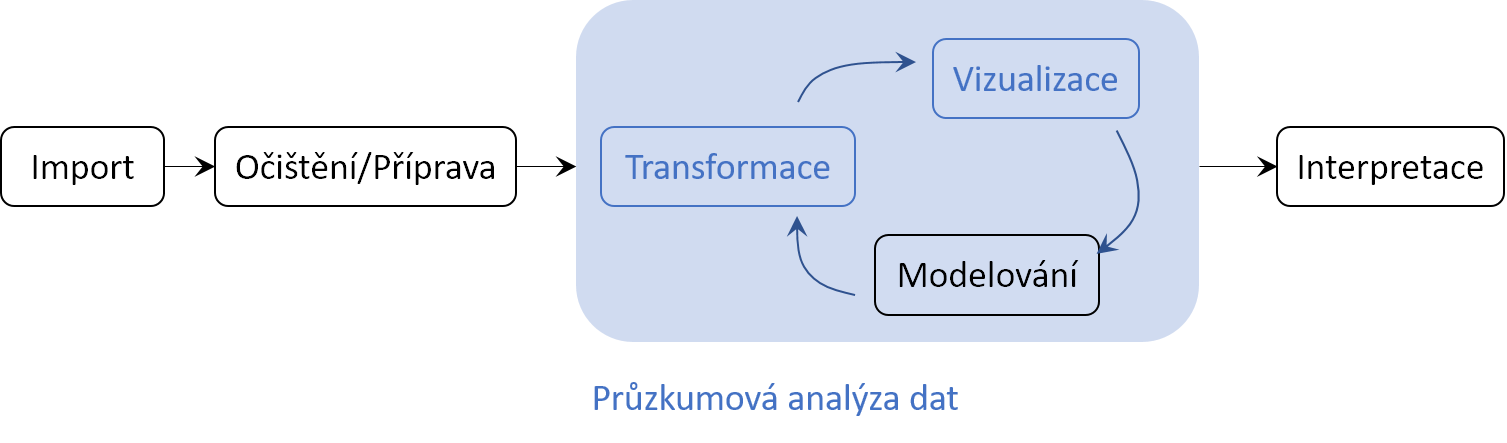
\includegraphics[width=1\linewidth]{fig/EDA_diagram2} 

}

\caption{\label{fig:ch3.1} Posloupnost datové analýzy}\label{fig:diagram_img}
\end{figure}

\qquad Úkolem průzkumové analýzy dat (\emph{Explanatory Data Analysis},
zkráceně EDA) je vizualizace a transformace dat systematickým způsobem
za účelem maximálního pochopení dat, určení vztahu mezi nimi a posouzení
jejích kvality. EDA je důležitou části datové analýzy a měla by být
jedním z jejích prvních kroků.

\qquad Zařazení průzkumové analýzy dat do procesu datové analýzy je
zobrazeno v~diagramu \ref{fig:ch3.1}. Prvním krokem datové analýzy je
\textbf{import} dat. Obecně to v tomto případě znamená nahrání
obdržených dat ze souboru či databáze do prostředí R. Bez tohoto kroku
datová analýza nemůže být vykonána. V momentě když data jsou importována
do R je vhodné je upravit do formátu vhodného pro analýzu - tzv.
\emph{tidy data} (kapitola~\protect\hyperlink{tidydata}{3.5}). Tím je
myšleno ukládání dat v konzistentní a systematické formě, odpovídající
sémantice původního datasetu. Zkrátka, očištěná (\emph{tidy}) data jsou
taková data, ve kterých sloupce odpovídají proměnným a řádky odpovídají
pozorováním.

\qquad Jakmile jsou data očištěna, je obvyklým krokem jejich
\textbf{transformace}. Transformací se rozumí omezení pozorování
(například dle zájmového území či povodí), vytváření nových proměnných
na základě již existujících, agregace (např. z denního do měsíčního
kroku), výpočet souhrnných statistik (středních hodnot, kvantilů atd.),
odstranění odlehlých pozorování a normalizace. Poté, co jsou data
očištěná a obsahují veškeré potřebné proměnné, je možné na ně aplikovat
dva nejdůležitější nástroje k~zjištění informací: vizualizaci a
modelování. Jakákoliv analýza tyto nástroje opakovaně využívá.

\qquad \textbf{Vizualizace} je schopná odhalit neočekávané chování dat a
napovědět další směr analýzy. Vizualizaci lze odhalit nevhodně zvolená
či špatně připravená data a~nekorektní dotazování. I přesto, že
vizualizace je dobrým nástrojem datové analýzy, její aplikace na větší
datasety je značně náročná a interpretace výsledků je subjektivní, tudíž
závisí na analytikovi.

\qquad \textbf{Modelování} je v rámci průzkumové analýzy dat doplňkem
vizualizace. Jedná se o zásadně matematický a výpočetní nástroj, který
se obecně hodí i na větší datasety. Téměř každý model musí splňovat své
předpoklady, které by měli být ověřeny před jejich aplikací, na rozdíl
od vizualizace, která žádné předpoklady nevyžaduje (Wickham a Grolemund
2017).

\qquad Důležitou součástí analýzy je \textbf{interpretace} výsledků a
formulace závěrů. Vyhodnocuje, jak dobře zvolený model či vizualizace
slouží k pochopení dat a jejich popisu. Je také důležité si uvědomit,
komu jsou výsledky interpretovány, kdo je cílová skupina. Dobře
provedené grafické výstupy podložené jejich správnou interpretaci jsou
jedním z nejlepších způsobů prezentace dat.

\qquad Průzkumová analýza dat není specifikována jako konkrétní soubor
pravidel a~postupů, ale jako přístup k analýze dat. Obvykle zahrnuje
následující kroky:

\begin{itemize}
\tightlist
\item
  Vyhledávání vybočujících (odlehlých) pozorování
\item
  Náhrada chybějících hodnot
\item
  Transformace dat
\item
  Změny typu proměnných
\item
  Ověřování normality
\end{itemize}

\subsubsection{3.1 Odlehlá pozorování}\label{odlehla-pozorovani}

\qquad Odlehlá pozorování (\emph{outliers}) jsou významně odlišná vůči
ostatním hodnotám datasetu. Definice toho, jak moc odlišná taková
pozorování mají být je dáno analytikem na základě konkretního datasetu a
kontextu problematiky. Tato pozorování mohou být indikátorem chybných
dat nebo vzácných událostí. Důvody proč se tato pozorování vyskytují by
měli být pečlivě zkoumány. Dále je důležité posoudit, jak je jimi
výsledek analýzy ovlivněn, případně zdali je předpoklady metody
připouštějí.

\qquad Hledání odlehlých, vybočujících, pozorování a jiných anomálií pro
jednotlivé veličiny lze provést graficky například pomoci boxplotu (viz
sekce \protect\hyperlink{boxplot}{2.3.2}), bodových grafů
(\protect\hyperlink{scatterplot}{2.1}) nebo číslicových histogramů
(\protect\hyperlink{stem-and-leaf}{2.4.3}). Dají se také vypočítat
pomocí různých statistik, například metodou \emph{jackknife}, která je
popsána v následující kapitole (\protect\hyperlink{jackknife}{3.1.1}). V
momentech, kdy je vizualizace obtížná (velké datasety, větší množství
navzájem se ovlivňujících proměnných, atd.), využívají se nástroje
vícerozměrné, například Mahalanobisovy vzdálenosti
(\protect\hyperlink{mbdist}{3.1.2}), \emph{leverages}
(\protect\hyperlink{leverages}{3.1.3}) a další.

\hypertarget{jackknife}{\paragraph{\texorpdfstring{3.1.1
\emph{Jackknife}}{3.1.1 Jackknife}}\label{jackknife}}

\qquad Metoda byla původně představená Johnem W. Tukeyem v roce 1958 v
\enquote{\emph{The Annals of Mathematical Statistic}} (Tukey 1958) a
jedná se o speciální případ metody \emph{bootstrap} (více o metodě B.
Efron a R. Tibshirani v \enquote{\emph{An Introduction to the
Bootstrap}} (Efron a Tibshirani 1994)).

\qquad Postup metody \emph{jackknife} je založen na celkem jednoduché
myšlence. Zjišťují se souhrnné statistiky podsouborů (\emph{Jackknife
Samples}), které se vytvářejí postupným vypouštěním jednotlivých
pozorování z původního datasetu. Jinými slovy existuje \(n\)~unikátních
Jackknife podsouborů a \(i\)-tý Jackknife podsoubor je definován jako
vektor.

\qquad Pomocí porovnání souhrnných statistik původního datasetu a
vytvořených Jackknife podsouborů se odhadne vliv jednotlivých pozorování
na původní dataset. Jedna ze souhrnných statistik, kterou lze použít je
střední hodnota \(\bar{x}\). Pro původní dataset obsahující \(n\)
pozorování lze střední hodnotu odhadnout dle vzorce
\(\bar{x} = \frac{1}{n} \sum \limits_{i=1}^{n} \bar{x}_i\). Střední
hodnota Jackknife podsouborů se vyhodnotí následovně:
\[\bar{x}_i = \frac{1}{n-1} \sum \limits_{j=1, j \neq i}^{n} x_j, \quad \text{kde } i=1,\dots,n.\]
Porovnání lze provést dle vzorce
\(\textit{Var}(\bar{x}) = \frac{n-1}{n} \sum \limits_{i=1}^{n}(\bar{x}_i - \bar{x})^2\),
kde \(\textit{Var}(\bar{x})\) je odhad rozptylu, který indikuje, jak moc
jednotlivá pozorování ovlivňují dataset, tj. přítomnost odlehlých
pozorování. Metoda může být také použita k odhadu skutečné, neovlivněné
střední hodnoty datasetu. (McIntosh 2016)

\hypertarget{mbdist}{\paragraph{3.1.2 Mahalanobisovy
vzdálenosti}\label{mbdist}}

\qquad K měření vzdálenosti mezi objekty se často používá euklidovská
vzdálenost. Euklidovská vzdálenost je jednoduchá na výpočet a
interpretaci, ale není schopná brát v úvahu vztahy mezi daty. Proto je v
řádě případů vhodné použít mahalanobisovou vzdálenost. Je definovaná
matice \(\bm{X}(n \times p)\), obsahující \(n\) objektů \(\bm{x}_i\) a
\(p\) proměnných. Euklidovská vzdálenost mezi vektorem \(i\)-tého řádku
\(\bm{x}_i (1 \times p)\) této matice a vektoru středních hodnot
\(\bar{\bm{x}} (1 \times p)\) se spočítá jako
\[ED_i = \sqrt{(\bm{x}_i - \bar{\bm{x}})(\bm{x}_i - \bar{\bm{x}})^T}, \quad \text{pro } i = 1,\dots,n\]
zatímco mahalanobisova vzdálenost se spočítá jako
\[MD_i = \sqrt{(\bm{x}_i - \bar{\bm{x}}) \bm{C}^{-1}_x (\bm{x}_i - \bar{\bm{x}})^T}, \quad \text{pro } i = 1,\dots,n\]
kde \(\bm{C}_x\) je kovarianční matice. (De Maesschalck et al. 2000)

\qquad Na obrázku \ref{fig:ch3.2} jsou znázorněny elipsy
mahalanobisových vzdáleností, kde každá elipsa představuje vzdálenost od
průměru. Z tohoto je zřejmé, že vzdálenost roste pomaleji ve směru
korelace. Pozorování, které je výrazně vzdáleno od středu, ale leží ve
směru závislosti, má nižší mahalanobisovou vzdálenost než pozorování,
které je stejně vzdáleno od středu, ale neleží ve směru závislosti. Tato
vlastnost mahalanobisových vzdálenosti umožňuje identifikaci odlehlých
pozorování.

\qquad Metoda byla představena P.C. Mahalanobisem v roce 1936 ve článku
\emph{\enquote{On the Generalized Distance in Statistics}} (Mahalanobis
1936). Mahalanobisové vzdálenosti se používají nejenom k nalezení
odlehlých pozorování, ale i ke zkoumání reprezentativity mezi dvěma data
sety, aplikuje se v algoritmu \(k\)-nejbližších sousedů, v diskriminační
analýze a má mnoho dalších uplatnění.

\begin{figure}[H]

{\centering 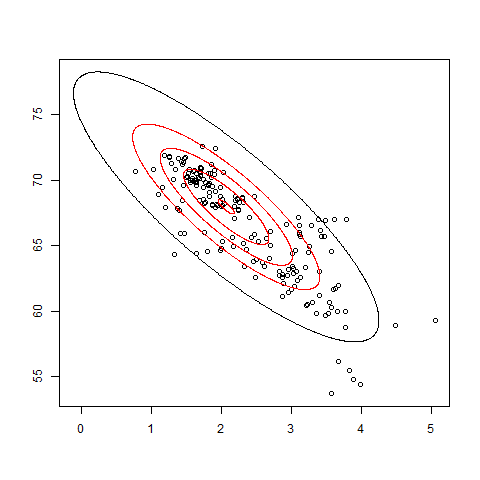
\includegraphics[width=0.65\linewidth]{fig/mahalanobis} 

}

\caption{\label{fig:ch3.2} Mahalanobisovy vzdálenosti}\label{fig:mbdist_img}
\end{figure}

\hypertarget{leverages}{\paragraph{3.1.3 Leverages}\label{leverages}}

\qquad Leverage (případně též efekt, vliv nebo projekční \(h\) prvek) se
používá v regresní analýze k měření velikosti vlivu pozorování na
regresní odhad. Princip metody spočívá v kontrole diagonálních prvků
projekční matice \(\bm{H}\), která je produktem metody nejmenších
čtverců a je definována
\[\bm{H} = \bm{X}(\bm{X}^T\bm{X})^{-1}\bm{X}^T.\] Model lineární regrese
může být zapsán následovně:
\[\bm{y} = \bm{X \beta} + \bm{\varepsilon},\] kde vektor vysvětlované
proměnné je \(\bm{y}\), matice vysvětlujících proměnných je \(\bm{X}\),
vektor regresních koeficientů, který je odhadován, je \(\bm{\beta}\) a
vektor náhodné složky je \(\bm{\varepsilon}\). Metoda nejmenších čtverců
poskytuje řešení regresních rovnic:
\[\bm{\beta} = (\bm{X}^T\bm{X})^{-1} \bm{X}^T \bm{y}.\] Lze dosadit:
\[\hat{\bm{y}} = \bm{X \beta} = \bm{X}(\bm{X}^T\bm{X})^{-1} \bm{X}^T \bm{y}.\]
Výsledný vektor má tvar \(\hat{\bm{y}} = \bm{Hy}\), kde \(\bm{H}\) je
projekční matice. (Cardinali 2014)

\subsubsection{3.2 Náhrada chybějících
pozorování}\label{nahrada-chybejicich-pozorovani}

\qquad Problém chybějících pozorování spočívá v neschopnosti jejich
zpracovávání některými metodami. Takové hodnoty lze vynechat nebo
doplnit (nahradit) jednou z řady metod. Vynechání hodnot vede k
nežádoucímu zmenšení datasetu, proto je výhodnější chybějící údaje
doplnit. Nejednodušším nástrojem pro náhradu chybějících hodnot je
aritmetický průměr příslušné proměnné. Tento způsob může vést ke
zkresleným odhadům (neplatí-li předpoklad, že chybějící údaje jsou zcela
náhodné) a podhodnocuje variabilitu a kovarianci datasetu, a proto se
nedoporučuje v případě vyššího podílu chybějících údajů. Další možnou
metodou je náhrada náhodným číslem generovaným z příslušného rozdělení
(parametry jsou odhadnuty z výběru). V tomto případě se respektuje
variabilita datasetu, ale nerespektuje se jeho kovariance. Chybějící
údaje lze také odvodit pomocí známých hodnot na základě pomocné
jednoduché lineární regresní funkce. Tato metoda respektuje nejenom
variabilitu vzorku, ale i jeho korelační strukturu. (Pecáková 2014)

\subsubsection{3.3 Transformace dat}\label{transformace-dat}

\qquad Jedním z cílů transformace dat je dosažení srovnatelnosti
proměnných: sjednocení měřítka, variace a typu proměnných. Hlavním
využitím je splnění podmínek vyžadovaných metodami, například podmínky
normality, kde je snaha převést data na normální rozdělení, snížení
vlivu rušivých proměnných (odlehlých hodnot) atd. (Hebák et al. 2007).
Rozdělujeme transformaci lineární (centrování, normování) a~nelineární
(plynoucí z typu a charakteru dat).

\qquad Lineární transformace zachovává lineární vztahy mezi proměnnými.
Jedním z~příkladů takovéto úpravy dat je metoda centrování, která se
používá u vícerozměrných analýz. Podstata metody spočívá v zachování
měřítka vzorku při změně hodnot: od původních hodnot se odečítá průměr
proměnné (od prvků sloupce se odečte jejich sloupcový průměr), průměry
získaných nových proměnných se tudíž rovnají nule. Toto lze zapsat
následovně: \[v_{ij} = x_{ij} - \bar{x}_j\] Vektor průměrů
\(\bar{\bm{v}}\) je nulový, kovariance a korelace proměnných zůstává
nezměněna. (Hebák et al. 2007) Další často využívanou metodou je metoda
normalizace dat. Tato metoda transformuje měřítka vzorků pro možnost
jejich porovnání (eliminuje jednotky měření), po úpravě střední hodnota
vzorku tedy odpovídá nule a směrodatná odchylka jedničce.
\[z_{ij} = \frac{x_{ij} - \bar{x}_j}{\sigma(x_j)}\] \(\sigma(x_j)\) je
směrodatná odchylka sloupce proměnné, vektor průměrů \(\bar{\bm{z}}\) je
nulový a~kovariance vektoru nových proměnných se shoduje s korelací
původního vektoru~(Abdi a Williams 2010).

\qquad Nelineární transformace vyplývá z typu dat a mění (snižuje či
zvyšuje) lineární vztahy mezi proměnnými a to znamená, že nezachovává
korelaci mezi nimi. Pokud data mají charakter absolutní četnosti,
používá se odmocninová transformace \(X^{\prime} = \sqrt{X}\), pokud
odpovídají log-normálnímu rozdělení, používá se logaritmická
transformace \(X^{\prime} = \log_{10}X\) atd. Logaritmus náhodné
veličiny s log-normálním rozdělením má normální rozdělení (viz obrázek
\ref{fig:ch3.3}). Logaritmická transformace může být použita pouze u
nezáporných rozdělení. (Zumel a Mount 2014) (Kutner et al. 2004)

\begin{figure}[H]

{\centering \includegraphics[width=0.82\linewidth]{BP_files/figure-latex/lognormal_to_normal-1} 

}

\caption{\label{fig:ch3.3} Log-normální rozdělení transformováné na normální rozdělení}\label{fig:lognormal_to_normal}
\end{figure}

\hypertarget{normtests}{\subsubsection{3.4 Ověřování
normality}\label{normtests}}

\qquad Důležitým aspektem popisu proměnné je tvar jejího rozdělení,
který udává četnosti hodnot z různých rozsahů proměnné. Většina
statistických testů a metod se zakládá na předpokladu, že proměnná má
normální rozdělení. Z tohoto důvodu je vhodné ověřovat normalitu
rozdělení analyzovaného vzorku.

\qquad Zjistit zda-li vzorek pochází z normálního rozdělení lze
grafickým posouzením nebo pomocí testů normality. Mezi nástroje
grafického posouzení normality se řadí histogram rozdělení četnosti
(kapitola \protect\hyperlink{hist}{2.4.1}), graf výběrové distribuční
funkce (\protect\hyperlink{distribution}{2.3}), Q-Q graf a P-P graf
(\protect\hyperlink{qqpp}{2.3.1}). Vztah hustoty rozdělení a Q-Q grafu
je znázorněn na obrázku \ref{fig:ch3.4}. Dále existuje řada testů
normality, zde jsou popsány testy Shapiro-Wilk (SW) a Jarqua-Bera (JB).

\begin{figure}[H]

{\centering \includegraphics[width=0.95\linewidth]{BP_files/figure-latex/density_qq_plot-1} 

}

\caption{\label{fig:ch3.4} Vztah hustoty rozdělení a Q-Q grafu pro různá narušení normality}\label{fig:density_qq_plot}
\end{figure}

\qquad Shapiro-Wilk test byl poprvé představen v roce 1965 S. S.
Shapirem a M. Wilkem (SHAPIRO a WILK 1965). Metoda dokáže pracovat se
vzorky velikosti 12 až 5000 pozorování. Nulová hypotéza tohoto testu
předpokládá, že vzorek má normální rozdělení. Pokud je \(p\)-hodnota
menší, než zvolená hladina významnosti, nulová hypotéza se zamítá,
jinými slovy vzorek pravděpodobně nemá normální rozdělení. Statistika
testu vypadá následovně:
\[W = \frac{\big(\sum \limits^n_{i=1} a_i x_{(i)}\big)^2}{\sum \limits^n_{i=1}(x_i - \bar{x})^2},\]
kde \(x_{(i)}\) je \(i\)-tý nejmenší prvek (statistika \(i\)-tého řádu),
\(\bar{x}\) je průměr vzorku, \(n\) je počet pozorování. Kritické
hodnoty pro tento test jsou tabelovány.

\qquad Jarqua-Bera test závisí na koeficientech šikmosti a špičatosti.
Statistika JB testu může být zapsána:
\[T = n \bigg( \frac{(\sqrt{b_1})^2}{6} + \frac{(b_2 - 3)^2}{24} \bigg),\]
kde \(n\) je velikost vzorku, \(\sqrt{b_1}\) je koeficient šikmosti
vzorku a \(b_2\) je koeficient špičatosti. \(T\) statistika má přibližně
chi-kvadrát rozdělení s dvěma stupni volnosti. Nulová a~alternativní
hypotéza se schoduje s SW testem. Používá se pro větší datasety nad 2000
pozorování. (Öztuna et al. 2006)

\hypertarget{tidydata}{\subsubsection{3.5 Tidy data}\label{tidydata}}

\qquad Přípravou dat pro průzkumovou analýzu a vizualizaci se zabýval
například Hadley Wickham ve svém članku \emph{Tidy data} z roku 2014
(Wickham 2014). V tomto článku uvádí standardy, koncepty, základní
metody a nástroje pro jejich přípravu. Hlavním cílem konceptu \emph{tidy
dat} je, aby každá proměnná odpovídala sloupci, každé pozorování
odpovídalo řádku a každá hodnota byla uložena ve vlastní buňce (viz
obrázek \ref{fig:ch3.5}).

\begin{figure}[H]
      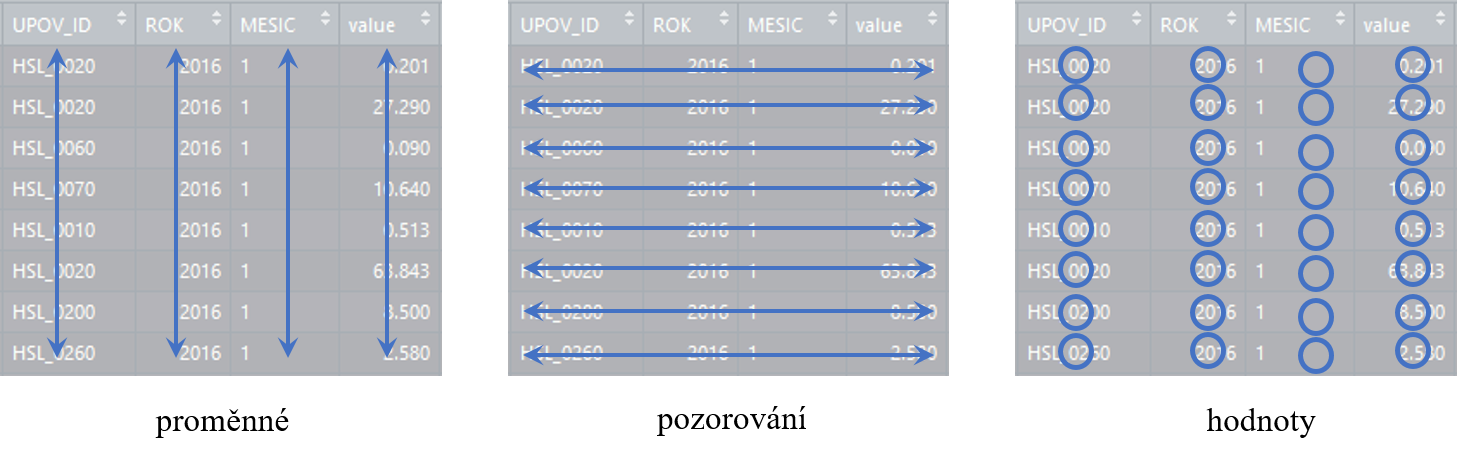
\includegraphics[width=\textwidth]{fig/tidy}
      \caption{Tří základní pravidla pro \textit{tidy data}.}
      \label{fig:ch3.5}
\end{figure}

\qquad Mezi nástroje pro \emph{tidy data} patří R balíčky:
\texttt{tidyr}, \texttt{plyr} a \texttt{dplyr}. \texttt{tidyr} (tidyr
{[}vid. 17.4.2018{]}) je balíček vytvořený konkrétně pro tvorbu
\emph{tidy dat} a to pomocí dvou hlavních funkcí \texttt{gather()} a
\texttt{spread()}. Funkce \texttt{gather()} převádí vícesloupcová
(víceproměnná) data do formátu \enquote{klíč-hodnota} resp. do
\enquote{dlouhého} formátu, zatímco funkce \texttt{spread()} číní přesný
opak a tedy převádí data do takzvaného \enquote{širokého} formátu.
Rozdíl mezi \enquote{širokým} a \enquote{dlouhým} formátem dat je
ilustrován v tabulkách \ref{tab3} a \ref{tab4}. Balíček \texttt{plyr}
(plyr {[}vid. 17.4.2018{]}) je soubor nástrojů sloužící k rozdělení
velkých souborů dat do stejnorodých menších podsouborů. S jednotlivými
podsoubory lze libovolně manipulovat (počítat souhrnné statistiky,
standardizovat hodnoty, atd.) a~následně lze výsledky pomocí
\texttt{plyr} funkcí kombinovat zpět do jednoho souboru. \texttt{dplyr}
(dplyr {[}vid. 17.4.2018{]}) je další verzí balíku \texttt{plyr}
představenou Hadley Wickhamem v~roce 2014. Balíček poskytuje sadu
nástrojů pro efektivní manipulaci s~datasety v~R, je rychlejší a
jednodušší na použití. \vspace*{-0.9cm}

\begin{minipage}[c]{0.48\textwidth}
\begin{table}[H]
\begin{tabular}{|ccccc|}
  \hline
DTM & P & E & R & T \\ 
  \hline
1948-01-01 & 5.86 & 1.14 & 1.54 & 15.48 \\ 
   \hline
\end{tabular}
\vspace*{1.5mm}
\caption{Soubor v "širokém" formátu.}
\label{tab3}
\vspace*{12mm}
\end{table}
\end{minipage}\begin{minipage}[c]{0.14\textwidth}

\includegraphics[width=\textwidth]{fig/blank_v}
\end{minipage}\begin{minipage}[c]{0.39\textwidth}
\begin{table}[H]
\begin{tabular}{|ccc|}
  \hline
DTM & variable & value \\ 
  \hline
1948-01-01 & P & 5.86 \\ 
1948-01-01 & E & 1.14 \\ 
1948-01-01 & R & 1.54 \\ 
1948-01-01 & T & 15.48 \\ 
   \hline
\end{tabular}
\caption{Soubor v "dlouhém" \\ formátu.}
\label{tab4}
\end{table}
\end{minipage}

\newpage

\hypertarget{pokrocila}{\subsection{4 Pokročilá vizualizace v
R}\label{pokrocila}}

\qquad Před samotným popisem nástrojů pro pokročilou vizualizaci je
vhodné vysvětlit pár důležitých pojmů, které jsou v této kapitole dále
používány. Tyto pojmy se tykají vizualizace pouze okrajově, avšak v
praxi jsou často využívány právě v kombinaci s~vizualizačními
prostředky.

\qquad \texttt{R\ Studio} je volně přístupné open source vývojové
prostředí (\emph{Integrated Development Environment} neboli \emph{IDE})
pro programovací jazyk R. Společnost \texttt{R\ Studio} bylo založeno v
roce 2008 J.J. Allairem a v současnosti je hlavním vývojářem Hadley
Wickham. Hlavním produktem společnosti je IDE Rstudio - jedná se o
vývojové prostředí obsahující veškeré potřebné nástroje pro práci s R
(RStudio {[}vid. 16.4.2018{]}). Společnost \texttt{R\ Studio} kromě
vývoje samotného \emph{IDE} vyvíjí jedny z nepopulárnějších balíčků
(např. \texttt{ggplot2}, \texttt{tidyverse}, \texttt{rmakrdown},
\(\dots\)) a servery pro \texttt{Shiny}. \texttt{R\ Studio} je dostupné
ve verzi zdarma, která poskytuje všechny klíčové funkce a v komerční
verzi, pro kterou je navíc dostupná oficiální podpora (RStudio {[}vid.
16.4.2018{]}).

\qquad \texttt{R\ Markdown} je založen na značkovacím jazyku
\texttt{Markdown} a slouží pro úpravu prostého textu a jeho následný
převod do HTML, PDF, MS Word a dalších formátů a to rovnou z prostředí R
(rmarkdown {[}vid. 16.4.2018{]}). Balíček využívá univerzální nástroj
pro převod souborů \texttt{pandoc}, díky čemuž lze v rámci souboru
používat \LaTeX ~příkazy pro pokročilou úpravu PDF výstupů. Dále díky
balíčku \texttt{knitr} je umožněna integrace R kódu do výstupů. Více o
\texttt{R\ Markdown} píše autor a spoluautor těchto balíčků Yihui Xie
například (Xie 2018) a (Xie 2015).

\hypertarget{baseviz}{\subsubsection{4.1 Balíčky pro vizualizaci
dat}\label{baseviz}}

\qquad Vestavěný balíček \texttt{base} byl vyvinut Rossem Ihaka na
základě zkušeností s~implementací grafických ovladačů do S (předchůdce
R). Grafy v \texttt{base} mají charakter grafů na papíře: stávající
obsah nelze modifikovat ani odstranit. Do grafu lze přidávat potřebné
prvky, které jsou vykreslovány na povrch grafu a po vykreslení nemohou
být dále měněny. V \texttt{base} neexistuje jiná uživateli přístupná
reprezentace, než ta, co se objeví na obrazovce (není např. možné uložit
graf jako proměnnou). \texttt{base} obsahuje nástroje pro kreslení jak
základních, tak i kompletních grafik. Funkce tohoto balíčku jsou obecně
rychlé, ale mají omezené možnosti. Vykreslení základních grafů v R je
popsáno v kapitole \protect\hyperlink{base}{2}.

\qquad Mimo \texttt{base} má uživatel možnost využít rozsáhlou nabídku
dalších balíčků. Následující kapitoly obsahují krátký popis vybraných,
široce využívaných, balíčku (\texttt{grid}, \texttt{lattice},
\texttt{ggplot2}). V R existuje mnoho dalších balíčků, například
\texttt{vcd}, \texttt{plotrix} a \texttt{gplot}, které implementují
speciální grafiku, avšak žádný z nich neposkytuje rámec pro tvorbu
statistických grafů. Pro instalaci balíčků se používá příkaz
\texttt{install.packages()}. Komplexní zdroj, uvádějící všechny grafické
funkce dostupné v ostatních balíčcích vyvinutých komunitou lze nalézt na
stránce \mbox{http://cran.r-project.org/web/views/Graphics.html}.
(Wilkinson 2005)

\paragraph{\texorpdfstring{4.1.1 \texttt{grid}}{4.1.1 grid}}\label{grid}

\qquad \texttt{grid} je alternativou jednoduché grafiky z \texttt{base}
s rozsáhlejšími možnosti pro úpravu grafu. Vývoj balíčku začal v roce
2000. Autorem je Paul Murrell a balíček vznikl na základě jeho doktorské
práce \emph{Investigations in Graphical Statistics} z roku 1998 (Murrell
1998). Grafické objekty v \texttt{grid} mohou být reprezentovány
nezávislé na grafu a později upraveny. Systém \emph{viewport}ů (každý
obsahuje vlastní souřadnicový systém) usnadňuje rozvržení komplexní
grafiky. Balíček umožňuje vykreslení jednotlivých výkresů, avšak nemá
explicitní nástroje pro tvorbu statistických grafů (Murrell 2003).

\hypertarget{lattice}{\paragraph{\texorpdfstring{4.1.2
\texttt{lattice}}{4.1.2 lattice}}\label{lattice}}

\qquad Deepayanem Sarkarem vyvinutý balíček \texttt{lattice} používá
grafiku \texttt{grid} k implementaci Clevelandova \emph{trellis}
grafického systému (viz kapitola \protect\hyperlink{cleveland}{1.2.2}),
což vedlo k~značnému vylepšení grafiky oproti \texttt{base}. Pomocí
\texttt{lattice} lze jednoduše vykreslit \emph{trellis} graf a některé
detaily výkresu, jako například legenda, se vytváří automaticky. Avšak
\texttt{lattice} postrádá formální model, což může ztížit jeho
rozšíření. Tento balíček je dostačující pro typické grafické potřeby a
je dostatečně flexibilní i pro zvládnutí většiny nestandardních
požadavků.

\hypertarget{ggplot}{\paragraph{\texorpdfstring{4.1.3
\texttt{ggplot2}}{4.1.3 ggplot2}}\label{ggplot}}

\qquad Balíček \texttt{ggplot2} byl vyvinut v roce 2005 Hadley Wickhamem
na základě \emph{The Grammar of Graphics} Lelanda Wilkinsona (Wilkinson
2005). \texttt{ggplot2} přebírá přednosti balíčků \texttt{base} a
\texttt{lattice} a vylepšuje je silným základním modelem, který
podporuje tvorbu libovolného statistického grafu založeného na
principech popsaných v kapitole \protect\hyperlink{gg}{1.3}. Silný
základní model \texttt{ggplot2} umožňuje popsat širokou škálu grafiky
pomocí kompaktní syntaxe a nezávislé komponenty zjednodušují rozšíření.
Obdobně jako \texttt{lattice}, využívá \texttt{ggplot2} mřížky k
vykreslení grafiky, což znamená, že umožňuje úpravu vzhledu na mnohem
nižší úrovni.

\qquad Jako ukázku lze předvést graf vykreslený pomocí různých balíčků
(obrázky \ref{fig:ch4.1a}, \ref{fig:ch4.1b}, \ref{fig:ch4.1c}). V
představeném kódu byly použity denní časové řady srážek z roku 2010
v~oblasti povodí Labe od pramene po Svatopetrský potok včetně. ID tohoto
útvaru povrchových vod je \texttt{HSL\_0010}. \texttt{DTM} odpovídá datu
v denním kroku a \texttt{P} odpovídá úhrnu srážek v milimetrech. Každý
balíček má přednastavený počáteční vzhled, který lze upravovat dle
požadavků, avšak pro tuto ukázku bylo ponecháno základní nastavení.

\begin{Shaded}
\begin{Highlighting}[]
\KeywordTok{plot}\NormalTok{(HSL_}\DecValTok{0010}\OperatorTok{$}\NormalTok{DTM, HSL_}\DecValTok{0010}\OperatorTok{$}\NormalTok{P, }\DataTypeTok{type =} \StringTok{"l"}\NormalTok{, }
                               \DataTypeTok{xlab =} \StringTok{"DTM"}\NormalTok{, }\DataTypeTok{ylab =} \StringTok{"P"}\NormalTok{,}
                               \DataTypeTok{main =} \StringTok{"`base`"}\NormalTok{)}
\end{Highlighting}
\end{Shaded}

\begin{figure}[H]
      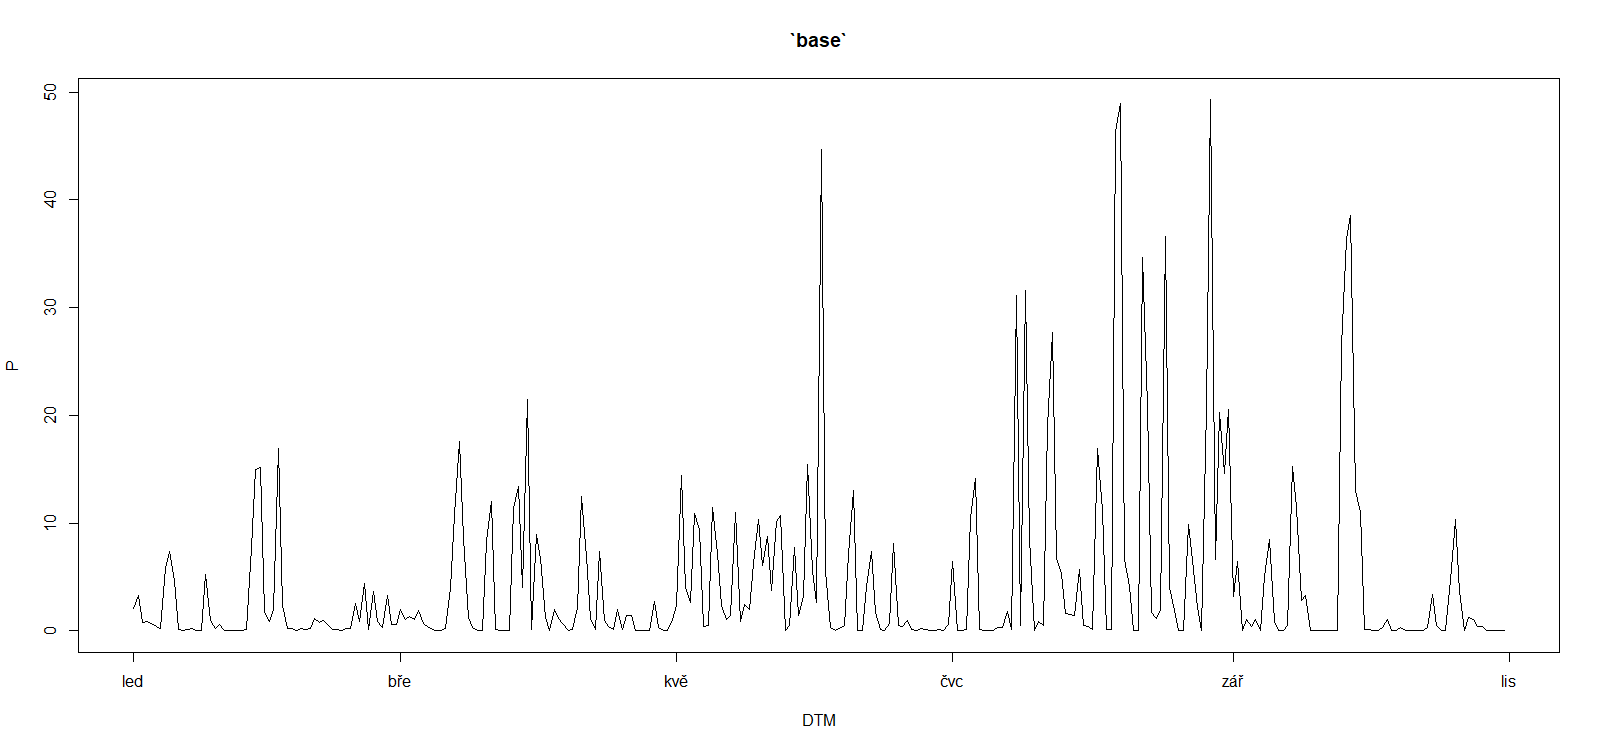
\includegraphics[width=\textwidth]{fig/1base}
      \caption{Časová řada srážek na zvoleným povodí v roce 2010, \texttt{base}}
      \label{fig:ch4.1a}
\end{figure}

\begin{Shaded}
\begin{Highlighting}[]
\KeywordTok{xyplot}\NormalTok{(P}\OperatorTok{~}\NormalTok{DTM, }\DataTypeTok{data =}\NormalTok{ HSL_}\DecValTok{0010}\NormalTok{, }\DataTypeTok{type =} \StringTok{"l"}\NormalTok{, }
                               \DataTypeTok{xlab =} \StringTok{"DTM"}\NormalTok{, }\DataTypeTok{ylab =} \StringTok{"P"}\NormalTok{, }
                               \DataTypeTok{main =} \StringTok{"`lattice`"}\NormalTok{ ,)}
\end{Highlighting}
\end{Shaded}

\begin{figure}[H]
      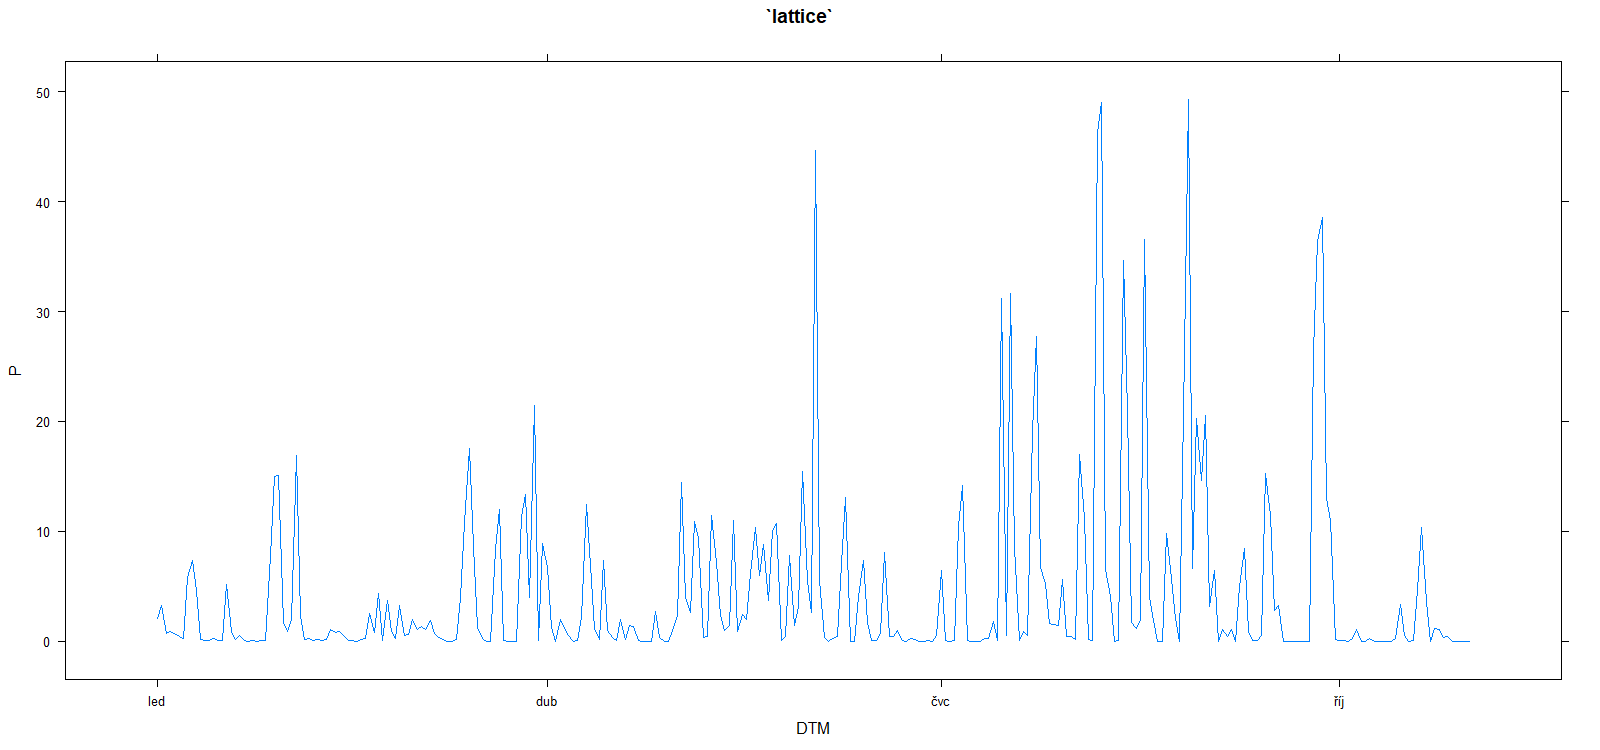
\includegraphics[width=\textwidth]{fig/2lattice}
      \caption{Časová řada srážek na zvoleným povodí v roce 2010, \texttt{lattice}}
      \label{fig:ch4.1b}
\end{figure}

\begin{Shaded}
\begin{Highlighting}[]
\KeywordTok{ggplot}\NormalTok{(}\DataTypeTok{data=}\NormalTok{HSL_}\DecValTok{0010}\NormalTok{, }\KeywordTok{aes}\NormalTok{(DTM,P)) }\OperatorTok{+}\StringTok{ }
\StringTok{  }\KeywordTok{geom_line}\NormalTok{() }\OperatorTok{+}\StringTok{ }
\StringTok{  }\KeywordTok{labs}\NormalTok{(}\DataTypeTok{title =} \StringTok{"`ggplot2`"}\NormalTok{)}
\end{Highlighting}
\end{Shaded}

\begin{figure}[H]
      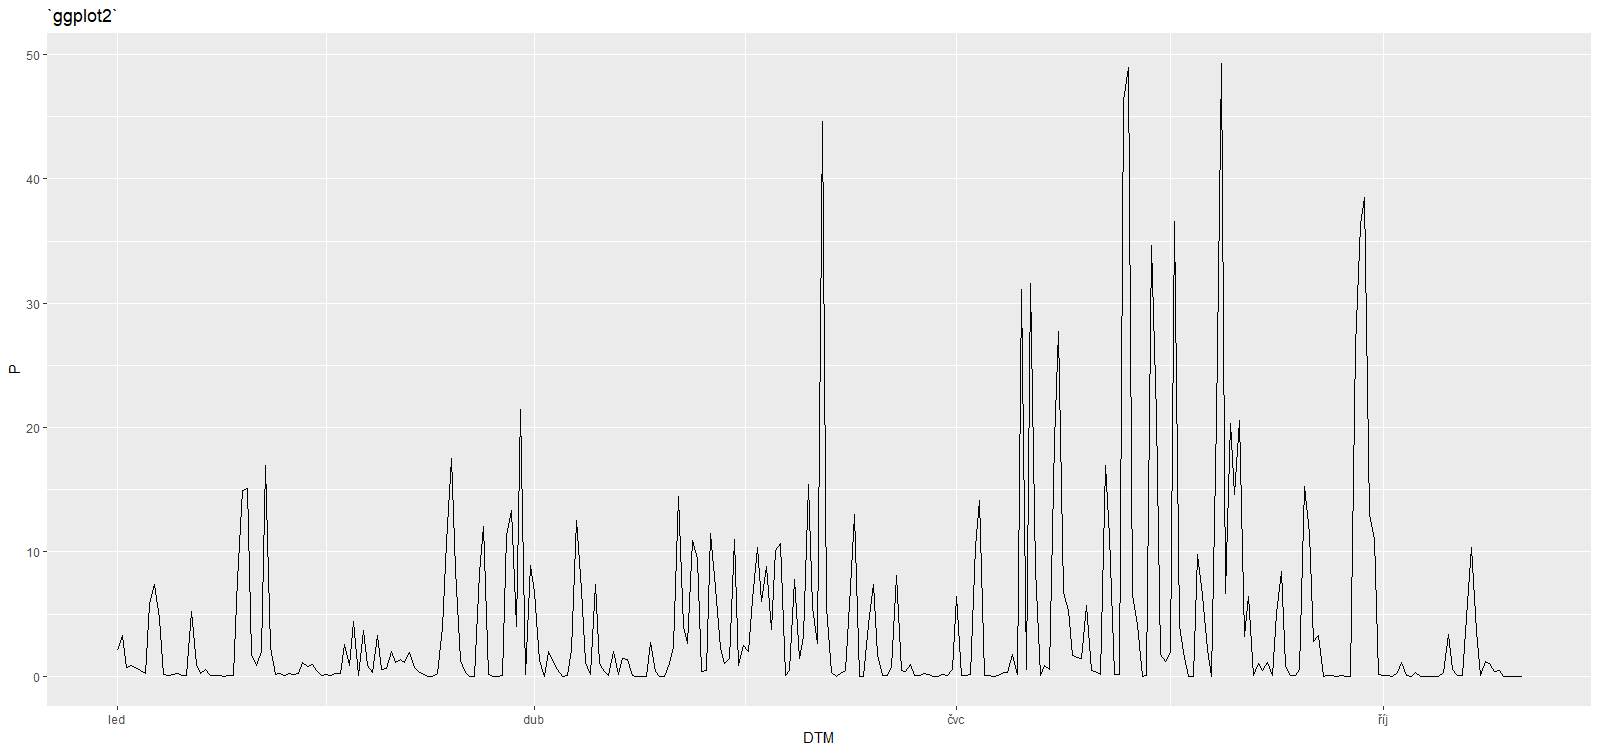
\includegraphics[width=\textwidth]{fig/3ggplot}
      \caption{Časová řada srážek na zvoleným povodí v roce 2010, \texttt{ggplot2}}
      \label{fig:ch4.1c}
\end{figure}

\subsubsection{4.2 Balíčky pro prostorovou
vizualizaci}\label{balicky-pro-prostorovou-vizualizaci}

\qquad V R existuje celá řada možností pro analýzu prostorových dat a
nástrojů k~jejich vykreslení. Důležitý rozdíl mezi R a tradičními
desktopovými GIS (\emph{geographical information system}) softwary je
ten, že GIS je primárně vytvořen k prostorové vizualizaci a zpracovává
data jedním přednastaveným způsobem, zatímco v R si uživatel sám musí
zvolit vhodné nástroje a odpovídající nastavení. Dále R neobsahuje
grafické uživatelské rozhraní (GUI), které by usnadňovalo práci s
prostorovými daty. Z tohoto důvodu může být R jako nástroj GIS pro nové
uživatele náročné. Hlavní výhodou R je, že přináší do tvorby prostorové
vizualizace silné výpočetní prostředky pro úpravu a statistickou analýzu
dat a možnost uložení skriptů a jejich další modifikace (Cheshire a
Lovelace 2015).

\qquad Prostorové objekty jsou často reprezentovány \emph{vektorovými}
daty. Takováto data obsahují popis \enquote{geometrie} nebo
\enquote{tvaru} území (body, linie a polygony) a většinou také obsahují
proměnné s dodatečnými informacemi o území (atributovou tabulkou). Dále
se také používají prostorová pole, která jsou obvykle reprezentována
pomocí \emph{rastrů}. Rastrová data se obvykle používají pro prostorově
kontinuální proměnné. Rastry dělí území mřížkou na buňky o stejné
velikosti neboli na \emph{pixely}, kterým je přiřazená hodnota dle
zájmové proměnné. Většinou se jedná o průměr či většinovou hodnotu pro
oblast spadající do konkretního pixelu. Na rozdíl od vektorových dat,
v~rastrových datech není informace o geometrii objektu uložená jako
souřadnice, ale v~rámci buněk. Velikost rastrových buněk neboli
prostorové rozlišení je dáno počtem řádků a sloupců, na které je území
rozdělené. (Hijmans {[}vid. 13.4.2018{]})

\begin{figure}[H]
  \centering
      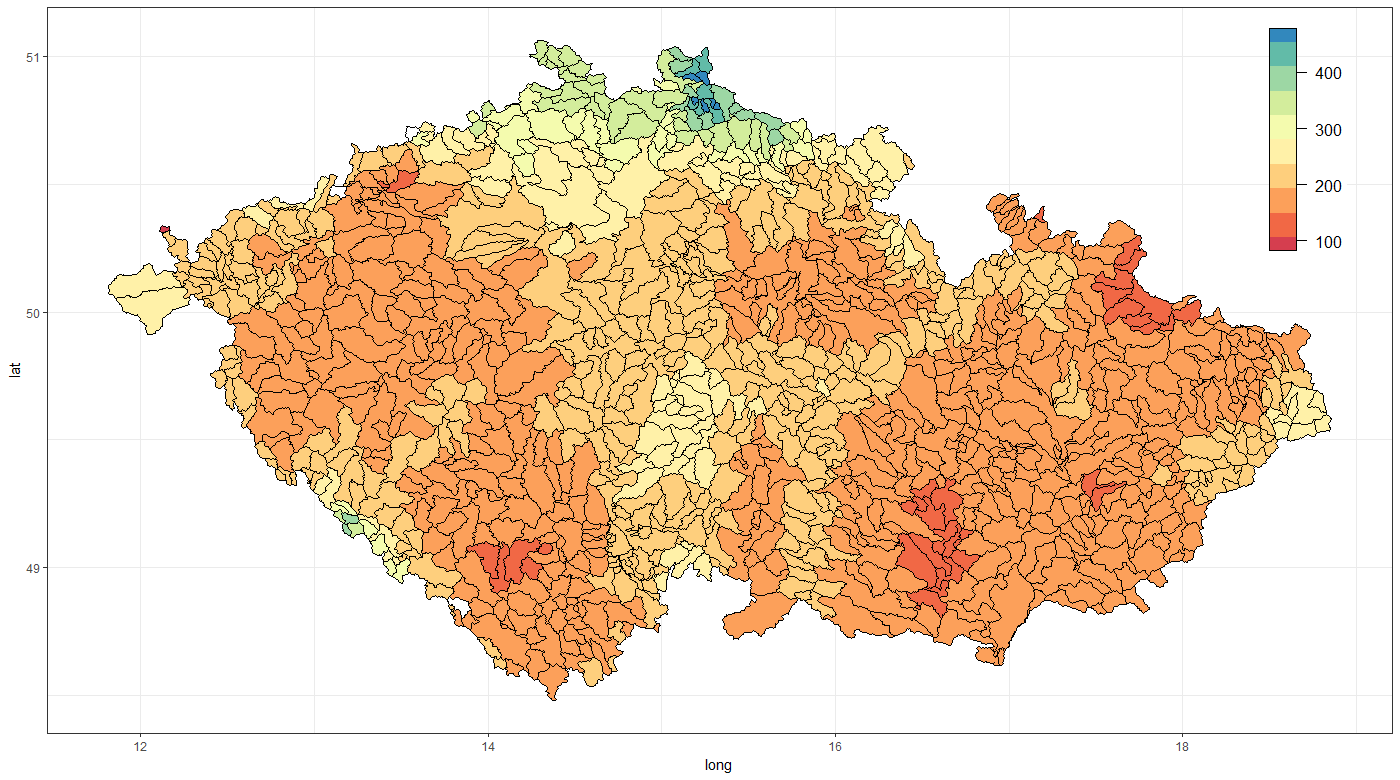
\includegraphics[width=\textwidth]{fig/ggplot_map2}
      \caption{Úhrn srážek (v mm) na povodích ČR za srpen 2010, vykresleno pomocí balíčků \texttt{ggplot2}}
      \label{fig:ch4.2}
\end{figure}

\qquad Vektorová data mohou být vykreslena v R pomocí celé řady balíčků
a to jak pomocí již zmíněných \texttt{base} (kapitola
\protect\hyperlink{baseviz}{4.1}) a \texttt{ggplot2} (kapitola
\protect\hyperlink{ggplot}{4.1.3}), tak i pomocí \texttt{Leaflet}
(kapitola \protect\hyperlink{leaflet}{4.3.3}). Příkladem vizualizace
vektorových dat pomocí balíčku \texttt{ggplot2} je vizualizace na
obrázku \ref{fig:ch4.2}.

\begin{figure}[H]
  \centering
      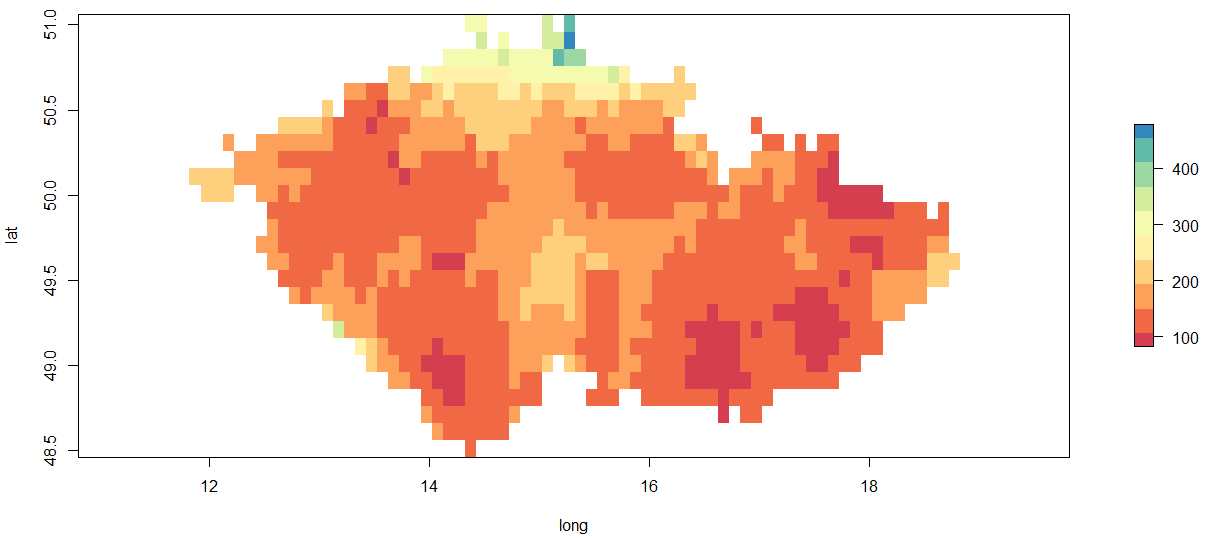
\includegraphics[width=\textwidth]{fig/raster_map2}
      \caption{Úhrn srážek (v mm) na povodích ČR za srpen 2010, vykresleno pomocí balíčků \texttt{raster}} 
      \label{fig:ch4.3}
\end{figure}

\qquad Balíček \texttt{raster} obsahuje funkce pro vytváření, čtení,
manipulaci, modelování, popis a analýzu rastrových dat. Podporuje práci
s velkými soubory a vytváření vlastních specifických funkcí (Hijmans
2017). Balíček \texttt{rasterVis} představuje metody pro vylepšenou
vizualizaci a interakci s rastrovými daty. Implementuje vizualizační
metody pro kvantitativní a kvalitativní data a to jak pro jednorozměrné,
tak i~vícerozměrné rastry. Dále poskytuje metody k zobrazení rastrů,
měnících se v čase, a~vektorových polí~(Lamigueiro 2018). Vykreslení dat
pomocí balíčku \texttt{raster} lze nalézt na obrázku \ref{fig:ch4.3}.

\hypertarget{htmlwidgets}{\subsubsection{4.3 Balíčky pro interaktivní
vizualizaci dat}\label{htmlwidgets}}

\qquad Možnost přiblížit, filtrovat či zobrazit podrobnosti grafu na
požádání je výhodou dynamických a interaktivních grafů. Interaktivní
grafy dokážou zobrazovat více informací a tím umožňují i hlubší
pochopení dat. Pro R existuje široká nabídka balíčků a nástrojů k
vytváření interaktivních grafů. Jednou z nejpopulárnějších\footnote{Dle
  žebříčku \href{https://www.rdocumentation.org/}{rdocumentation.org} je
  \texttt{htmlwidgets} 58. nejstahovanější balíček.} možností je balíček
\texttt{htmlwidgets}, jehož knihovna obsahuje užitečné nástroje pro
tvorbu téměř jakéhokoliv typu grafiky.

\qquad Balíček \texttt{htmlwidgets} poskytuje rozhraní pro snadné
propojení jazyka R a knihoven programovacího jazyka JavaScript,
používaného zejména pro webové aplikace. Tímto je umožněna bezproblémová
a konzistentní práce interaktivních map, grafů a~tabulek a to jak v
dokumentech \texttt{R\ Markdown} a v aplikacích \texttt{Shiny} (kapitola
\protect\hyperlink{shiny}{4.4.2}), tak i v rámci samotného R Studio.
\texttt{htmlwidgets} umožňuje vytváření vlastních \emph{widgets}, ale
především nabízí řadů již vytvořených, například \texttt{Plotly},
\texttt{Leaflet} a \texttt{dygraphs}. Tyto nástroje jsou dostupné
nejenom pro R, ale i pro další programovací jazyky (například Python)
(Vaidyanathan et al. 2018).

\hypertarget{plotly}{\paragraph{\texorpdfstring{4.3.1
\texttt{Plotly}}{4.3.1 Plotly}}\label{plotly}}

\qquad Balíček \texttt{Plotly} je vysokoúrovňové rozhraní pro open
source JavaScript vizualizační knihovnu \texttt{plotly.js}. Pro tvorbu
interaktivních vizualizací využívá jako základ balíček
\texttt{htmlwidgets}. Dále umožňuje jednoduchý převod \texttt{ggplot2}
grafů na interaktivní verzi. \texttt{Plotly} objekt lze vytvořit dvěma
způsoby, a to pomocí funkce \texttt{plot\_ly()}, která převádí data na
\texttt{Plotly} objekt, případně pomocí funkce \texttt{ggplotly()},
která převádí \texttt{ggplot2} objekt na \texttt{Plotly} objekt. Bez
ohledu na to, jak je \texttt{Plotly} objekt vytvořen, výsledkem je
interaktivní vizualizace, která ve své přednastavené verzi obsahuje
nástrojovou lištu a umožňuje přiblížení a pohyb po vizualizaci (Sievert
2018).

\hypertarget{dygraphs}{\paragraph{\texorpdfstring{4.3.2
\texttt{dygraphs}}{4.3.2 dygraphs}}\label{dygraphs}}

\qquad Balíček \texttt{dygraphs} je R rozhraním pro práci s
JavaScriptovou vizualizační knihovnou \texttt{dygraphs}. Poskytuje
bohaté možnosti k vykreslení časových řad v R, včetně podpory
interaktivních funkcí. Mezi tyto funkce patří například (RStudio {[}vid.
11.4.2018{]}):

\begin{itemize}
\tightlist
\item
  Automatické vykreslení časových řad typu \texttt{xts}\footnote{Objekt
    \texttt{xts} pochází z balíčku \texttt{xts}, který je rozšířením
    populárního balíčku pro práci s časovými řadami \texttt{zoo}.}
\item
  Vysoce konfigurovatelná nastavení os a vykreslení řad (včetně
  volitelné další osy~\(y\))
\item
  Zvýraznění, přiblížení řad či bodů
\item
  Zobrazení predikčních intervalů kolem řad
\item
  Umožňuje vykreslování překrývajících se grafů, vyznačení oblastí
  zastíněním a~označení určitých událostí svislými liniemi a popisky.
\end{itemize}

\vspace*{-0.4cm}

\hypertarget{leaflet}{\paragraph{\texorpdfstring{4.3.3
\texttt{Leaflet}}{4.3.3 Leaflet}}\label{leaflet}}

\qquad \texttt{Leaflet} je další z populárních open source JavaScript
vizualizačních knihoven pro interaktivní mapy. Využívají ji takové
webové stránky jako jsou
\href{http://www.nytimes.com/projects/elections/2013/nyc-primary/mayor/map.html}{\emph{The
New York Times}} a
\href{http://www.washingtonpost.com/sf/local/2013/11/09/washington-a-world-apart/?utm_term=.906188040dc1}{\emph{The
Washington Post}}, ale i
\href{https://blog.github.com/2013-06-13-there-s-a-map-for-that/}{\emph{GitHub}}
a \href{https://www.flickr.com/map}{\emph{Flickr}}. \texttt{Leaflet} je
také využíván GIS platformami jako jsou
\href{http://www.openstreetmap.org/\#map=7/49.714/15.060}{\emph{OpenStreetMap}},
\href{https://www.mapbox.com/}{\emph{Mapbox}} a
\href{https://carto.com/}{\emph{CartoDB}}.

\qquad Tento R balíček umožňuje integrování a ovládaní \texttt{Leaflet}
map. Mezi jeho funkce patří pohyb/přiblížení v rámci mapy, možnost
vytvářet mapy z libovolných kombinací (polygony, linie, markery, atd.).
Dále snadno vykresluje prostorové objekty z balíčků \texttt{sp} nebo
\texttt{sf} a datové soubory se sloupci zeměpisné šířky a délky.
\texttt{Leaflet} také poskytuje možnost ovládání interakcí v
\texttt{Shiny} aplikacích přes stávající hranice mapového výřezu či
reakce na kliknutí myši uživatelem. Umožňuje zobrazení map v~nesférickým
Mercatorově zobrazení a má mnoho dalších funkcí a doplňků (RStudio
{[}vid. 11.4.2018{]}). \vspace*{-0.2cm}

\hypertarget{webviz}{\subsubsection{4.4 Balíčky pro webové
aplikace}\label{webviz}}

\paragraph{\texorpdfstring{4.4.1
\texttt{flexdashboard}}{4.4.1 flexdashboard}}\label{flexdashboard}

\qquad \texttt{flexdashboard} slouží k publikaci dat a jejích přehledné
vizualizaci v rámci webového prohlížeče. Využívá \texttt{R\ Markdown} k
publikaci souvisejících vizualizací do jednotného zobrazení neboli
\emph{dashboard}u. Balíček podporuje široký výběr komponentů, včetně
\texttt{htmlwidgets}, \texttt{base}, \texttt{lattice} a \texttt{grid}
grafiky, tabulek, textových poznámek a~dalších. Vyznačuje se mimo jiné i
jednoduchým a flexibilním nastavením samotného rozvržení dashboardu a to
definováním řádků a sloupců. Komponenty takového dashboardu se pak
inteligentně přizpůsobí oknu prohlížeče, případně obrazovce mobilního
zařízení. Dále balíček umožňuje nastavení a přepínání mezi jednotlivými
záložkami dashboardu. Pro dynamické vizualizace lze kombinovat
\texttt{flexdashboard} a~\texttt{Shiny} aplikace. \vspace*{-0.2cm}

\hypertarget{shiny}{\paragraph{\texorpdfstring{4.4.2
\texttt{Shiny}}{4.4.2 Shiny}}\label{shiny}}

\qquad \texttt{Shiny} je balíček, umožňující jednoduché vytváření
interaktivních aplikací kombinací výpočetních možností R s
interaktivitou moderních webových stránek. Pomocí \texttt{Shiny} lze
vytvořit jak samostatnou aplikaci, běžící na webových stránkách, tak
i~lokální aplikaci bežící v prostředí R. Vzhled \texttt{Shiny} aplikace
lze modifikovat pomocí kaskádových stylů\footnote{Kaskádové styly (CSS)
  jazyk určený pro popis vzhledu elementů napsaných ve značkovacích
  jazycích (například HTML).}. (RStudio {[}vid. 14.4.2018{]})

\qquad Strukturou se \texttt{Shiny} aplikace liší od běžných skriptů.
Celá aplikace by měla být umístěna v jednom adresáři a celý skript by
měl být obsažen v souboru nazvaném \texttt{app.R}.\footnote{V dřívějších
  verzích \texttt{Shiny} bylo nutné skript rozdělit do dvou částí
  \texttt{ui} a \texttt{server}.} Aplikaci pak lze spustit pomocí
příkazu \texttt{runApp("cesta")}, kde \texttt{cesta} je cesta k adresáři
s aplikací. Skript \texttt{app.R} se skládá ze tří komponentů:

\begin{itemize}
\tightlist
\item
  Uživatelské rozhraní \texttt{ui}, které obsahuje rozložení ovládacích
  prvků a nastavení vzhledu.
\item
  \texttt{server} funkce, který obsahuje funkce generující samotné
  interaktivní výstupy.
\item
  \texttt{ShinyApp} funkce, která spojuje \texttt{ui} a server. \newline
\end{itemize}

\begin{Shaded}
\begin{Highlighting}[]
\KeywordTok{library}\NormalTok{(shiny)}

\NormalTok{ui <-}\StringTok{ }\KeywordTok{fluidPage}\NormalTok{()}

\NormalTok{server <-}\StringTok{ }\ControlFlowTok{function}\NormalTok{(input, output)\{\}}

\KeywordTok{shinyApp}\NormalTok{(}\DataTypeTok{ui =}\NormalTok{ ui, }\DataTypeTok{server =}\NormalTok{ server)}
\end{Highlighting}
\end{Shaded}

V rámci \texttt{ui} lze používat širokou řadu ovládacích prvků jako jsou
například tlačítka, zatrhávací políčka, přepínače, textové vstupy, atd.
Běžně se \texttt{ui} dělí do tří částí:

\begin{itemize}
\tightlist
\item
  Titulní panel, který obsahuje metadata, název aplikace a další
  relevantní informace.
\item
  Postranní panel, který nejčastěji obsahuje ovládací prvky.
\item
  Hlavní panel, který obsahuje výstupy generované funkcí
  \texttt{server}.
\end{itemize}

Příkladem ovládacího prvku vytvořeného v \texttt{ui} může být číselný
vstup, který umožňuje uživateli vložit libovolné číslo. Tento vstup je
označen pomocí \texttt{InputId} a v rámci \texttt{server} funkcí lze na
něj dle toho id odkázat. Konkretně tento vstup lze získat z~proměnné
\texttt{input\$num}. Obecně by to tedy mělo tvar
\texttt{input\$inputId}. Vstup z \texttt{ui} lze použit pouze v rámci
funkce \texttt{render*()}, případně v rámci funkce \texttt{reactive()}
(viz dále).

\begin{Shaded}
\begin{Highlighting}[]
\NormalTok{ui <-}\StringTok{ }\KeywordTok{fluidPage}\NormalTok{(}\KeywordTok{numericInput}\NormalTok{(}\DataTypeTok{inputId =} \StringTok{"num"}\NormalTok{,}
                             \DataTypeTok{label =} \StringTok{"Číselný vstup"}\NormalTok{,}
                             \DataTypeTok{value =} \DecValTok{10}\NormalTok{))}
\end{Highlighting}
\end{Shaded}

Funkce \texttt{server} přebírá vstupy z ovládacích prvků \texttt{ui} a
mapuje jednotlivé funkce k~výstupům. Příkladem takové funkce může být:

\begin{Shaded}
\begin{Highlighting}[]
\NormalTok{output}\OperatorTok{$}\NormalTok{histPlot <-}\StringTok{ }\KeywordTok{renderPlot}\NormalTok{(\{}
  \KeywordTok{hist}\NormalTok{(}\KeywordTok{rnorm}\NormalTok{(input}\OperatorTok{$}\NormalTok{num, }\DecValTok{1}\NormalTok{, }\DecValTok{0}\NormalTok{))}
\NormalTok{  \})}
\end{Highlighting}
\end{Shaded}

Tato funkce generuje grafický výstup v podobě histogramu normálního
rozdělení s~interaktivním počtem pozorování. Obecně pro generování
výstupu se používá funkce \texttt{render*()}. Tyto funkce mohou
obsahovat libovolný kód (například příprava dat, doprovodné výpočty,
atd.), ale je nutné, aby vraceli požadovaný typ výstupu. Základní
\texttt{render*()} funkce jsou vypsány v tabulce \ref{tab5}. Při změně
vstupu z \texttt{ui} v \texttt{render*()} dochází k přepočítání.

\begin{table}[H]
\centering
\begin{tabular}{|l|l|}
\hline
\multicolumn{1}{|c|}{funkce} & \multicolumn{1}{c|}{výstup} \\ \hline
\texttt{renderDataTable()}   & interaktivní tabulka        \\ \hline
\texttt{renderImage()}       & obrázek                     \\ \hline
\texttt{renderPlot()}        & graf                        \\ \hline
\texttt{renderPrint()}       & vytištěný blok kódu         \\ \hline
\texttt{renderTable()}       & tabulka                     \\ \hline
\texttt{renderText()}        & text                        \\ \hline
\texttt{renderUI()}          & \texttt{Shiny ui} element   \\ \hline
\end{tabular}
\caption{Základní \texttt{render*()} funkce}
\label{tab5}
\end{table}

\vspace*{-0.7cm}

\qquad Pro komplexní \texttt{Shiny} aplikaci s větším počtem
interaktivních prvků je vhodné použit funkce \texttt{reactive()} (tzv
reaktivní výrazy). Tato funkce slouží zejména jako prostředník mezi
\texttt{ui} a \texttt{render*()}. Na obrázku \ref{fig:ch4.4} je
znázorněn příklad struktury jednoduché \texttt{Shiny} aplikace s
použitím \texttt{reactive()} funkce. V tomto příkladu při změně
numerického vstupu (\texttt{input\$1}) se nejprve přepočítá
\texttt{reactive()} a následně \texttt{render*()\ A} a \texttt{B},
zatímco při změně vstupu \texttt{input\$2} či \texttt{input\$3} se
přepočítají pouze příslušné \texttt{render*()} výstupy \texttt{A} či
\texttt{B} se zachováním informací z \texttt{input\$1}.
\vspace*{-0.15cm}

\begin{figure}[H]
  \centering
      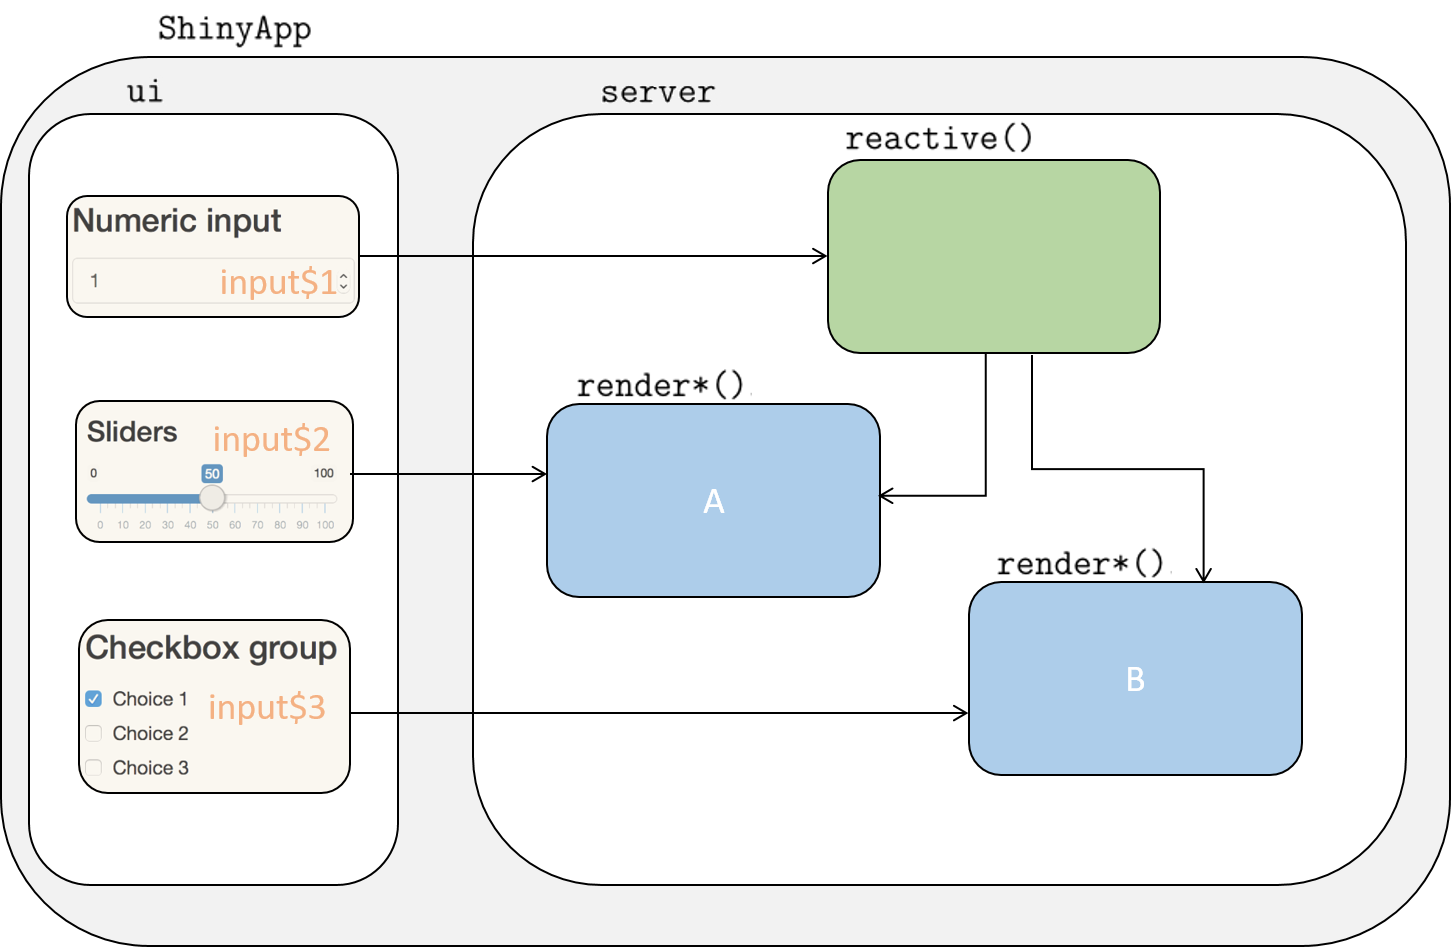
\includegraphics[width=0.7\textwidth]{fig/shiny}
      \caption{Ukázka \texttt{Shiny} aplikace s použitím funkce \texttt{reactive()}.} 
      \label{fig:ch4.4}
\end{figure}

\section*{Praktická část}\label{prakticka-cast}
\addcontentsline{toc}{section}{Praktická část}

\qquad Součástí práce je vytvoření webové aplikace pro vizualizaci a
analýzu hydrologické bilance a předpověď sucha v útvarech povrchových
vod ČR. Technické řešení aplikace je popsáno v části \enquote{Metodika},
jejíž součásti je i popis použitých dat a balíčků a postprocessingových
funkci. Dále následuje popis jednotlivých položek aplikace se zaměřením
na účel a funkčnost každé položky. Webová aplikace je výstupem řešení
projektu Činnosti k podpoře státní správy v problematice sucho v roce
2017 a 2018. Hlavním řešitelem je Výzkumný ústav vodohospodářský T. G.
Masaryka, v.v.i. Katedra vodního hospodářství a environmentálního
modelování (KVHEM) se na řešení projektu podílí subdodávkou tvořenou
zejména webovou aplikací \textbf{\emph{HAMR}}, kalibrací hydrologického
modelu Bilan a dalšími analýzami dat. Na řešení subdodávky se podílí
rozsáhlý tým KVHEM, v němž autorka této práce figuruje jako vývojářka
webové aplikace \textbf{\emph{HAMR}}.

\subsection{5 Metodika}\label{metodika}

\qquad Aplikace je vytvořena prostřednictvím programovacího jazyka R.
Jedná se o~vizualizaci výsledků modelování systému pro předpověď
hydrologické bilance \textbf{\emph{HAMR}}. Systém je založen na
propojení modelu vláhové bilance půdy \texttt{SoilClim}, modelu
hydrologické bilance \texttt{BILAN} a modelu vodohospodářské soustavy
\texttt{WATERES} jednotlivých povodí. Jádro aplikace je postaveno na
balíčcích \texttt{Shiny} a \texttt{flexdashboard}. Jak již bylo popsané
v kapitole \protect\hyperlink{webviz}{4.4}, \texttt{Shiny} umožňuje
jednoduché vytváření webových aplikací, interaktivních vizualizací v
prostředí R a balíček \texttt{flexdashboard} umožňuje pokročilé
formátovaní vzhledu. Společně slouží k publikaci dat a jejích přehledné
vizualizaci v~rámci webového prohlížeče.

\hypertarget{techres}{\subsubsection{5.1 Technické
řešení}\label{techres}}

\qquad Aplikace bude přístupná na
\href{https://shiny.fzp.czu.cz/KVHEM/HAMR/}{serveru fakulty}\footnote{Aplikace
  na serveru fakulty: \url{https://shiny.fzp.czu.cz/KVHEM/HAMR/}}, lze
ji také \href{https://github.com/KVHEM/Sucho}{stáhnout ze stránek
GitHubu}\footnote{Repozitář na GitHub:
  \url{https://github.com/KVHEM/Sucho}}, kde je pro aplikaci založen
repozitář. Tento repozitář obsahuje následující soubory:

\begin{itemize}
\tightlist
\item
  Soubor s aplikací \texttt{flex\_app.Rmd}
\item
  Skript připravující vstupní data pro aplikací \texttt{prep.R}
\item
  Skript pro automatickou instalaci potřebných balíčku
  \texttt{install.packages.R}
\item
  Soubor s kaskádovými styly pro nastavení vzhledu aplikace
  \texttt{styles.css}
\end{itemize}

Mimo již zmíněné balíčky \texttt{Shiny} a \texttt{flexdashboard} byly
použité následující balíčky:

\begin{itemize}
\tightlist
\item
  \texttt{leaflet}, umožňující vizualizaci prostorových dat v
  interaktivních mapách (kapitola \protect\hyperlink{leaflet}{4.3.3})
\item
  \texttt{ggplot2}, \texttt{dygraphs} a \texttt{Plotly} k vykreslení
  časových řad a čar překročení (kapitoly
  \protect\hyperlink{ggplot}{4.1.3}, \protect\hyperlink{dygraphs}{4.3.2}
  a \protect\hyperlink{plotly}{4.3.1})
\item
  \texttt{data.table}, \texttt{dplyr} sloužící k transformaci dat
\item
  \texttt{DT} je jedním z \emph{widgets} balíčku \texttt{htmlwidgets}
  (popsáno v kapitole \protect\hyperlink{htmlwidgets}{4.3}), sloužící k
  vytváření interaktivních tabulek.
\end{itemize}

Veškerý R kód použitý k vytvoření aplikace se nachází na datovém nosiči
jako příloha práce.

\hypertarget{data}{\subsubsection{5.2 Data}\label{data}}

\qquad Data, která využívá aplikace jsou velká, přibližně 1.17 GB, a
jsou chráněna licencí. Většinou se totiž jedná o majetek ČHMU a VÚV
T.M.G. Z těchto důvodů data jsou zatím uložena zvlášť na
OwnCloud\footnote{OwnCloud je open source cloudová služba, více o této
  službě zde: \url{https://owncloud.org/features/}} úložišti, ke kterému
mají přístup pouze řešitelé projektu. Pro offline chod aplikace je tedy
nezbytné, mít přístup na toto úložiště. Pro účely této bakalářské práce
se veškerá potřebná data nachází na datovém nosiči jako příloha práce.
Verze publikovaná na serveru KVHEM pochopitelně využívá vlastní kopii
dat.

\begin{figure}[H]
      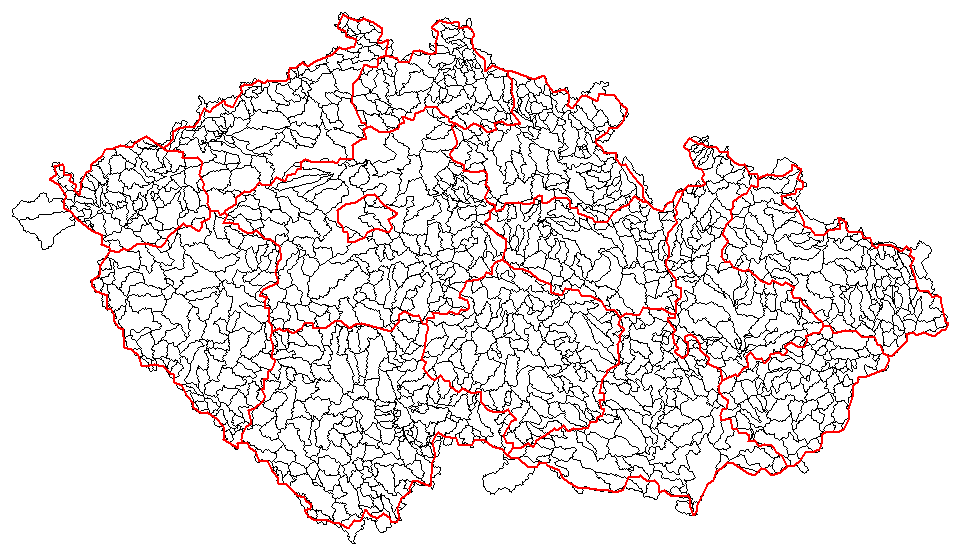
\includegraphics[width=\textwidth]{fig/povodi-kraje}
      \caption{Útvary povrchových vod (UPOV) (vyznačené černě) a kraje (vyznačené červeně) ČR}
      \label{fig:ch5.0}
\end{figure}

\begin{figure}[H]
      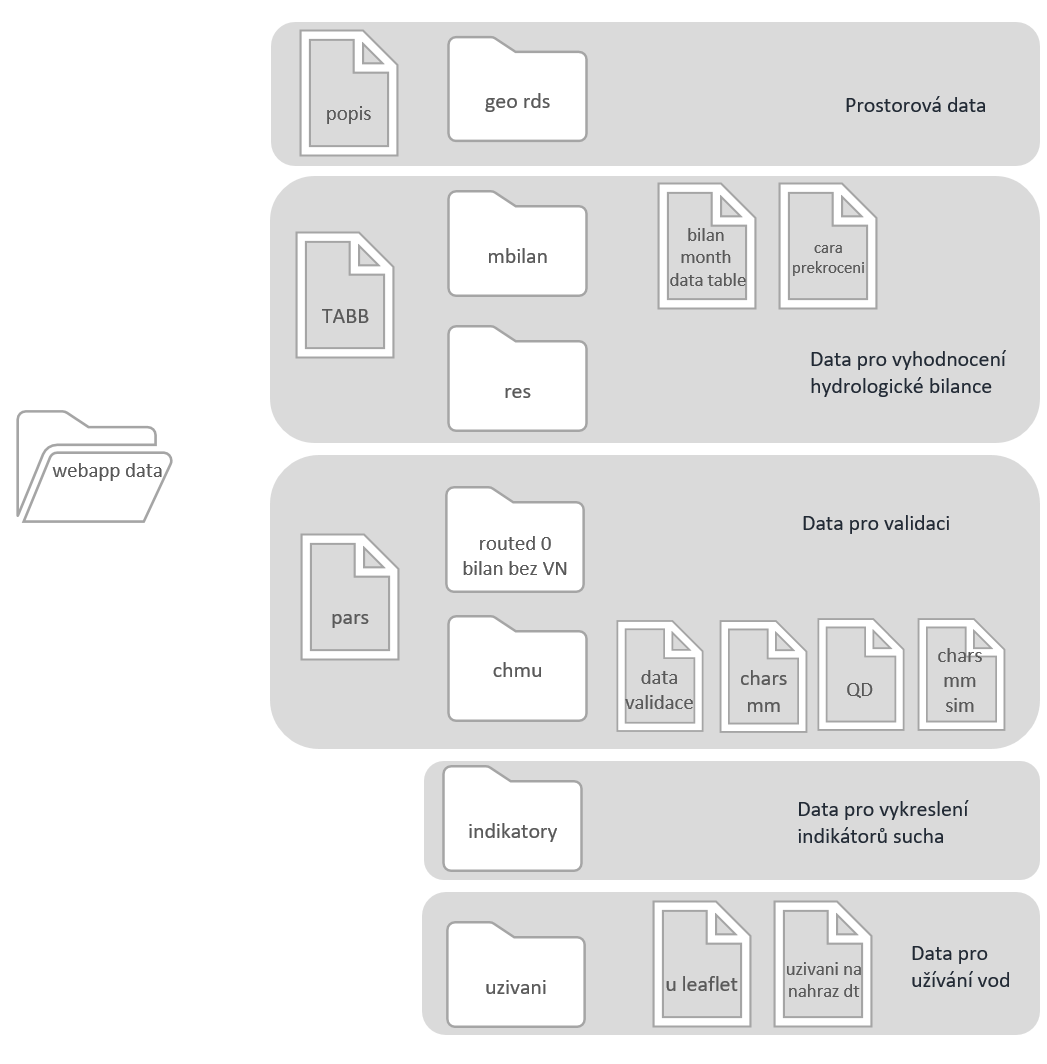
\includegraphics[width=\textwidth]{fig/struktura2}
      \caption{Struktura složek aplikace}
      \label{fig:ch5.1}
\end{figure}

\qquad Vizualizovaná data lze rozdělit do několika skupin: prostorová
data, data potřebná pro hydrologickou bilanci, data pro indikátory
sucha, data pro užívání vod a data pro validaci. Skupina prostorových
dat obsahuje soubory s informacemi o útvarech povrchových vod (UPOV) ČR
(\texttt{povodi.rds}, \texttt{reky.rds}, \texttt{jezera.rds},
\texttt{nadrze.rds}) a soubory administrativního členění ČR
(\texttt{kraje.rds}, \texttt{okresy.rds} a povodí 3. řadu
\texttt{povodi\_III.rds}) viz obrázek \ref{fig:ch5.0}. Přesná struktura
složek aplikace je vyobrazená na diagramu \ref{fig:ch5.1}. Tyto soubory
byly v rámci přípravy dat převedeny z formátu .shp do formátu .rds. Dále
pro rychlejší načítání a jednodušší manipulaci byly tyto soubory
transformovány do souřadnicového systému WGS84 (pomocí funkce
\texttt{spTransform()} z~balíčku \texttt{sp} a atributu \texttt{CRS} -
\emph{Coordinate Reference System} - nastaveného na identifikátor pro
WGS84 - EPSG:4326) a zjednodušeny (pomocí funkce \texttt{ms\_simplify()}
z balíčku \texttt{rmapshaper}) pro snížení náročnosti při vykreslování.
Soubor \texttt{popis.rds} obsahuje informace o jednotlivých útvarech
jako jsou název útvaru, název povodí, název oblasti, kategorie útvaru a
typ útvaru. Následně soubor \texttt{popis.rds} je propojen pomocí funkce
\texttt{merge()} z balíčku \texttt{sp} se souborem \texttt{povodi.rds}
přes identy jednotlivých útvaru (\texttt{UPOV\_ID}). K vykreslení
horního povodí se používá soubor \texttt{TABB.rds} obsahující informace
o tom, která povodí přitékají do jednotlivých UPOVů.

\qquad Další skupinou jsou data potřebná pro vyhodnocení hydrologické
bilance. Pomocí modelu Bilan (Vizina et al. 2015) bylo v rámci projektu
kalibrováno 1112 UPOVů a~výstupem je 18 proměnných (složky hydrologické
bilance a meteorologické vstupy) pro každý UPOV v denním kroku pro
období \mbox{1981-2010}. Tyto proměnné jsou uvedeny v tabulce \ref{tab6}
(VÚV TGM 2015). Z důvodů šetření vnitřní paměti aplikace se soubory
s~daty pro hydrologickou bilanci nacházejí na úložišti ve složce
\enquote{res} a jsou uloženy ve formátu .rds s názvy odpovídající
identům jednotlivých povrchových útvarů (\texttt{UPOV\_ID}). Aplikace
tyto soubory načítá pouze při požadavku uživatele. Měsíční bilance je
agregací denních dat a načítá se ze souboru
\texttt{bilan\_month\_data\_table.rds} (ukládá se do proměnné
\texttt{BM}). Do teto skupiny lze zařadit i soubor
\texttt{cara\_prekroceni\_dt.rds} (v~aplikaci proměnná \texttt{cp}).
Soubor obsahuje předpočítané roční, měsíční a sezónní pravděpodobnosti
spočítané přes jednotlivé proměnné dle vzorce
\mbox{$p = (m-0.3)/(n+0.4)$}, kde po seřazení souboru dle velikosti v
klesajícím pořadí je \(n\) počet prvků a \(m\) je pořadové číslo.

\begin{table}[H]
\centering
\begin{tabular}{|c|c|c|c|}
\hline
zkratka      & význam                       & zkratka       & význam                                                                                   \\ \hline
\texttt{P}   & srážky na povodí             & \texttt{SW}   & \begin{tabular}[c]{@{}c@{}}půdní vlhkost (zásoba \\ vody v nenasycené zóně)\end{tabular} \\ \hline
\texttt{R}   & odtok (pozorovaný)           & \texttt{SS}   & zásoba vody ve sněhu                                                                     \\ \hline
\texttt{RM}  & celkový odtok (simulovaný)   & \texttt{GS}   & zásoba podzemní vody                                                                     \\ \hline
\texttt{BF}  & základní odtok (simulovaný)  & \texttt{INF}  & infiltrace do půdy                                                                       \\ \hline
\texttt{B}   & základní odtok (odvozený)    & \texttt{PERC} & perkolace z půdní vrstvy                                                                 \\ \hline
\texttt{DS}  & zásoba pro přímý odtok       & \texttt{RC}   & dotace zásoby podzemní vody                                                              \\ \hline
\texttt{DR}  & přímý odtok                  & \texttt{T}    & teplota vzduchu                                                                          \\ \hline
\texttt{PET} & potenciální evapotranspirace & \texttt{H}    & vlhkost vzduchu                                                                          \\ \hline
\texttt{ET}  & územní výpar                 & \texttt{WEI}  & váhy pro kalibraci odtoku                                                                \\ \hline
\end{tabular}
\caption{Výstupy kalibrace denního modelu Bilan}
\label{tab6}
\end{table}

\qquad Data pro vykreslení indikátorů sucha se nacházejí ve samostatné
složce \enquote{indikatory}. Při zvolení uživatelem indikátoru sucha (v
nabídce momentálně jsou pouze indikátory SPI a SPEI spočítány klouzavě s
krokem 1, 3, 6, 9 a 12 měsíců) se načte .rds soubor dle odpovídajícího
indikátoru a kroku.

\qquad Data užívání vod za období 2006-2016
(\texttt{uzivani\_na\_nahraz\_dt.rds} ve složce \enquote{uzivani})
pocházejí z evidence užívání vod, kterou spravuje VÚV T. G. Masaryka a v
rámci aplikace se ukládají do proměnné \texttt{u}. Data obsahují
informace o poloze odběru ve formě souřadnic (\texttt{X} a \texttt{Y}),
identifikačním čísle odběru (\texttt{ICOC}), názvu místa odběru
(\texttt{NAZICO}) a také informace o jevu (odběry z podzemních vod
\texttt{POD}, odběry z povrchových vod \texttt{POV} či vypouštění
\texttt{VYP}). V rámci přípravy dat byly \texttt{ICOC}ům, které
obsahovali pozorované údaje, ale měli chybějící souřadnice, přiřazeny
průměry souřadnic mezi odběry se stejným \texttt{ICOC} a jiným jevem.
Tyto data slouží k vykreslení časových řad a tabulek. Pro vykreslení
bodů do mapy bylo nutné vytvořit soubor (\texttt{u\_leaflet.rds} ve
stejné složce), který obsahuje pouze jeden záznam pro každý
\texttt{ICOC}. Souřadnice těchto \texttt{ICOC}ů byly transformovány do
souřadnicového systému WGS84 a~následně byly uloženy ve formátu
\texttt{SpatialPointsDataFrame}.

\qquad Kalibrace modelu Bilan proběhla s nastavením modelu na denní
časový krok při použití šesti volných parametrů (\emph{Spa}, \emph{Alf},
\emph{Dgm}, \emph{Soc}, \emph{Mec}, \emph{Grd}). Parametry jsou popsány
v tabulce \ref{tab7} (VÚV TGM 2015). Soubor s parametry
\texttt{pars.rds} se nahrává v aplikaci do stejnojmenné proměnné a
obsahuje počáteční hodnoty parametrů (\texttt{initial}), jejích dolní a
horní meze (\texttt{lower}, \texttt{upper}) a stávající hodnotu
(\texttt{current}). Tyto proměnné jsou dány pro každý UPOV. K stanovení
hodnot parametrů byl použit globální optimalizační algoritmus
diferenciální evoluce (VÚV TGM 2015).

\begin{table}[H]
\centering
\begin{tabular}{|c|l|l|l|}
\hline
název  & \multicolumn{1}{c|}{\texttt{Alf}}                                                                                                                  & \multicolumn{1}{c|}{\texttt{Dgm}}                                                                                                                                                  & \multicolumn{1}{c|}{\texttt{Grd}}                                                             \\ \hline
význam & \begin{tabular}[c]{@{}l@{}}parametr určující \\ odtok ze zásoby \\ pro přímý odtok\end{tabular}                                                    & \begin{tabular}[c]{@{}l@{}}koeficient mezi teplotou\\  a táním sněhu\end{tabular}                                                                                                  & \begin{tabular}[c]{@{}l@{}}parametr určující \\ odtok ze zásoby \\ podzemní vody\end{tabular} \\ \hline
název  & \multicolumn{1}{c|}{\texttt{Mec}}                                                                                                                  & \multicolumn{1}{c|}{\texttt{Soc}}                                                                                                                                                  & \multicolumn{1}{c|}{\texttt{Spa}}                                                             \\ \hline
význam & \begin{tabular}[c]{@{}l@{}}parametr rozdělující\\ perkolaci na přímý \\ odtok a na dotaci \\ podzemní vody pro \\ podmínky tání sněhu\end{tabular} & \begin{tabular}[c]{@{}l@{}}koeficient mezi teplotou \\ a táním parametr \\ rozdělující perkolaci na \\ přímý odtok a na dotaci \\ podzemní vody pro letní \\ podmínky\end{tabular} & \begin{tabular}[c]{@{}l@{}}kapacita zásoby\\  půdní vlhkosti\end{tabular}                     \\ \hline
\end{tabular}
\caption{Parametry denního modelu Bilan}
\label{tab7}
\end{table}

\qquad Model byl kalibrován na hydrologické charakteristiky povodí UPOV
(m-denní průtoky a dlouhodobý průměrný průtok) poskytnuté ČHMÚ. M-denní
průtoky vypočítané na základě pozorovaných hodnot lze načíst ze souboru
\texttt{chars\_mm.rds} a~m-denní průtoky pro simulována data ze souboru
\texttt{chars\_mm\_sim.rds}.

\qquad K validaci denních průtoků (soubor \texttt{QD.rds} ze složky
\enquote{chmu}) bylo využito dat ze 156 vodoměrných stanic. Po propojení
databankového čísla \texttt{DBCN} s povodím \texttt{UPOV\_ID} zbylo 153
stanic. Mimo \texttt{DBCN} a \texttt{UPOV\_ID} soubor obsahuje hodnoty
pozorovaných denních průtoků (\texttt{value}) za období 1980-2010
(\texttt{DTM}). Simulované průtoky se nacházejí ve složce
\enquote{routed-0\_bilan\_bez\_VN} a obdobně jako u denních dat
hydrologické bilance obdrží se při zvolení konkrétní stanice (dle
patřičného \texttt{UPOV\_ID} aplikace načte odpovídající .rds soubor).
Pro prostorové vykreslení stanic se používá soubor \texttt{QD\_stanice}
(složka \enquote{geo\_rds}, soubor \texttt{stanice.rds}). Původní
shapefile byl převeden do souřadnicového systému WGS84 a uložen ve
formátu .rds. Soubor obsahuje nejen prostorové informace, ale i
informace o názvech toku, ploše povodí atd.

\qquad Validace měsíčních průtoků využívá záznamy 542 vodoměrných stanic
z~období 1982-2010. Prostorová data jsou uložená do proměnné
\texttt{stanice} (soubor \texttt{E04\_Vodomerne\_stanice.rds} ze složky
\enquote{geo\_rds}). Data s naměřenými (\texttt{QMER}) a simulovanými
(\texttt{QNEX}, \texttt{QNEY}) průtoky lze načíst ze souboru
\texttt{data\_validace.rds} ze složky \enquote{chmu}. Tento soubor byl
vytvořen agregací denních dat ze složky
\enquote{routed-0\_bilan\_bez\_VN}.

\subsubsection{5.3 Postprocessing}\label{postprocessing}

\qquad Pro podporu projektu byl vytvořen balíček
\texttt{CatCa}\footnote{Repozitář na GitHub:
  \url{https://github.com/KVHEM/CatCa}.}, který obsahuje některé
důležité funkce pro práci s útvary povrchových vod, výpočet bilance,
m-denních vod atd. Nainstalovat balíček lze pomocí příkazu
\texttt{devtools::install\_github("KVHEM/CatCa")}. V rámci tvorby
aplikace byly do tohoto balíčků přidány také funkce pro přípravu dat.
Tyto funkce upravují vstupní data do potřebného formátu a vybírají pouze
potřebné proměnné pro snížení využívané paměti a výpočetní náročností.
Přehled funkcí k přípravě dat je v tabulce~\ref{tab8}. Dále balíček
obsahuje funkci \texttt{give\_paths()} pro nastavení pracovních cest k
úložišti dat. Pokud cesta není nastavena pomocí funkce
\texttt{give\_paths()} je nutné jí uložit manuálně do proměnné
\texttt{.datadir}.

\begin{table}[H]
\centering
\begin{tabular}{|l|l|}
\hline
\texttt{prep\_spatial\_data()}   & příprava prostorových dat pro aplikaci                     \\ \hline
\texttt{prep\_bilan\_month()}    & příprava měsíční bilance pro aplikaci                      \\ \hline
\texttt{prep\_QD()}             & příprava denních průtoku (validace) pro aplikaci  \\ \hline
\texttt{prep\_uzivani()}        & příprava užívaní pro aplikaci                              \\ \hline
\texttt{prep\_uzivani\_upovid()} & příprava připojeni \texttt{UPOV\_ID} k užívaní pro aplikaci \\ \hline
\end{tabular}
\caption{Přehled funkcí z balíčku \texttt{CatCa} pro přípravu dat}
\label{tab8}
\end{table}

\subsection{6 Základní rozvržení}\label{zakladni-rozvrzeni}

\qquad Na úvod je vhodné uvést některé pojmy, které budou používány pro
popis základního rozvržení aplikace. Okno aplikace je většinou rozděleno
do několika hlavních části: boční panel, panel s mapovým výstupem a
panel s grafickými výstupy. V bočním panelu se nastavují vstupy pro
vykreslení mapy, požadované vrstvy a lze také použit pole pro
vyhledávaní útvaru. Pole \enquote{Vyhledávaní útvaru} nabízí seznam
všech vykreslených útvarů, ale lze ho také použít k ručnímu vyhledávání;
stačí vymazat momentálně zobrazený název a napsat název toku či jeho
\texttt{UPOV\_ID}. Pole \enquote{Vrstvy} v bočním panelu je k dispozici
pro každý panel s mapovým výstupem aplikace a~umožňuje výběr
následujících vrstev: povodí, řeky, jezera, nádrží, mapový podklad,
povodí 3. řádu a administrativní členění České republiky (kraje a
okresy). Boční panel některých záložek také obsahuje tlačítka
\enquote{Reset} a \enquote{Zobrazit}. Tlačítko \enquote{Reset} vrací
mapový panel na počátečně nastavené souřadnice. Tlačítko
\enquote{Zobrazit} slouží k~vykreslení po novém nastavení vstupů. Horní
lišta aplikace obsahuje přepínač mezi jednotlivými záložkami aplikace:
\enquote{Základní mapa}, \enquote{Indikátory sucha}, \enquote{Užívání},
\enquote{Validace} a \enquote{O projektu}. Záložka \enquote{O projektu}
obsahuje krátký popis projektu a~veškeré kontakty. V budoucnu bude
rozšířena o metodiky k jednotlivým součástem systému.

\begin{figure}[H]
      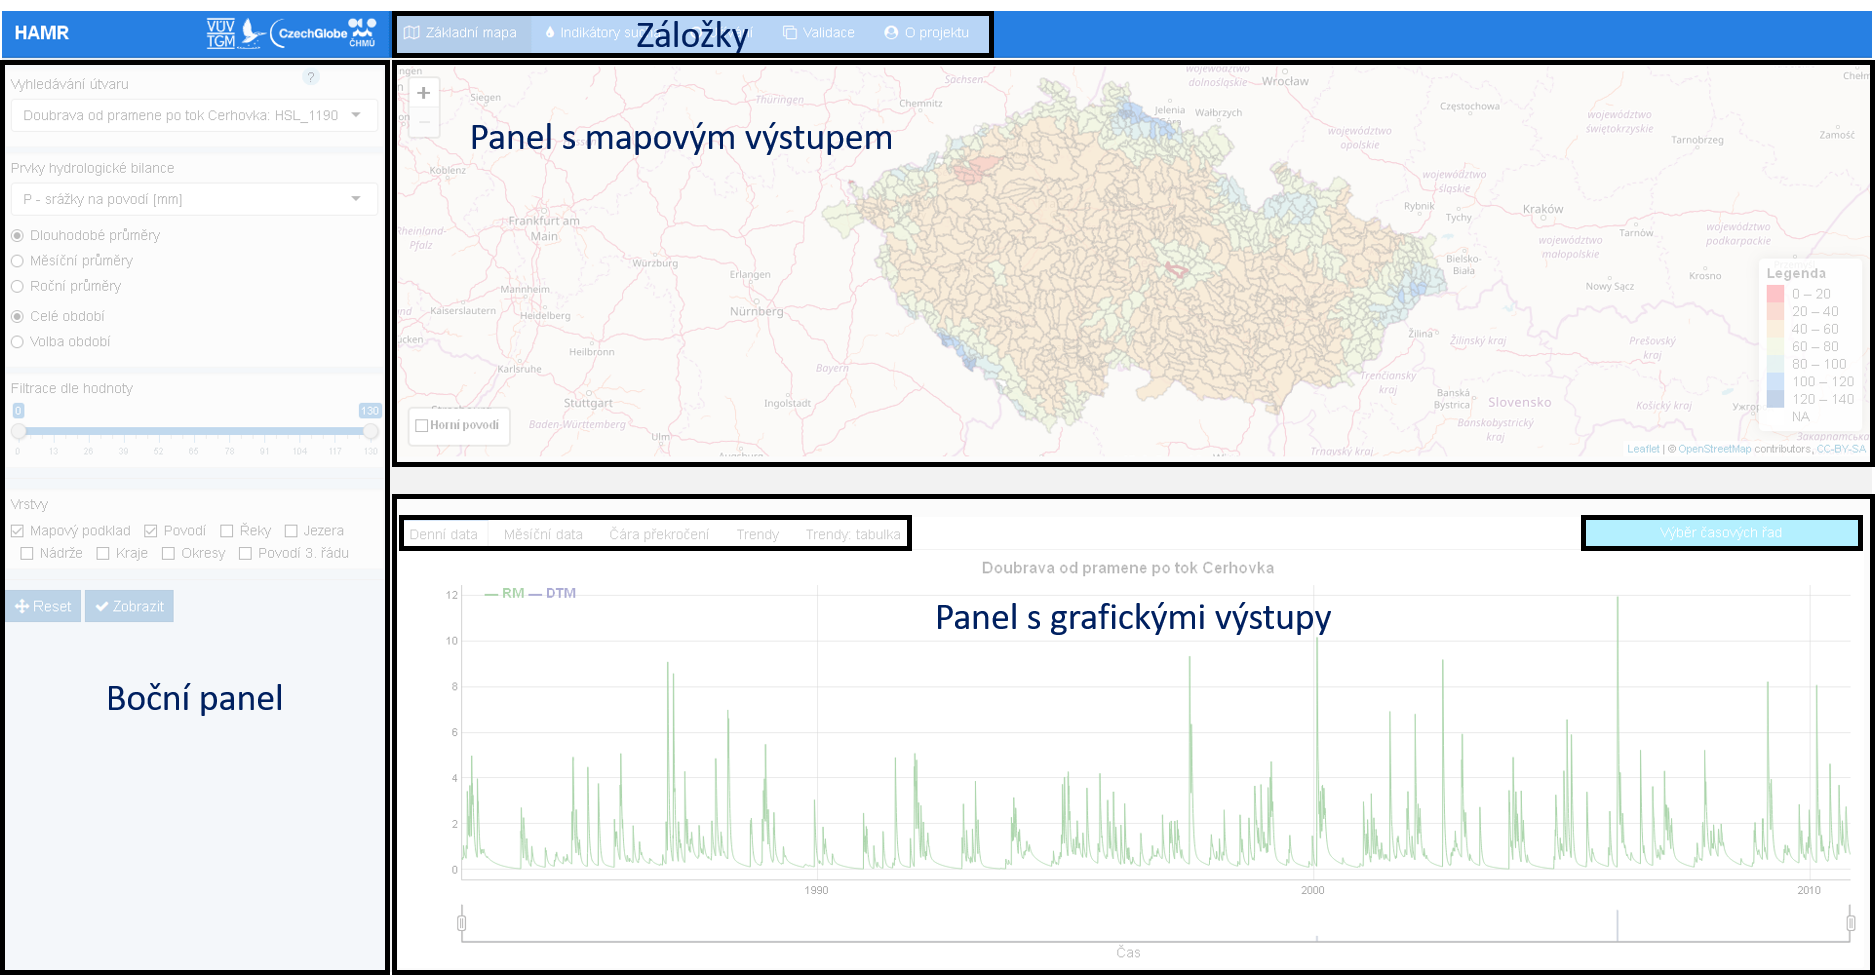
\includegraphics[width=\textwidth]{fig/rozlozeni2}
      \caption{Základní rozloženi okna aplikace}
      \label{fig:ch5.2}
\end{figure}

\qquad Grafy zpravidla mají vlastní výběr proměnných, který se na
obrázku \ref{fig:ch5.2} nachází v pravém horním rohu grafického panelu.
Tento výběr má tvar srolovatelného menu. Dále grafický panel může
obsahovat vlastní lištu se záložkami pro přepínání mezi jednotlivými
typy grafů a tabulek.

\subsubsection{6.1 Základní mapa}\label{zakladni-mapa}

\qquad \enquote{Základní mapa} (obrázek \ref{fig:ch5.3}) je první
záložkou a zobrazí se ihned po spuštění aplikace. Obsahuje informace o
hydrologické bilanci povodí České republiky. Záložka základní mapa je
rozložena na boční panel, panel s mapovým výstupem a panel s~grafickým
výstupem.

\qquad V bočním panelu se nacházejí pole \enquote{Vyhledávání útvaru},
\enquote{Prvky hydrologické bilance}, \enquote{Filtrace dle hodnoty},
\enquote{Vrstvy} a tlačítka \enquote{Reset} a \enquote{Zobrazit}.
Uživatel volí proměnnou hydrologické bilance, dle níž budou zbarveny
jednotlivá povodí zobrazená na mapě. Hodnoty proměnné jsou agregovány do
měsíčních a ročních kroků, lze je také vykreslit jako dlouhodobé
průměry, tzn. průměry za celé období nebo za konkrétní periody po 29
letech: 1961-1990, 1971-2000 a 1981-2010. \enquote{Filtrace dle hodnoty}
v počátečním stavu obsahuje všechny hodnoty zvolené proměnné a dále
umožňuje nastavení rozsahu hodnot, který omezí vykreslená povodí.
\enquote{Vyhledávání útvaru} je jedinou částí bočního panelu, která je
propojená nejenom s mapou, ale i s grafickými výstupy, a to pomocí
funkce \texttt{renderUI()} z balíčků \texttt{Shiny} (kapitola
\protect\hyperlink{shiny}{4.4.2}), která umožňuje, aby element
uživatelského rozhraní \texttt{ui} obsahoval vstup
\texttt{input\$map\_shape\_click\$id}. Tento vstup je získán po kliknutí
na mapový objekt, vytvořený pomocí \texttt{Leaflet} (kapitola
\protect\hyperlink{leaflet}{4.3.3}) a vrací \texttt{UPOV\_ID} příslušný
tomuto mapovému objektu. Objekt \texttt{search.choices} obsahuje seznam
všech \texttt{UPOV\_ID} s přiřazenými názvy toků.

\begin{figure}[H]
      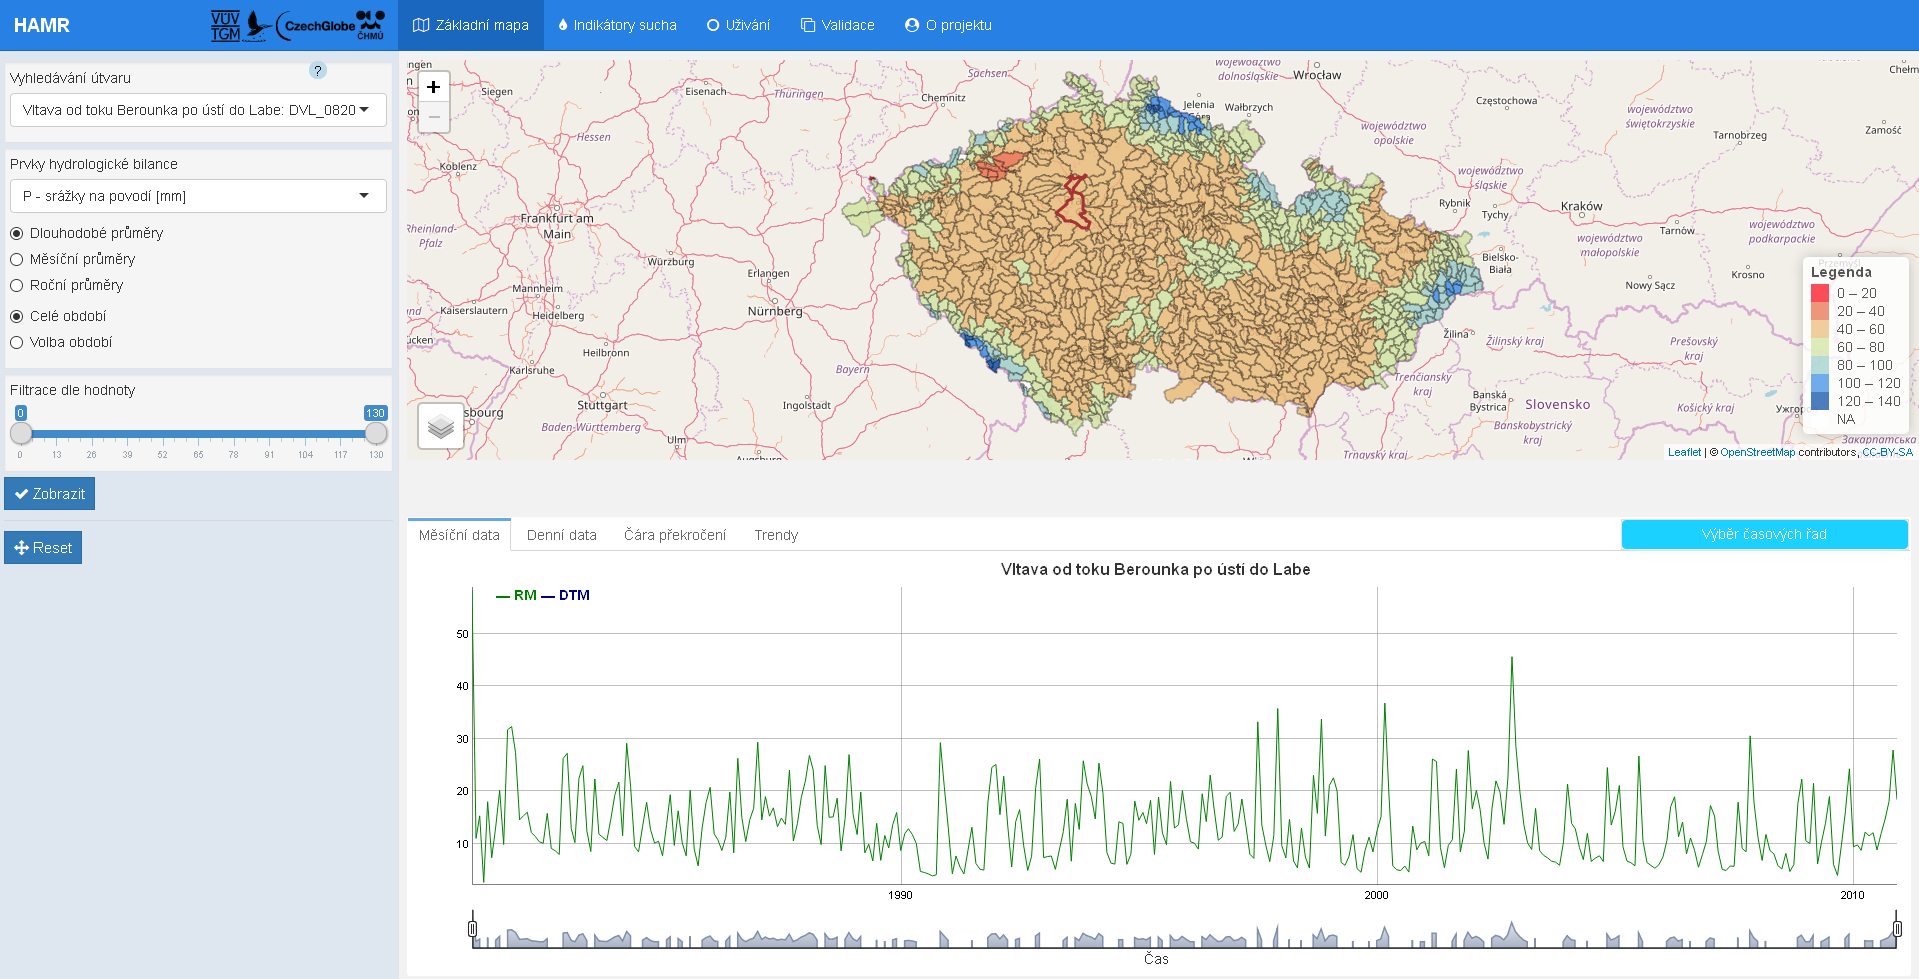
\includegraphics[width=\textwidth]{fig/P_ZM}
      \caption{Záložka aplikace "Základní mapa"}
      \label{fig:ch5.3}
\end{figure}

\begin{Shaded}
\begin{Highlighting}[]
\KeywordTok{renderUI}\NormalTok{(\{}\KeywordTok{selectizeInput}\NormalTok{(}\DataTypeTok{inputId =} \StringTok{"search.id"}\NormalTok{, }
                         \DataTypeTok{label =} \StringTok{"Vyhledávání útvaru"}\NormalTok{,}
                         \DataTypeTok{selected =}\NormalTok{ input}\OperatorTok{$}\NormalTok{map_shape_click}\OperatorTok{$}\NormalTok{id,}
                         \DataTypeTok{choices =}\NormalTok{ search.choices)\})}
\end{Highlighting}
\end{Shaded}

\qquad Mapové objekty jsou vykresleny pomocí \texttt{Leaflet}. V rámci
objektu \texttt{leaflet()} lze použit tyto funkce k nastavení:
\texttt{setView()} nastaví počáteční souřadnice a přiblížení,
\texttt{addTiles()} vykreslí mapový podklad. Aplikace používá
přednastavený podklad OpenStreetMap (RStudio {[}vid. 11.4.2018{]}).
Objekty jsou vykresleny pomocí funkce \texttt{add*()}, která v názvu
obsahuje typ objektu, například \texttt{addPolylines()},
\texttt{addPolygons()} atd. Struktura objektu \texttt{leaflet()} pak
může vypadat například následovně

\begin{Shaded}
\begin{Highlighting}[]
\NormalTok{map <-}\StringTok{ }\KeywordTok{leaflet}\NormalTok{() }\OperatorTok
\StringTok{          }\KeywordTok{setView}\NormalTok{(...) }\OperatorTok\StringTok{ }
\StringTok{          }\KeywordTok{addTiles}\NormalTok{(...) }\OperatorTok\StringTok{ }
\StringTok{          }\KeywordTok{addPolygons}\NormalTok{(...)}
\end{Highlighting}
\end{Shaded}

\qquad Při změně vstupu v bočním panelu je nutné znovu překreslit mapový
objekt. Tento přístup může být pro jiné interaktivní funkce příliš
výpočetně náročný. Například vrstva \enquote{Horní povodí}, která
zobrazuje povodí přitékající do momentálně vybraného povodí, je z toho
důvodu vykreslována pomocí \texttt{leafletProxy()}. Tento příkaz
umožňuje okamžité změny, na již vykresleném mapovém objektu. Konkrétně
kód pro aktualizaci horního povodí je uveden níže.

\begin{Shaded}
\begin{Highlighting}[]
\KeywordTok{observe}\NormalTok{(\{}
  \KeywordTok{leafletProxy}\NormalTok{(}\StringTok{"map"}\NormalTok{) }\OperatorTok
\StringTok{    }\KeywordTok{clearGroup}\NormalTok{(}\StringTok{"Horní povodí"}\NormalTok{) }\OperatorTok
\StringTok{    }\KeywordTok{addPolylines}\NormalTok{(}\DataTypeTok{data=}\KeywordTok{horni.povodi}\NormalTok{(),}
                 \DataTypeTok{color =} \StringTok{"#00264d"}\NormalTok{, }\DataTypeTok{weight =} \FloatTok{2.5}\NormalTok{, }
                 \DataTypeTok{opacity =} \FloatTok{0.7}\NormalTok{, }\DataTypeTok{stroke =} \OtherTok{TRUE}\NormalTok{,}
                 \DataTypeTok{group =} \StringTok{"Horní povodí"}\NormalTok{) }
\NormalTok{\})}
\end{Highlighting}
\end{Shaded}

\qquad Pro zvolené povodí se vypočítají časové řady z měsíčních a
denních dat (pomocí balíčku \texttt{dygraphs}), čára překročení pro celé
období, roční období a měsíce (pomocí balíčku \texttt{Plotly}) a trendy:
grafické znázornění a tabulka s vyhodnocením statistické významnosti
(\texttt{ggplot2}). Zvolené povodí se zvýrazní v mapě červeným okrajem
pomocí \texttt{leafletProxy()}. Kliknutím na jiné povodí se přepočítají
grafické výstupy a název nově zvoleného povodí s jeho \texttt{UPOV\_ID}
se promítne do pole \enquote{Vyhledávání útvaru}.

\subsubsection{6.2 Indikátory sucha}\label{indikatory-sucha}

\begin{figure}[H]
      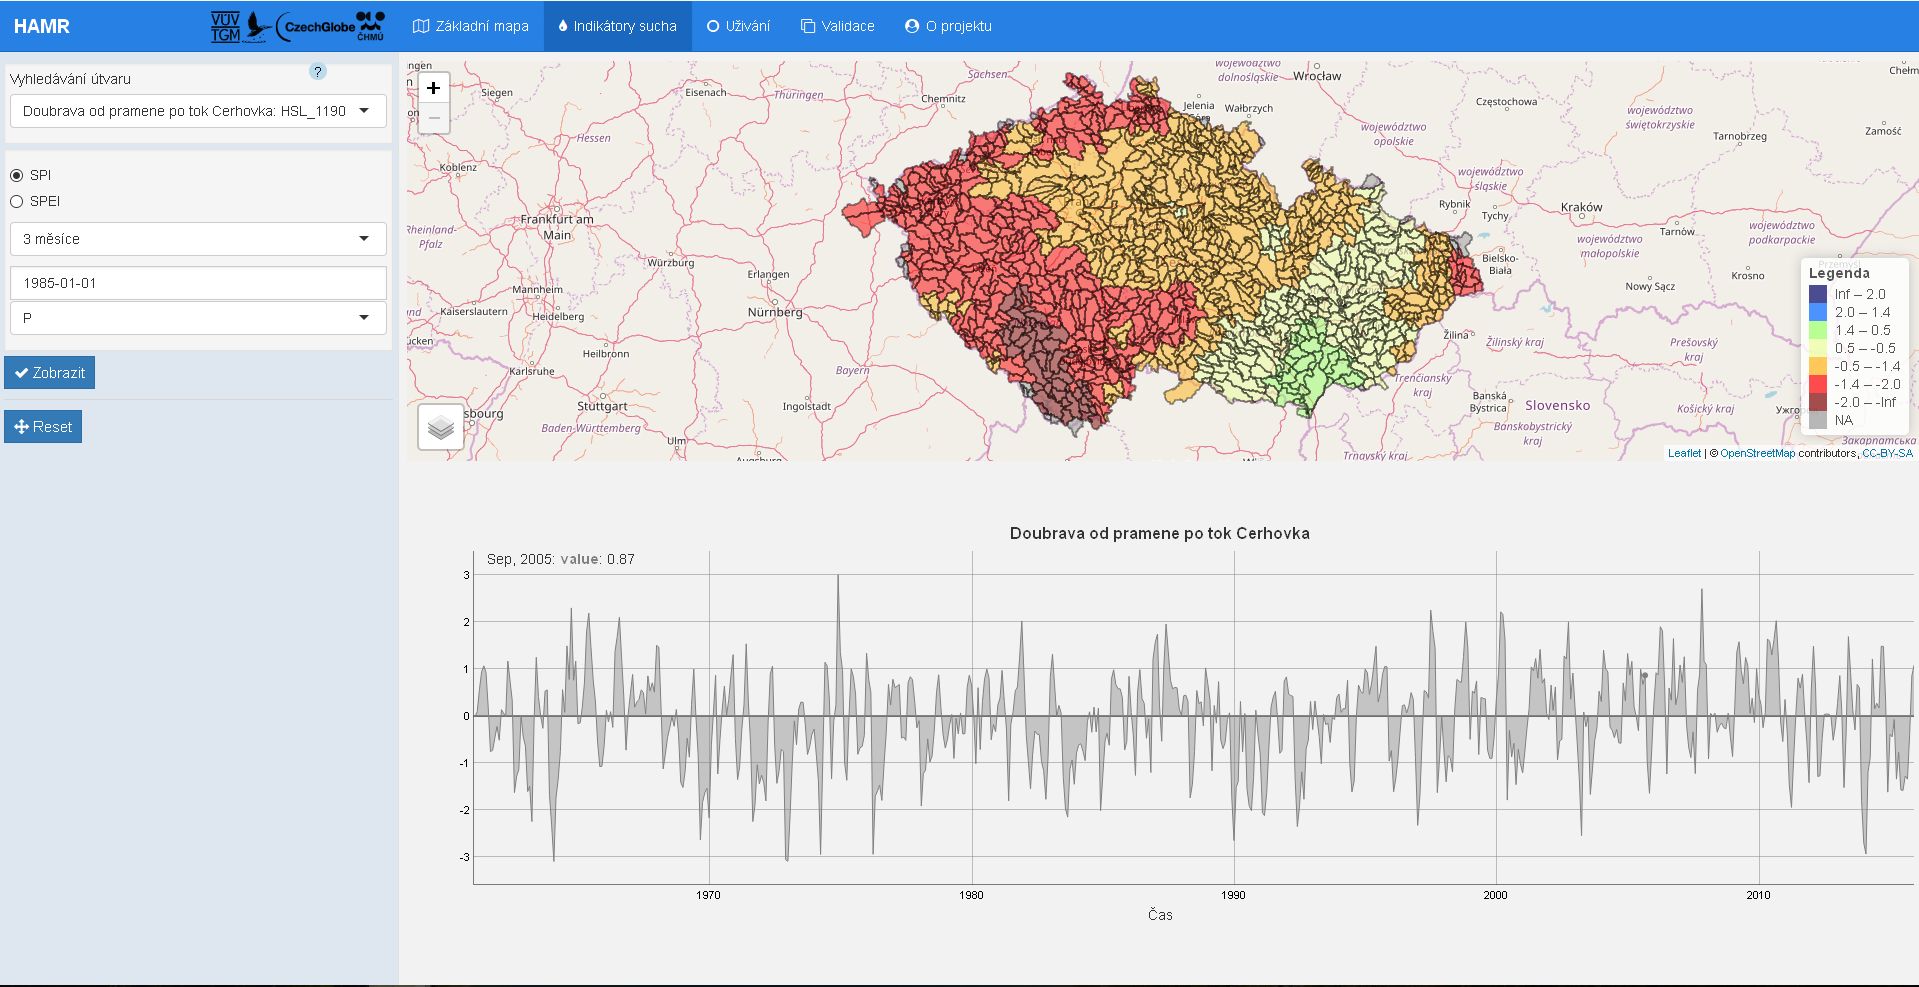
\includegraphics[width=\textwidth]{fig/P_indikatory}
      \caption{Záložka aplikace "Indikátory"}
      \label{fig:ch5.4}
\end{figure}

\vspace*{-0.3cm}

\qquad Záložka \enquote{Indikátory sucha} (obrázek \ref{fig:ch5.4}) se
skládá z bočního panelu, mapového panelu a grafického panelu. V bočním
panelu se obdobně jako v záložce \enquote{Základní mapa} nachází pole
\enquote{Vyhledávání útvaru} a \enquote{Vrstvy}. Dále v bočním panelu
lze zvolit indikátor a krok, do kterého budou data agregována. Dále lze
zvolit datum pro vykresleni mapy. Protože data mají měsíční časové
měřítko, volba konkrétního dne v kalendáře nehraje pro vykreslení žádnou
roli, ale v rámci \texttt{ui} volba data ve formátu
\enquote{\texttt{mm-YYYY}} zatím není možná. Momentálně v mapě jsou
zobrazeny indikátory SPI (\emph{Standardized Precipitation Index}) s
SPEI (\emph{Standardized Precipitation Evapotranspiration Index}), které
jsou počítány klouzavě s krokem 1, 3, 6, 9 a 12 měsíců. V~budoucích
verzích aplikace je plánováno přidání indikátorů PDSI (\emph{Palmer
Drought Severity Index}), SGI (\emph{Standardized Groundwater Index}),
SRI (\emph{Standardized Runoff Index}) a nedostatkových objemů ve
stejném kroku (Vlnas et al. 2014). Povodí se dělí do 7 kategorií podle
hodnoty příslušného indikátoru tak, aby se dostatečně projevila
variabilita:

\begin{table}[H]
\centering
\begin{tabular}{|c|c|}
\hline
$\infty$ až $2,0$   & extrémně vlhké    \\ \hline
$2,0$ až $1,4$      & silně vlhké       \\ \hline
$1,4$ až $0,5$      & mírně vlhké       \\ \hline
$0,5$ až $-0,5$     & bez výskytu sucha \\ \hline
$-0,5$ až $-1,4$    & slabé sucho       \\ \hline
$-1,4$ až $-2,0$    & silné sucho       \\ \hline
$-2,0$ až $-\infty$ & mimořádné sucho   \\ \hline
\end{tabular}
\caption{Rozdělení indikátorů sucha do kategorií.}
\label{tab9}
\end{table}

\vspace*{-0.3cm}

\qquad Mapové objekty jsou vykresleny pomocí \texttt{Leaflet}. V
grafický panelu se vykresluje časová řada indikátoru pro zvolené povodí
pomocí baličku \texttt{dygraphs}.

\subsubsection{6.3 Užívání}\label{uzivani}

\begin{figure}[H]
      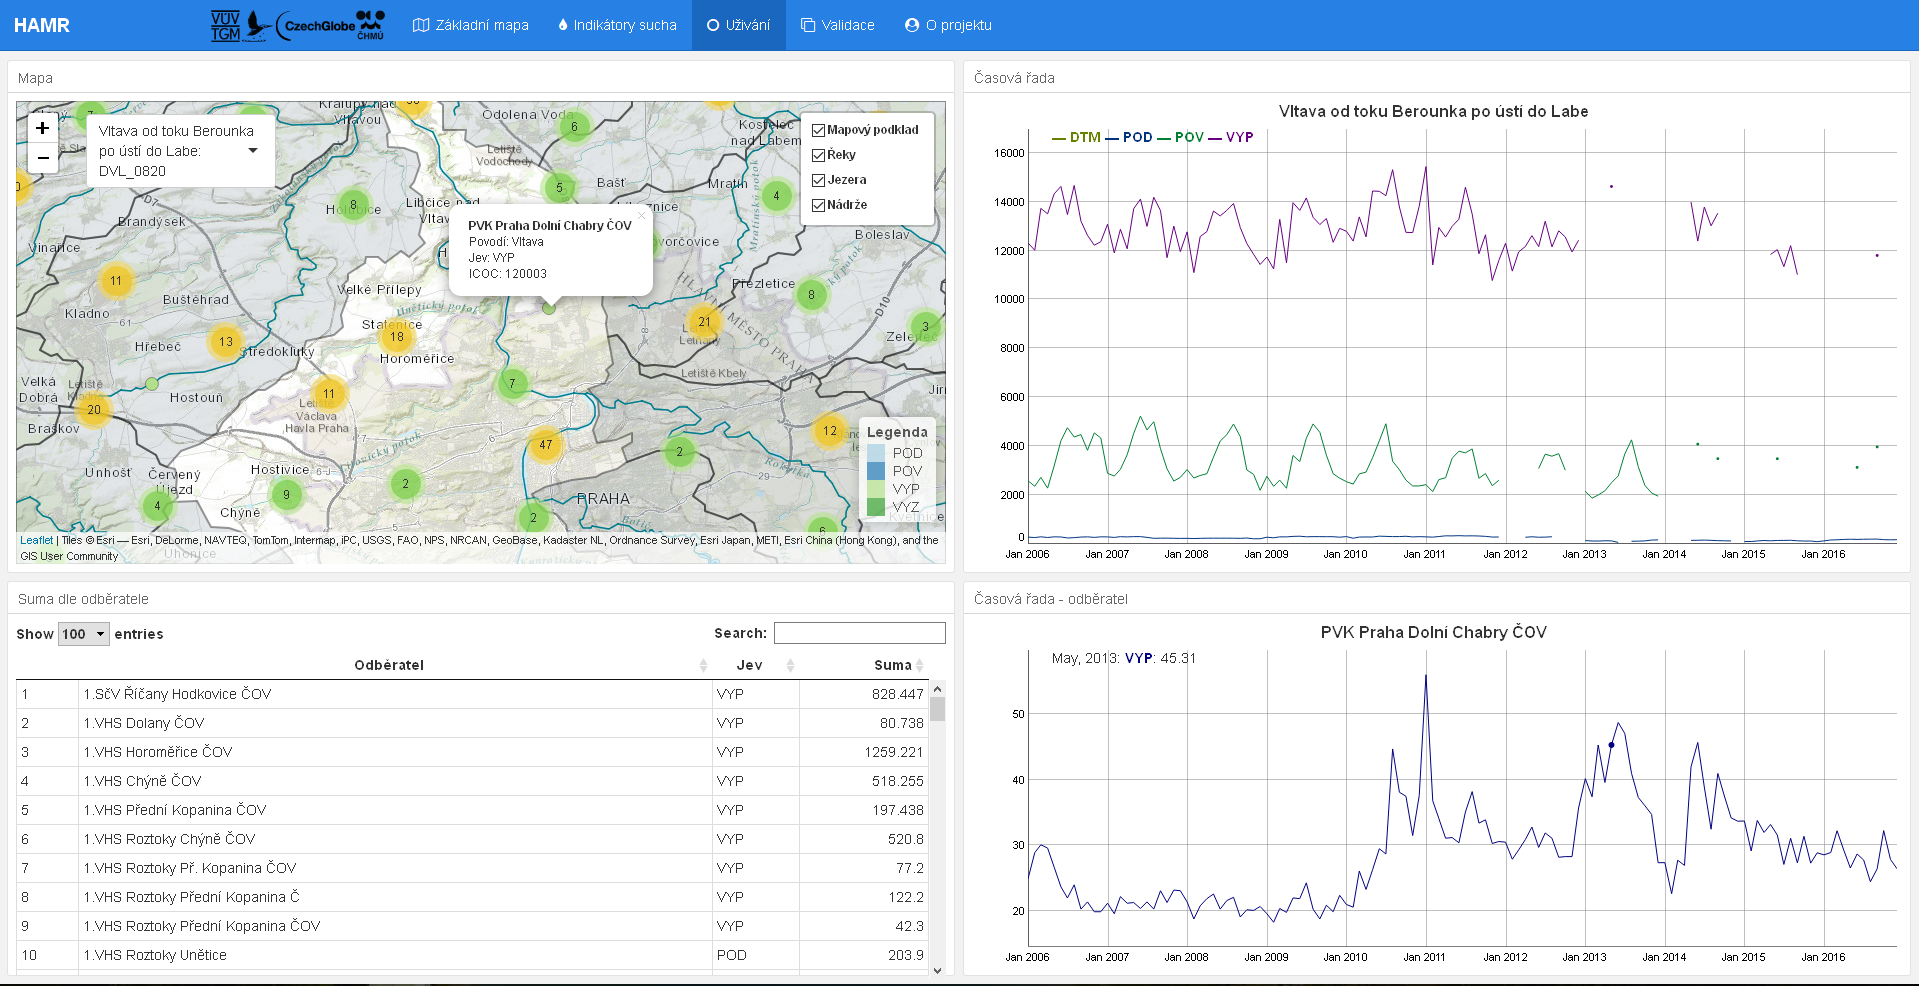
\includegraphics[width=\textwidth]{fig/P_uzivani}
      \caption{Záložka aplikace "Užívání"}
      \label{fig:ch5.5}
\end{figure}

\vspace*{-0.3cm}

\qquad Záložka \enquote{Užívání} (obrázek \ref{fig:ch5.5}) obsahuje
informace o užívání vody v ČR a~je rozdělena do pěti části: boční panel,
panel s mapovým výstupem, dva panely s~grafickými výstupy a jeden panel
s tabulkovým výstupem. Boční panel obsahuje pole \enquote{Vyhledávání
útvaru} a \enquote{Vrstvy}. Pole \enquote{Vrstvy} je rozšířeno o vrstvu
\enquote{Odběratele}, avšak postrádá administrativní členění České
republiky. Mapový panel spojuje místa odběru do shluků pomoci atributu
\texttt{clusterOptions\ =\ markerClusterOptions()} v~rámci funkce
\texttt{addCircleMarkers()} v \texttt{Leaflet}u. Po přiblížení lze na
bod kliknout. Po kliknutí se zobrazí popisek s informací o odběrateli a
vykreslí se časová řada odběrů. Kliknutím na povodí se obdrží informace
o všech odběratelích v tabulkovém panelu a~časová řada pro jednotlivé
jevy v grafickém panelu (odběry z podzemních vod \texttt{POD}, odběry z
povrchových vod \texttt{POV} či vypouštění \texttt{VYP}). Grafické
panely jsou vytvořený pomocí \texttt{dygraphs}. Tabulka je vytvořená
pomocí balíčku \texttt{DT} a je interaktivní.

\subsubsection{6.4 Validace}\label{validace}

\begin{figure}[H]
      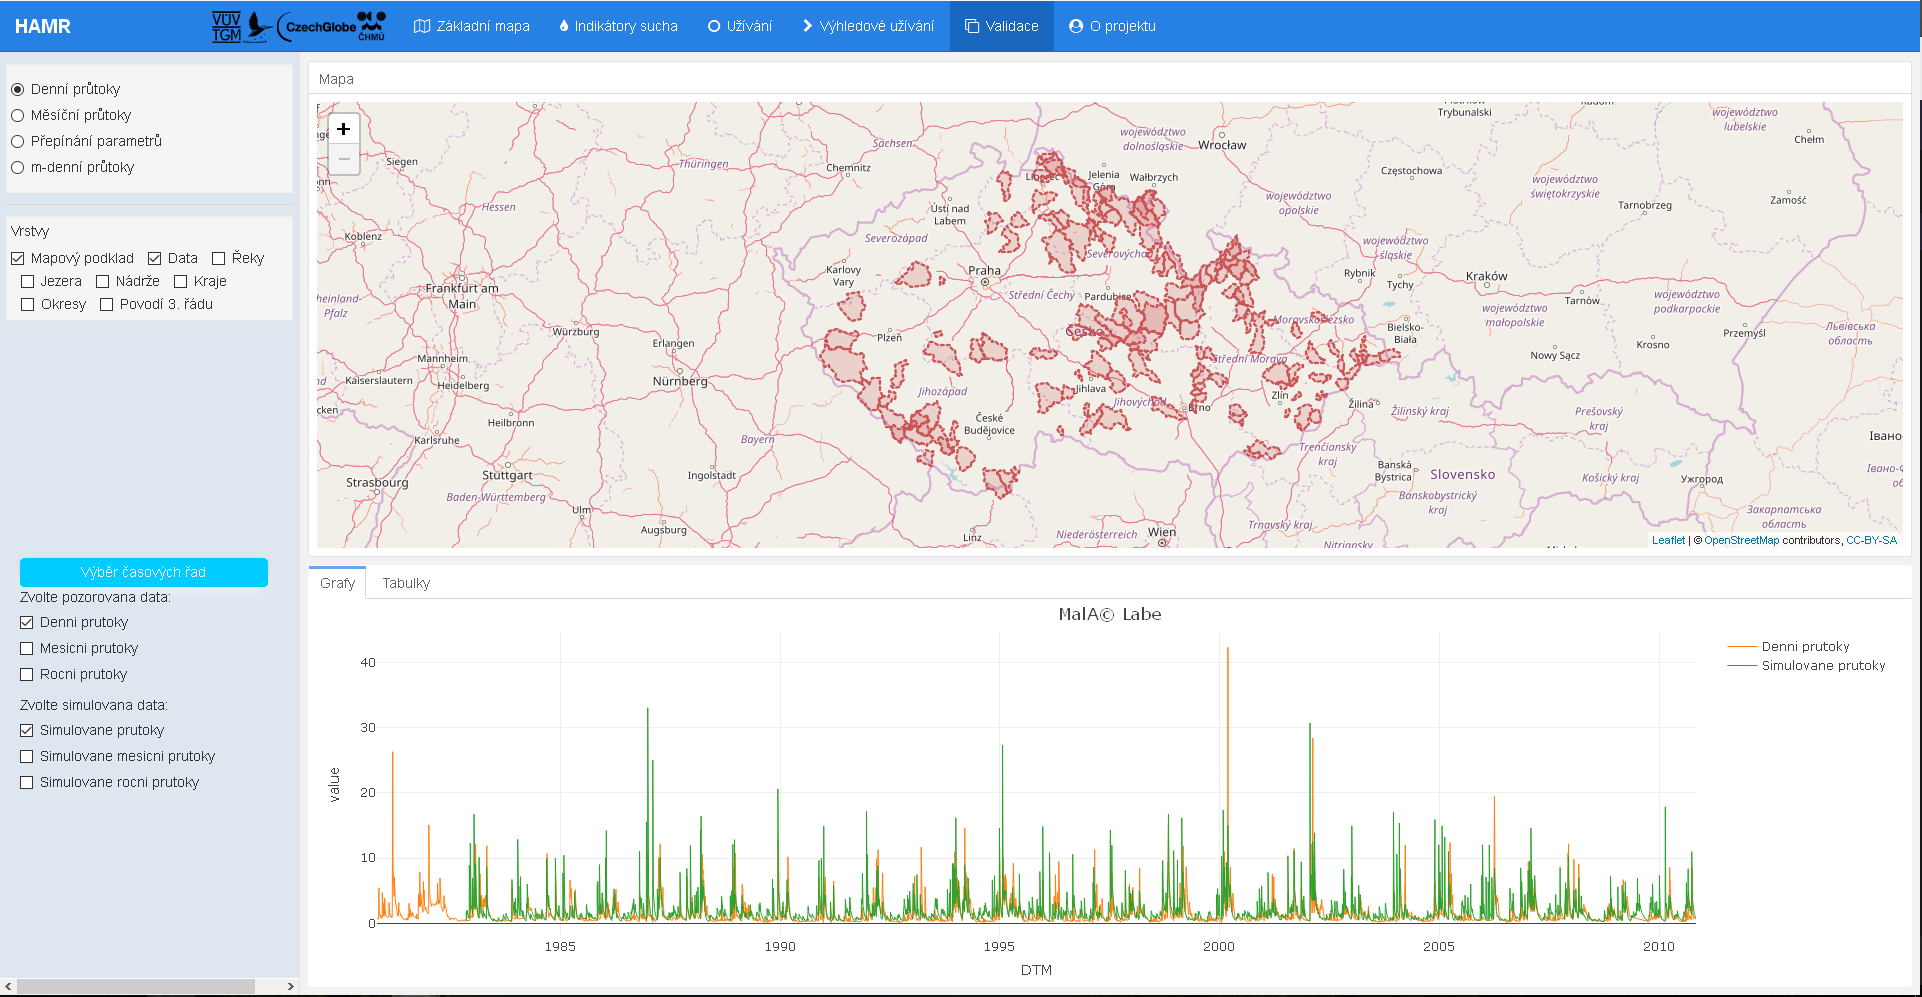
\includegraphics[width=\textwidth]{fig/P_validace}
      \caption{Záložka aplikace "Validace"}
      \label{fig:ch5.6}
\end{figure}

\vspace*{-0.3cm}

\qquad Záložka \enquote{Validace} (obrázek \ref{fig:ch5.6}) se dělí na
tří částí: boční panel, panel s mapovým výstupem a panel s grafickými
výstupem. Boční panel obsahuje standardní pole \enquote{Vrstvy} a
přepínač mezi následujícími možnostmi: denní průtoky, měsíční průtoky,
přepínání parametrů a m-denní průtoky.

\qquad Mapový výstup denních průtoků obsahuje polohu 153 měrných stanic
(viz kapitola \protect\hyperlink{data}{5.2}) a grafický panel po zvolení
konkrétní měrné stanice vytvoří časovou řadou pozorovaných a
simulovaných průtoků, které lze vykreslit v denním, měsíčním a~ročním
kroku pomocí menu \enquote{Výběr časových řad} (nachází se v oblastí
bočního panelu). Záložku grafického panelu lze přepnout z grafů na
tabulky, které nejsou interaktivní. Tabulka denních průtoků obsahuje
pouze základní přehled o datech (počet pozorování, střední hodnotu
atd.).

\qquad Mapový výstup měsíčních průtoků obsahuje pozice 542 vodoměrných
stanic. Body vodoměrných stanic jsou propojeny s informacemi o UPOVu, do
kterého spadají. Kliknutím na bod se objeví popisek stanice a vykreslí
se horní povodí, obdobně jako v záložce \enquote{Základní mapa}. Graf
obsahuje časové řady pozorovaných a~simulovaných průtoků a tabulka
obsahuje číselné vyhodnocení přesností simulovaných dat vůči pozorovaným
datům. Výpočet je uskutečněn pomocí funkce \texttt{gof()} z balíčku
\texttt{hydroGOR}\footnote{Dokumentace balíčku je dostupná na adrese
  \url{https://cran.r-project.org/web/packages/hydroGOF/hydroGOF.pdf}}.

\qquad Po zvolení \enquote{Přepínání parametrů} se v bočním panelu
objeví pole s nabídkou parametrů (\emph{Spa}, \emph{Alf}, \emph{Dgm},
\emph{Soc}, \emph{Mec}, \emph{Grd}). Momentálně \enquote{Přepínání
parametrů} obsahuje pouze panel s mapovým výstupem pro vizualizaci
plošného rozložení parametrů. UPOVy jsou zbarveny dle stávajících hodnot
parametru (\texttt{current}).

\qquad Po zvolení m-denních průtoků se objeví v bočním panelu nabídka
m-denních vod (\(Q30d\), \(Q60d\), \(Q90d\), \(Q120d\), \(Q150d\),
\(Q180d\), \(Q210d\), \(Q240d\), \(Q270d\), \(Q300d\), \(Q330d\),
\(Q355d\), \(Q364d\)). Také se objeví pole \enquote{Vyhledávání útvaru},
které propojuje mapový a~grafický panel. Útvary mapového výstupu se
zbarvují dle hodnoty proměnné, kterou zvolí uživatel. Grafickým výstupem
je \texttt{Plotly} objekt, který obsahuje seřazené hodnoty pozorovaných
a simulovaných m-denních průtoků pro zvolené povodí. Tabulkový výstup
obsahuje tytéž hodnoty.

\newpage

\section*{Výsledky}\label{vysledky}
\addcontentsline{toc}{section}{Výsledky}

\qquad Výsledkem práce je shrnutí klíčových poznatků týkajících se
vizualizace a průzkumové analýzy dat s jejich následnou praktickou
implementaci v R, a to v podobě webové interaktivní aplikace. Aplikace
slouží k analýze hydrologické bilance a předpovědi sucha v útvarech
povrchových vod České republiky. Hlavní funkcionalita aplikace spočívá v
její interaktivitě. Uživatel má možnost si prohlédnout data v různých
reprezentacích, a to například prostorové rozložení prvků hydrologické
bilance na území ČR, jejich časové řady, čáry překročení pro jednotlivé
útvary či plošné rozložení indikátorů sucha. Díky tomu si uživatel může
snadno vyhledat potřebné informace pro další analýzu a případný návrh
řešení problematiky sucha. Možnosti vlastního průzkumu dat, bez potřeby
znalosti programovacího jazyka, případně struktury souborů, v rámci
přehledné interaktivní aplikace je jedním z hlavních přínosu této práce.

\qquad Aplikace je dostupná v digitální podobě jak na přiloženým datovém
nosiči, tak i~na \href{https://shiny.fzp.czu.cz/KVHEM/HAMR/}{serveru
fakulty}\footnote{Aplikace na serveru fakulty:
  \url{https://shiny.fzp.czu.cz/KVHEM/HAMR/}} (viz kapitola
\protect\hyperlink{techres}{5.1}). Složky a soubory datového nosiče jsou
popsány v kapitole \protect\hyperlink{data}{5.2} a přehled jejich
struktury je znázorněn na obrázku \ref{fig:ch5.1}.

\newpage

\hypertarget{diskuse}{\section{Diskuse}\label{diskuse}}

\qquad Přestože aplikace je plně funkční, existuje prostor k jejímu
vylepšení a odladění nedostatků. Současná verze aplikace stále obsahuje
drobné chyby. Většina těchto chyb je způsobena chybami v používaných
balíčcích, jelikož jsou stále ve vývoji. Celkově je to nedostatek R,
které je distribuováno pod všeobecnou veřejnou licencí GNU GPL
(\emph{General Public License}) a neposkytuje absolutně žádné záruky.
Obdobně i většina balíčků neposkytuje záruky, ani uživatelskou podporu.
Z tohoto důvodu pro aplikaci byly zvoleny balíčky, které jsou stále
aktivně vyvíjeny, chyby jsou postupně odstraňovány a lze je vývojářům
nahlásit (například pomocí GitHub). Pro ostré nasazení systému (které se
výhledově ze strany Ministerstva životního prostředí předpokládá) bude
pravděpodobně nezbytné aplikaci přepsat do prostředí umožňujícího
rychlou vizualizaci komplexních geodat a dlouhých časových řad a~zároveň
zvládajícího vysokou návštěvnost uživatelů. Možností může být buď
placená verze Shiny serveru nebo platforma typu
\href{http://gisquick.org/}{GISQUICK}\footnote{GISQUICK je open source
  platformou pro publikování geoprostorových dat, viz
  \url{http://gisquick.org/}.}.

\qquad Další problém se kterým se R potýká je reprodukovatelnost
výsledků. S každou aktualizaci R a balíčků hrozí totiž ztráta plné
kompatibility. Pro finální verzí aplikace bude nutné se s tímto
problémem vypořádat. V současnosti existuje několik řešení, jako je
například balíček \texttt{checkpoint}, případně balíček
\texttt{packrat}.

\qquad První načtení aplikace trvá přibližně 40 vteřin\footnote{Měřeno
  na osobním počítači s konfigurací: i5-5200U, 8GB RAM, SSD.} a
přepínání mezi jednotlivými záložkami není okamžité. Lepšího výsledků by
mohlo být dosaženo pomocí načítání dat z databáze typu
\texttt{PostgreSQL}, \texttt{mongoDB} či jiného systému s rozhraním pro
R~(prostřednictvím balíčků \texttt{DBI} a \texttt{dbplyr}). Tento
přechod by avšak potřeboval odporných znalostí a měl by být důkladně
zvážen před bezprostřední implementací. Problém rychlostí aplikace by
mohlo také vyřešit její rozdělení do jednotlivých menších aplikací,
tento krok avšak vyvolává otázky o přehledností tohoto přístupu a
komfortu uživatele.

\newpage

\section*{Závěr}\label{zaver}
\addcontentsline{toc}{section}{Závěr}

\qquad V teoretické části je popsána historie a zásady vizualizace,
průzkumová analýza dat, základní a pokročilé vizualizační nástroje v R.
Na základě teoretické části je následně vytvořená interaktivní webová
aplikace pro analýzu hydrologické bilance a předpověď sucha v útvarech
povrchových vod ČR. Struktura a konkrétní řešení aplikace jsou podrobně
popsány v praktické části. Tato aplikace umožňuje uživateli průzkum dat
hydrologické bilance, časových řad prvků hydrologické bilance a jejich
čar překročení, plošné rozložení indikátorů sucha, míst užívání vod a
informaci o~odběratelích atd. Všechny tyto informace jsou v rámci
aplikace přehledně prezentovány a grafy jsou vytvořeny v souladu se
zásadami vizualizace dat.

\qquad Možné nedostatky jsou zmíněny v sekci
\protect\hyperlink{diskuse}{\enquote{Diskuse}} a zároveň jsou předložena
jejich možná řešení. Aplikace je v současné verzi plně funkční a
připravená k používání. Další vývoj bude podmíněn požadavky zadavatele a
uživatelů. Základní kostra aplikace umožňuje snadné rozšíření o další
záložky a implementace nových funkcí nepředstavuje žádný problém.

\newpage

\section{Literatura}\label{literatura}

\label{literatura}

\hypertarget{refs}{}
\hypertarget{ref-normalizing}{}
ABDI, Herve a LJ WILLIAMS, 2010. Normalizing data. Encyclopedia of
research design. \emph{Thousand Oaks, CA: Sage}.

\hypertarget{ref-trellisplot}{}
BECKER, Richard A, William S CLEVELAND, Ming-Jen SHYU, Stephen P KALUZNY
a OTHERS, 1996. A tour of Trellis graphics. \emph{Murray Hill, NJ: AT \&
T Bell Laboratories}.

\hypertarget{ref-brinton_1919}{}
BRINTON, Willard Cope, 1919. \emph{Graphic Methods for Presenting
Facts}. B.m.: The Engineering Magazine Company, New York.
ISBN~978-1155058870.

\hypertarget{ref-leverages_regression}{}
CARDINALI, C, 2014. Observation influence diagnostic of a data
assimilation system. \emph{Advanced Data Assimilation for Geosciences:
Lecture Notes of the Les Houches School of Physics: Special Issue}.
B.m.: Lecture Notes of the Les Houch.

\hypertarget{ref-chang2012}{}
CHANG, W., 2012. \emph{R Graphics Cookbook: Practical Recipes for
Visualizing Data}. B.m.: O'Reilly Media. ISBN~9781449363116.

\hypertarget{ref-spatial}{}
CHESHIRE, James a Robin LOVELACE, 2015. Spatial data visualisation with
R. \emph{Geocomputation: A Practical Primer}. B.m.: Sage.

\hypertarget{ref-cleveland1993}{}
CLEVELAND, William S., 1993. \emph{Visualizing Data}. B.m.: Hobart
Press. ISBN~978-0963488404.

\hypertarget{ref-cleveland1994}{}
CLEVELAND, William S., 1994. \emph{The Elements of Graphing Data}. B.m.:
Hobart Press. ISBN~0963488414.

\hypertarget{ref-cleveland_mcgill}{}
CLEVELAND, William S. a Robert MCGILL, 1984. Graphical Perception:
Theory, Experimentation, and Application to the Development of Graphical
Methods. \emph{Journal of the American Statistical Association}. B.m.:
Taylor \& Francis.

\hypertarget{ref-mbdist2}{}
DE MAESSCHALCK, Roy, Delphine JOUAN-RIMBAUD a Désiré L MASSART, 2000.
The mahalanobis distance. \emph{Chemometrics and intelligent laboratory
systems}. B.m.: Elsevier.

\hypertarget{ref-stackover}{}
DEVELOPER SURVEY RESULTS, 2017. \emph{Most Popular Languages by
Occupation} {[}online{]}. Dostupné
z:~\url{https://insights.stackoverflow.com/survey/2017\#technologies-and-occupations}

\hypertarget{ref-dplyr}{}
DPLYR, {[}vid. 17.4.2018{]}. \emph{A grammar of data manipulation.}
{[}online{]}. Dostupné z:~\url{https://github.com/tidyverse/dplyr}

\hypertarget{ref-bootstrap}{}
EFRON, B. a R.J. TIBSHIRANI, 1994. \emph{An Introduction to the
Bootstrap}. B.m.: Taylor \& Francis Ltd. ISBN~0-412-04231-2.

\hypertarget{ref-ferster}{}
FERSTER, Bill, 2012. \emph{Interactive Visualization: Insight through
Inquiry (MIT Press)}. B.m.: The MIT Press. ISBN~978-0262018159.

\hypertarget{ref-dataviz_history}{}
FRIENDLY, M., 2006. A Brief History of Data Visualization.
In:~\emph{Handbook of Computational Statistics: Data Visualization}.
B.m.: Springer-Verlag. ISBN~978-3-540-32825-4.

\hypertarget{ref-pp_wiki}{}
GIBBONS, Jean Dickinson a Subhabrata CHAKRABORTI, 2003.
\emph{Nonparametric Statistical Inference, Fourth Edition: Revised and
Expanded}. B.m.: CRC Press. ISBN~0-8247-4052-1.

\hypertarget{ref-vicerozm_stat}{}
HEBÁK, P, J HUSTOPECKÝ, E JAROŠOVÁ a I PECÁKOVÁ, 2007.
\emph{Vícerozměrné statistické metody (1)}. B.m.: Informatorium, Praha.
ISBN~80-7333-025-3.

\hypertarget{ref-spatial2}{}
HIJMANS, Robert, {[}vid. 13.4.2018{]}. \emph{Spatial Data Analysis and
Modeling with R} {[}online{]}. Dostupné z:~\url{http://rspatial.org/}

\hypertarget{ref-raster}{}
HIJMANS, Robert J., 2017. raster: Geographic Data Analysis and Modeling.
\emph{R package version 2.6-7} {[}online{]}. Dostupné
z:~\url{https://cran.r-project.org/web/packages/raster/raster.pdf}

\hypertarget{ref-kutner_transform}{}
KUTNER, Michael H, Christopher J. NACHTSHEIM, John NETER a William LI,
2004. \emph{Applied Linear Statistical Models}. B.m.: McGraw-Hill/Irwin.
ISBN~0-07-238688-6.

\hypertarget{ref-rasterVis}{}
LAMIGUEIRO, Oscar Perpinan, 2018. rasterVis: Visualization Methods for
Raster Data. \emph{R package version 0.44} {[}online{]}. Dostupné
z:~\url{https://cran.r-project.org/web/packages/rasterVis/rasterVis.pdf}

\hypertarget{ref-datarep2011}{}
MACIEJEWSKI, Ross, 2011. \emph{Data Representations, Transformations,
and Statistics for Visual Reasoning}. B.m.: Morgan \& Claypool
Publishers. ISBN~978-1-608-45625-3.

\hypertarget{ref-mbdist}{}
MAHALANOBIS, P. C., 1936. On the generalised distance in statistics.
\emph{Proceedings National Institute of Science}.

\hypertarget{ref-mcintosh2016}{}
MCINTOSH, Avery, 2016. The Jackknife Estimation Method. \emph{arXiv}.

\hypertarget{ref-minard1858}{}
MINARD, Charles Joseph, 1858. \emph{Carte figurative et approximative
représentant pour l'année 1858 les émigrants du globe, les pays dóu ils
partent et ceux oú ils arrivent} {[}online{]}. Dostupné
z:~\url{https://www.loc.gov/resource/g3201e.ct000242/}

\hypertarget{ref-murray}{}
MURRAY, Scott, 2013. \emph{Interactive Data Visualization for the Web}.
B.m.: O'Reilly Media. ISBN~978-1449339739.

\hypertarget{ref-murrell2003}{}
MURRELL, Paul, 2003. \emph{grid: The grid graphics package}.
červenec~2003.

\hypertarget{ref-murrell1998}{}
MURRELL, Paul R., 1998. \emph{Investigations in Graphical Statistics}.
B.m. PhD thesis. The University of Auckland.

\hypertarget{ref-novovic2006}{}
NOVOVIČOVÁ, Jana, 2006. \emph{Pravděpodobnost a matematická statistika}.
B.m.: Praha: Vydavatelství ČVUT, ISBN~80-01-01980-2.

\hypertarget{ref-normality_tests}{}
ÖZTUNA, Derya, Atilla Halil ELHAN a Ersöz TÜCCAR, 2006. Investigation of
four different normality tests in terms of type 1 error rate and power
under different distributions. \emph{Turkish Journal of Medical
Sciences}. B.m.: The Scientific; Technological Research Council of
Turkey.

\hypertarget{ref-palsky1996}{}
PALSKY, Gilles, 1996. \emph{Des chiffres et des cartes: naissance et
développement de la cartographie quantitative française au XIXe siecle}.
B.m.: Comité des travaux historiques et scientifiques-CTHS.

\hypertarget{ref-pecakova}{}
PECÁKOVÁ, Iva, 2014. Problém chybějících dat v dotazníkových šetřeních.
\emph{Politická ekonomie}. ISSN~2336-8225.

\hypertarget{ref-playfair1786}{}
PLAYFAIR, William, 1786. \emph{The Commercial and Political Atlas:
Representing, by Means of Stained Copper-plate Charts, the Exports,
Imports, and General Trade of England; the National Debt, And Other
Public Accounts; With Observations And Remarks: by William
Playfair,(author Of Regulations For The Interest Of Money.) To which are
Added, Charts of the Revenue and Debts of Ireland, Done In The Same
Manner, by James Corry, Esq. The Commercial Part is Taken from the
Custom-House Books, and the Public Accounts from the Journals of the
House of Commons, and Other Papers Belonging to that House Not Yet
Published}. B.m.: J. Debrett, Piccadilly; GG; J. Robinson, Pater-Noster
Row; J. Sewell, Cornhill; the engraver, SJ Neele, NO. 352, Strand; W.
Creech; C. Elliot, Edinburgh;; L. White, Dublin.

\hypertarget{ref-playfair1801}{}
PLAYFAIR, William, 1801. \emph{The Statistical Breviary: Shewing, on a
Principle Entirely New, the Resources of Every State and Kingdom in
Europe; Illustrated with Stained Copper-plate Charts the Physical Powers
of Each Distinct Nation with Ease and Perspicuity: to which is Added, a
Similar Exhibition of the Ruling Powers of Hindoostan}. B.m.: T.
Bensley, Bolt Court, Fleet Street.

\hypertarget{ref-plyr}{}
PLYR, {[}vid. 17.4.2018{]}. \emph{A R package for splitting, applying
and combining large problems into simpler problems.} {[}online{]}.
Dostupné z:~\url{https://github.com/hadley/plyr}

\hypertarget{ref-plot}{}
R-DOCUMENTATION, {[}vid. 11.5.2017{]}. \emph{Generic X-Y Plotting}
{[}online{]}. Dostupné
z:~\url{https://stat.ethz.ch/R-manual/R-devel/library/graphics/html/plot.html}

\hypertarget{ref-graphics}{}
R-DOCUMENTATION, {[}vid. 22.4.2017{]}. \emph{The R Graphics Package}
{[}online{]}. Dostupné
z:~\url{https://stat.ethz.ch/R-manual/R-devel/library/graphics/html/graphics-package.html}

\hypertarget{ref-datavis_rahlf}{}
RAHLF, Thomas, 2017. \emph{Data Visualisation with R: 100 Examples}.
B.m.: Springer. ISBN~978-3-319-49751-8.

\hypertarget{ref-rmarkdown}{}
RMARKDOWN, {[}vid. 16.4.2018{]}. \emph{Dynamic Documents for R}
{[}online{]}. Dostupné z:~\url{https://github.com/rstudio/rmarkdown}

\hypertarget{ref-dygraphs}{}
RSTUDIO, {[}vid. 11.4.2018{]}. \emph{dygraphs for R} {[}online{]}.
Dostupné z:~\url{http://rstudio.github.io/dygraphs/}

\hypertarget{ref-leaflet}{}
RSTUDIO, {[}vid. 11.4.2018{]}. \emph{Leaflet for R} {[}online{]}.
Dostupné z:~\url{http://rstudio.github.io/leaflet/}

\hypertarget{ref-shiny}{}
RSTUDIO, {[}vid. 14.4.2018{]}. \emph{Shiny from R Studio} {[}online{]}.
Dostupné z:~\url{https://shiny.rstudio.com/}

\hypertarget{ref-rstudio}{}
RSTUDIO, {[}vid. 16.4.2018{]}. \emph{RStudio - Open source and
enterprise-ready professional software for R} {[}online{]}. Dostupné
z:~\url{https://www.rstudio.com/}

\hypertarget{ref-SW_test}{}
SHAPIRO, S. S. a M. B. WILK, 1965. An analysis of variance test for
normality (complete samples)†. \emph{Biometrika}.

\hypertarget{ref-plotly}{}
SIEVERT, Carson, 2018. \emph{plotly for R} {[}online{]}. B.m.: bookdown.
Dostupné z:~\url{https://plotly-book.cpsievert.me/}

\hypertarget{ref-teetor2011}{}
TEETOR, P., 2011. \emph{R Cookbook: Proven Recipes for Data Analysis,
Statistics, and Graphics}. B.m.: O'Reilly Media. ISBN~9781449307264.

\hypertarget{ref-tidyr}{}
TIDYR, {[}vid. 17.4.2018{]}. \emph{Easily tidy data with spread and
gather functions.} {[}online{]}. Dostupné
z:~\url{https://github.com/tidyverse/tidyr}

\hypertarget{ref-tufte1983}{}
TUFTE, Edward R., 1983. \emph{The Visual Display of Quantitative
Information}. B.m.: Graphics Press. ISBN~978-0961392109.

\hypertarget{ref-tufte1990}{}
TUFTE, Edward R., 1990. \emph{Envisioning Information}. B.m.: Graphics
Pr. ISBN~978-0961392116.

\hypertarget{ref-jackknife_tukey}{}
TUKEY, John W., 1958. Bias and Confidence in Not Quite Large Samples.
\emph{Annals of Mathematical Statistics}.

\hypertarget{ref-tukey1962}{}
TUKEY, John W., 1962. The Future of Data Analysis. \emph{Annals of
Mathematical Statistics}. B.m.: The Institute of Mathematical
Statistics.

\hypertarget{ref-tukey1977}{}
TUKEY, John W., 1977. \emph{Exploratory Data Analysis}. B.m.:
Addison-Wesley. ISBN~0201076160.

\hypertarget{ref-htmlwidgets}{}
VAIDYANATHAN, Ramnath, Yihui XIE, JJ ALLAIRE, Joe CHENG a Kenton
RUSSELL, 2018. htmlwidgets: HTML Widgets for R. \emph{R package version
1.0} {[}online{]}. Dostupné
z:~\url{https://cran.r-project.org/web/packages/htmlwidgets/htmlwidgets.pdf}

\hypertarget{ref-bilan}{}
VIZINA, Adam, Stanislav HORÁČEK a Martin HANEL, 2015. Nové možnosti
modelu Bilan. \emph{Vodohospodářské technicko-ekonomické informace}.
B.m.: Výzkumný ústav vodohospodářský TG Masaryka, veřejná výzkumná
instituce.

\hypertarget{ref-sucho}{}
VLNAS, Radek, Adam BERAN, Martin HANEL, Anna HRABÁNKOVÁ, Tomáš HRDINKA,
Ladislav KAŠPÁREK, Marta MARTÍNKOVÁ, Martina PELÁKOVÁ, Pavel TREML, Adam
VIZINA, Petr BAŠTA, Lukáš JAČKA, Petr MÁCA, Jiří PAVLÁSEK a Pavel PECH,
2014. \emph{Metodika pro stanovení mezních hodnot indikátorů
hydrologického sucha}. Praha: Výzkumný ústav vodohospodářský TG
Masaryka, veřejná výzkumná instituce.

\hypertarget{ref-bilan_man}{}
VÚV TGM, 2015. \emph{Model hydrologické bilance Bilan}. B.m.: Výzkumný
ústav vodohospodářský TG Masaryka, veřejná výzkumná instituce.

\hypertarget{ref-layered-grammar}{}
WICKHAM, Hadley, 2010a. A layered grammar of graphics. \emph{Journal of
Computational and Graphical Statistics}.

\hypertarget{ref-wickham_ggplot}{}
WICKHAM, Hadley, 2010b. \emph{ggplot2: Elegant Graphics for Data
Analysis (Use R!)}. B.m.: Springer. ISBN~978-0387981406.

\hypertarget{ref-tidydata}{}
WICKHAM, Hadley, 2014. Tidy data. \emph{The Journal of Statistical
Software} {[}online{]}. Dostupné
z:~\url{http://www.jstatsoft.org/v59/i10/}

\hypertarget{ref-grolemund_wickham2017}{}
WICKHAM, Hadley a Garrett GROLEMUND, 2017. \emph{R for Data Science}.
B.m.: O'Reilly Media. ISBN~1491910399.

\hypertarget{ref-wilkinson2005}{}
WILKINSON, Leland, 2005. \emph{The Grammar of Graphics}. B.m.: Springer.
ISBN~9780387286952.

\hypertarget{ref-knitr}{}
XIE, Yihui, 2015. \emph{Dynamic Documents with R and Knitr}
{[}online{]}. B.m.: Boca Raton, Florida: Chapman; Hall/CRC. Dostupné
z:~\href{\%20http://yihui.name/knitr/}{ http://yihui.name/knitr/}

\hypertarget{ref-rmd:bookdown}{}
XIE, Yihui, 2018. \emph{Authoring Books and Technical Documents with R
Markdown}. B.m.: bookdown.

\hypertarget{ref-zumel_2014}{}
ZUMEL, Nina a John MOUNT, 2014. \emph{Practical Data Science with R}.
B.m.: Manning. ISBN~9781617291562.

\newpage

\section*{Poznamky}

\thispagestyle{empty}

(Minard 1858) (Palsky 1996)


\end{document}
